\documentclass[10pt,]{krantz}
\usepackage{lmodern}
\usepackage{amssymb,amsmath}
\usepackage{ifxetex,ifluatex}
\usepackage{fixltx2e} % provides \textsubscript
\ifnum 0\ifxetex 1\fi\ifluatex 1\fi=0 % if pdftex
  \usepackage[T1]{fontenc}
  \usepackage[utf8]{inputenc}
\else % if luatex or xelatex
  \ifxetex
    \usepackage{mathspec}
  \else
    \usepackage{fontspec}
  \fi
  \defaultfontfeatures{Ligatures=TeX,Scale=MatchLowercase}
    \setmonofont[Mapping=tex-ansi,Scale=0.7]{Source Code Pro}
\fi
% use upquote if available, for straight quotes in verbatim environments
\IfFileExists{upquote.sty}{\usepackage{upquote}}{}
% use microtype if available
\IfFileExists{microtype.sty}{%
\usepackage[]{microtype}
\UseMicrotypeSet[protrusion]{basicmath} % disable protrusion for tt fonts
}{}
\PassOptionsToPackage{hyphens}{url} % url is loaded by hyperref
\usepackage[unicode=true]{hyperref}
\PassOptionsToPackage{usenames,dvipsnames}{color} % color is loaded by hyperref
\hypersetup{
            pdftitle={R Programming - Lecture Notes},
            pdfauthor={Kyun-Seop Bae, Sungpil Han},
            colorlinks=true,
            linkcolor=Maroon,
            citecolor=Blue,
            urlcolor=Blue,
            breaklinks=true}
\urlstyle{same}  % don't use monospace font for urls
\usepackage{natbib}
\bibliographystyle{apalike}
\usepackage{color}
\usepackage{fancyvrb}
\newcommand{\VerbBar}{|}
\newcommand{\VERB}{\Verb[commandchars=\\\{\}]}
\DefineVerbatimEnvironment{Highlighting}{Verbatim}{commandchars=\\\{\}}
% Add ',fontsize=\small' for more characters per line
\usepackage{framed}
\definecolor{shadecolor}{RGB}{248,248,248}
\newenvironment{Shaded}{\begin{snugshade}}{\end{snugshade}}
\newcommand{\KeywordTok}[1]{\textcolor[rgb]{0.13,0.29,0.53}{\textbf{#1}}}
\newcommand{\DataTypeTok}[1]{\textcolor[rgb]{0.13,0.29,0.53}{#1}}
\newcommand{\DecValTok}[1]{\textcolor[rgb]{0.00,0.00,0.81}{#1}}
\newcommand{\BaseNTok}[1]{\textcolor[rgb]{0.00,0.00,0.81}{#1}}
\newcommand{\FloatTok}[1]{\textcolor[rgb]{0.00,0.00,0.81}{#1}}
\newcommand{\ConstantTok}[1]{\textcolor[rgb]{0.00,0.00,0.00}{#1}}
\newcommand{\CharTok}[1]{\textcolor[rgb]{0.31,0.60,0.02}{#1}}
\newcommand{\SpecialCharTok}[1]{\textcolor[rgb]{0.00,0.00,0.00}{#1}}
\newcommand{\StringTok}[1]{\textcolor[rgb]{0.31,0.60,0.02}{#1}}
\newcommand{\VerbatimStringTok}[1]{\textcolor[rgb]{0.31,0.60,0.02}{#1}}
\newcommand{\SpecialStringTok}[1]{\textcolor[rgb]{0.31,0.60,0.02}{#1}}
\newcommand{\ImportTok}[1]{#1}
\newcommand{\CommentTok}[1]{\textcolor[rgb]{0.56,0.35,0.01}{\textit{#1}}}
\newcommand{\DocumentationTok}[1]{\textcolor[rgb]{0.56,0.35,0.01}{\textbf{\textit{#1}}}}
\newcommand{\AnnotationTok}[1]{\textcolor[rgb]{0.56,0.35,0.01}{\textbf{\textit{#1}}}}
\newcommand{\CommentVarTok}[1]{\textcolor[rgb]{0.56,0.35,0.01}{\textbf{\textit{#1}}}}
\newcommand{\OtherTok}[1]{\textcolor[rgb]{0.56,0.35,0.01}{#1}}
\newcommand{\FunctionTok}[1]{\textcolor[rgb]{0.00,0.00,0.00}{#1}}
\newcommand{\VariableTok}[1]{\textcolor[rgb]{0.00,0.00,0.00}{#1}}
\newcommand{\ControlFlowTok}[1]{\textcolor[rgb]{0.13,0.29,0.53}{\textbf{#1}}}
\newcommand{\OperatorTok}[1]{\textcolor[rgb]{0.81,0.36,0.00}{\textbf{#1}}}
\newcommand{\BuiltInTok}[1]{#1}
\newcommand{\ExtensionTok}[1]{#1}
\newcommand{\PreprocessorTok}[1]{\textcolor[rgb]{0.56,0.35,0.01}{\textit{#1}}}
\newcommand{\AttributeTok}[1]{\textcolor[rgb]{0.77,0.63,0.00}{#1}}
\newcommand{\RegionMarkerTok}[1]{#1}
\newcommand{\InformationTok}[1]{\textcolor[rgb]{0.56,0.35,0.01}{\textbf{\textit{#1}}}}
\newcommand{\WarningTok}[1]{\textcolor[rgb]{0.56,0.35,0.01}{\textbf{\textit{#1}}}}
\newcommand{\AlertTok}[1]{\textcolor[rgb]{0.94,0.16,0.16}{#1}}
\newcommand{\ErrorTok}[1]{\textcolor[rgb]{0.64,0.00,0.00}{\textbf{#1}}}
\newcommand{\NormalTok}[1]{#1}
\usepackage{longtable,booktabs}
% Fix footnotes in tables (requires footnote package)
\IfFileExists{footnote.sty}{\usepackage{footnote}\makesavenoteenv{long table}}{}
\usepackage{graphicx,grffile}
\makeatletter
\def\maxwidth{\ifdim\Gin@nat@width>\linewidth\linewidth\else\Gin@nat@width\fi}
\def\maxheight{\ifdim\Gin@nat@height>\textheight\textheight\else\Gin@nat@height\fi}
\makeatother
% Scale images if necessary, so that they will not overflow the page
% margins by default, and it is still possible to overwrite the defaults
% using explicit options in \includegraphics[width, height, ...]{}
\setkeys{Gin}{width=\maxwidth,height=\maxheight,keepaspectratio}
\IfFileExists{parskip.sty}{%
\usepackage{parskip}
}{% else
\setlength{\parindent}{0pt}
\setlength{\parskip}{6pt plus 2pt minus 1pt}
}
\setlength{\emergencystretch}{3em}  % prevent overfull lines
\providecommand{\tightlist}{%
  \setlength{\itemsep}{0pt}\setlength{\parskip}{0pt}}
\setcounter{secnumdepth}{5}
% Redefines (sub)paragraphs to behave more like sections
\ifx\paragraph\undefined\else
\let\oldparagraph\paragraph
\renewcommand{\paragraph}[1]{\oldparagraph{#1}\mbox{}}
\fi
\ifx\subparagraph\undefined\else
\let\oldsubparagraph\subparagraph
\renewcommand{\subparagraph}[1]{\oldsubparagraph{#1}\mbox{}}
\fi

% set default figure placement to htbp
\makeatletter
\def\fps@figure{htbp}
\makeatother

\usepackage{booktabs}
\usepackage{longtable}
\usepackage[bf,singlelinecheck=off]{caption}

\usepackage{kotex}

\setmainfont[UprightFeatures={SmallCapsFont=AlegreyaSC-Regular}]{Alegreya}

\usepackage{framed,color}
\definecolor{shadecolor}{RGB}{248,248,248}

\renewcommand{\textfraction}{0.05}
\renewcommand{\topfraction}{0.8}
\renewcommand{\bottomfraction}{0.8}
\renewcommand{\floatpagefraction}{0.75}

\renewenvironment{quote}{\begin{VF}}{\end{VF}}
\let\oldhref\href
\renewcommand{\href}[2]{#2\footnote{\url{#1}}}

\ifxetex
  \usepackage{letltxmacro}
  \setlength{\XeTeXLinkMargin}{1pt}
  \LetLtxMacro\SavedIncludeGraphics\includegraphics
  \def\includegraphics#1#{% #1 catches optional stuff (star/opt. arg.)
    \IncludeGraphicsAux{#1}%
  }%
  \newcommand*{\IncludeGraphicsAux}[2]{%
    \XeTeXLinkBox{%
      \SavedIncludeGraphics#1{#2}%
    }%
  }%
\fi

\makeatletter
\newenvironment{kframe}{%
\medskip{}
\setlength{\fboxsep}{.8em}
 \def\at@end@of@kframe{}%
 \ifinner\ifhmode%
  \def\at@end@of@kframe{\end{minipage}}%
  \begin{minipage}{\columnwidth}%
 \fi\fi%
 \def\FrameCommand##1{\hskip\@totalleftmargin \hskip-\fboxsep
 \colorbox{shadecolor}{##1}\hskip-\fboxsep
     % There is no \\@totalrightmargin, so:
     \hskip-\linewidth \hskip-\@totalleftmargin \hskip\columnwidth}%
 \MakeFramed {\advance\hsize-\width
   \@totalleftmargin\z@ \linewidth\hsize
   \@setminipage}}%
 {\par\unskip\endMakeFramed%
 \at@end@of@kframe}
\makeatother

\renewenvironment{Shaded}{\begin{kframe}}{\end{kframe}}

\newenvironment{rmdblock}[1]
  {
  \begin{itemize}
  \renewcommand{\labelitemi}{
    \raisebox{-.7\height}[0pt][0pt]{
      {\setkeys{Gin}{width=3em,keepaspectratio}\includegraphics{images/#1}}
    }
  }
  \setlength{\fboxsep}{1em}
  \begin{kframe}
  \item
  }
  {
  \end{kframe}
  \end{itemize}
  }
\newenvironment{rmdnote}
  {\begin{rmdblock}{note}}
  {\end{rmdblock}}
\newenvironment{rmdcaution}
  {\begin{rmdblock}{caution}}
  {\end{rmdblock}}
\newenvironment{rmdimportant}
  {\begin{rmdblock}{important}}
  {\end{rmdblock}}
\newenvironment{rmdtip}
  {\begin{rmdblock}{tip}}
  {\end{rmdblock}}
\newenvironment{rmdwarning}
  {\begin{rmdblock}{warning}}
  {\end{rmdblock}}

\usepackage{makeidx}
\makeindex

\urlstyle{tt}

\usepackage{amsthm}
\makeatletter
\def\thm@space@setup{%
  \thm@preskip=8pt plus 2pt minus 4pt
  \thm@postskip=\thm@preskip
}
\makeatother

\frontmatter

\title{R Programming - Lecture Notes}
\author{Kyun-Seop Bae, Sungpil Han}
\date{2017-04-07}

\usepackage{amsthm}
\newtheorem{theorem}{Theorem}[chapter]
\newtheorem{lemma}{Lemma}[chapter]
\theoremstyle{definition}
\newtheorem{definition}{Definition}[chapter]
\newtheorem{corollary}{Corollary}[chapter]
\newtheorem{proposition}{Proposition}[chapter]
\theoremstyle{definition}
\newtheorem{example}{Example}[chapter]
\theoremstyle{remark}
\newtheorem*{remark}{Remark}
\begin{document}
\maketitle

%\cleardoublepage\newpage\thispagestyle{empty}\null
%\cleardoublepage\newpage\thispagestyle{empty}\null
%\cleardoublepage\newpage
\thispagestyle{empty}
\begin{center}
\includegraphics{images/cover.pdf}
\end{center}

\setlength{\abovedisplayskip}{-1pt}
\setlength{\abovedisplayshortskip}{-1pt}

{
\hypersetup{linkcolor=black}
\setcounter{tocdepth}{2}
\tableofcontents
}
\listoftables
\listoffigures
\chapter*{Preface}\label{preface}


안녕하십니까?

2017년 1학기 울산대학교 의학과 대학원 수업 \texttt{R\ Programming} 과목
담당교수 배균섭입니다.

R은 \url{http://cran.r-project.org} 에서 다운로드받아 설치할 수
있습니다. 역시 같은 사이트에서 Manual이 나와 있으니 참고하시기 바랍니다.
구글에서 `R Programming pdf'와 같은 키워드로 검색하시면 많은 자료를 보실
수 있습니다.

첨부한
\href{https://groups.google.com/a/acr.kr/group/r/attach/409db97bf453a/R.stx?part=0.1\&authuser=0}{R.stx}
파일은 AcroEdit이라는 editor에서 사용할 syntax highlighting용 구문
파일입니다. \url{http://www.acrosoft.pe.kr} 에서 다운로드 받아
설치하시기 바랍니다. AcroEdit대신 notepad++를 선호하시는 분은 그대로
사용하셔도 됩니다.

저는 RStudio, tinnR 등을 이용해서 강의하지 않습니다만, 필요하신 분은
쓰셔도 괜찮습니다. 향후 R package 작성을 위해서는 MiKTeX와 Rtools를
설치하십시오.

추가로 말씀드리자면, \url{http://www.coursera.org} 에 많은 R 강좌가
개설되어 있습니다. Specialization course로 들어가면 유로이지만,
(Specialization course는 여러 개의 과목이 합쳐져 있는 것입니다.) 개별
과목을 검색해서 들어가면, 무료로도 볼 수 있습니다. (대신 시험을 칠 수
없거나, certificate를 받을 수 없습니다.)

좋은 강좌가 많으니 많이 활용하시기 바립니다.

강의 장소에 불편함이 많은 것으로 생각되어, 다음과 같이 Skype 모임을
개설하였습니다. 사정상 원거리에서 오시기 불편한 분들은 활용하시기
바랍니다. 출석은 화면을 캡쳐하거나 휴대폰으로 찍은 뒤
\href{mailto:sec@acp.kr}{\nolinkurl{sec@acp.kr}},
\href{mailto:shan@acp.kr로}{\nolinkurl{shan@acp.kr로}} 보내주시면
출석으로 인정해 드립니다.

Skype 모임 참가 \url{https://meet.lync.com/uucp-acp/ksbae/SKGJ3BNQ}

2017년 3월, 배균섭 배상

The online version of this book is licensed under the
\href{http://creativecommons.org/licenses/by-nc-sa/4.0/}{Creative
Commons Attribution-NonCommercial-ShareAlike 4.0 International License}.

\begin{figure}
\centering
\includegraphics{images/by-nc-sa.png}
\caption{Creative Commons License}
\end{figure}

\section*{Teaching Assistant}\label{teaching-assistant}


안녕하십니까? 서울아산병원 임상약리학과 전공의 한성필입니다. 수업과
관련된 여러 제반 업무를 담당하고 있습니다. 언제든 의문사항 있으면
\href{mailto:r@acr.kr}{\nolinkurl{r@acr.kr}} 로 전체 메일 보내시거나
교수님 \href{mailto:k@acr.kr}{\nolinkurl{k@acr.kr}} 혹은 제 개인 메일
\href{mailto:shan@acp.kr로}{\nolinkurl{shan@acp.kr로}} 연락해 주십시오.

교수님께서 세우신 방침에 따라 수업시간에 출석을 부르지 않을 예정입니다.
수강하시는 화면(Skype)을 휴대폰으로 사진 찍으시거나 강의실의 스크린을
사진으로 촬영하셔서 \href{mailto:sec@acp.kr}{\nolinkurl{sec@acp.kr}} /
\href{mailto:shan@acp.kr}{\nolinkurl{shan@acp.kr}} 로 동시에 보내주시면
됩니다. 가급적 ``2017-03-31 한성필 출석'' 과 같은 식의 제목을 유지해
주시면 처리하는데 큰 도움이 될 것 같습니다.

\textbf{출석 체크를 위해 전체메일을 사용하지 말아주십시오!}

아울러 수업 중에 사용한 코드/스크립트를 사용하여 R의 패키지인
\texttt{bookdown}을 사용해 웹북을 제작 중에 있습니다. \citep{R-bookdown}
\index{bookdown} 여러분이 읽고 있는 이 책 자체가 R 코드의 일종인
\texttt{Rmarkdown}의 결과물이라고 보시면 됩니다.
\href{https://github.com/asancpt/Rprogramming}{Github 저장소}가 있으니
소스 코드를 보실 수 있습니다. 누구나 소스를 편집하여
\texttt{Pull\ Request}를 요청할 수 있으므로 혹시 Github를 사용하셔서
웹북의 질을 높이고자 하시는 수강생 선생님들께서는 도움을 주십시오.
\index{Github}

감사합니다.

2017년 3월, 한성필 올림

\section*{FAQ}\label{faq}


\subsection*{접속 관련}\label{-}


\begin{quote}
Q. 스카이프를 한번도 안써봐서 이참에 사용법을 배우고있는데, 수업시작시에
상대방을 어떻게 검색해서 들어가면 될지 알려주시면 감사하겠습니다.
\end{quote}

\begin{quote}
Q. 온라인 수강시 접속하는 스카이프 주소는 무엇인지요?
\end{quote}

\url{https://meet.lync.com/uucp-acp/ksbae/SKGJ3BNQ}

Chrome 등 웹브라우저에서 위 주소를 입력하면 직접 대화방으로 연결됩니다.
(검색할 필요 없습니다.) 처음 설치시에는 Add-on이 설치될 수 있습니다.
MacOS Sierra, Win7, Win10에서 Chrome, Internet Explorer 등을 사용하여
테스트해 보았고 모두 잘 동작하였습니다. 대부분의 경우 Skype For Business
계정이 없을 것으로 생각되는데 따로 로그인할 필요 없습니다.

수업 시작 30분 전부터 대화방을 개설해 놓도록 하겠습니다.

\url{https://groups.google.com/a/acr.kr/d/msg/r/nUkrE37W2kQ/waG-FkM_BgAJ}
교수님께서 처음 보낸 메일을 참고해 주십시오.

\begin{quote}
Q. 앞으로 수업은 지난 첫수업처럼 계속 온라인 수강이 가능한 것인가요?
\end{quote}

네, 계속 온라인으로 가능합니다.

\begin{quote}
Q. 저도 웹캠을 설치하여야 하여야 하나요?
\end{quote}

설치할 필요 없습니다. 오히려 수강자의 웹캠의 전원을 꺼두시길
권고드립니다.

\begin{quote}
Q. 수강전 온라인 강의 테스트 해볼 수 있나요?
\end{quote}

수업 시작 30분 전부터 대화방을 개설하여 놓도록 하겠습니다.

\subsection*{출석관련}


\begin{quote}
Q. 미국학회 참석으로 수업시간이 귀국행 비행기 기내에 있을거같아 출석이
안될것 같습니다. 방법이 있을지요?
\end{quote}

결석 사유서를 제출해 주시면 출석 처리 하겠습니다.
\href{http://www.medulsan.ac.kr/graduate/?mid=72\&curpage=files}{대학원
홈페이지 참고 바랍니다.} 이 링크로 들어가시면 가장 위에 있습니다.
(\texttt{결석사유서.hwp}) 참고로 수업 영상은 녹화하여 Youtube에 비공개
링크를 만들 예정이라서 추후에 관련 영상을 시청할 수 있을 것 같습니다.
결석사유서를 제출한다고 100\% 출석이 인정되는 것은 아닙니다. 이것이
기본적으로는 offline강의이기 때문에 강의시간에 강의실에 있든지, 또는
온라인으로 접속해 있어야 합니다. 출석사유서를 제출하거나, 추후 동영상
시청을 해서 그 증거(사진)을 제출하는 경우에 감점을 줄여드릴 수 있습니다.
예를 들어, 결석시에는 2점 감점인데, 결석사유서를 제출하면 1점만
감점한다는지, 동영상을 보면 0.5점만 감점한다는지 하는 것입니다. 결석
사유서 제출 시 출석 처리 원칙에 대한 설명을 드리오니, 참고하시길
바랍니다.

\subsection*{과제 관련}\label{-}


\begin{quote}
Q. 과제물이 있다고 들었는데 언제 assign하게 되는지요?
\end{quote}

과제물은 빨라야 5주차 이후에 나갑니다.

\subsection*{Coursera 관련}\label{coursera-}


\begin{quote}
Q. 첫 수업 때, certification 관련 말씀을 하셨는데, 정확히 coursera
사이트에서 어떤 것을 듣고, 제출을 해야하는지 궁금합니다. (비슷한 내용이
많아, 어떤것을 들어야하는지 헷갈립니다.) \index{Coursera}
\end{quote}

Coursera는 꼭 어느 것을 들어야 하는 것은 아니고, R programming과 관련된
것이라면 자유로이 골라서 들으면 됩니다. 대표적인 두 가지만 들자면 다음과
같습니다.

\begin{itemize}
\tightlist
\item
  \url{https://www.coursera.org/learn/r-programming}
\item
  \url{https://www.coursera.org/learn/r-programming-environment}
\end{itemize}

\begin{quote}
Q. Coursera 강의를 듣고 증명서를 내면 출석을 얼마나 커버할 수
있을런지요?
\end{quote}

Coursera는 출석 커버보다는 grade를 올려 주기 위한 것입니다. 출석은
Skype로 커버해야 합니다. 출석의 성적 반영비율은 25\%이지만, 규정상 4회
이상 결석이면 성적이 나갈 수 없습니다.

\section*{Syllabus}\label{syllabus}


\begin{figure}
\centering
\includegraphics{inst/Syllabus-0.png}
\caption{Syllabus page 1}
\end{figure}

\begin{figure}
\centering
\includegraphics{inst/Syllabus-1.png}
\caption{Syllabus page 2}
\end{figure}

\mainmatter

\chapter{R language}\label{r-language}

\begin{quote}
2017-03-15 배균섭 교수님 강의
\end{quote}

\href{https://cran.r-project.org/doc/manuals/r-release/R-lang.pdf}{R
Language Definition}의 초반 내용에 대해 설명하였습니다.

\chapter{Graphics}\label{graphics}

\begin{quote}
2017-03-22 임형석 교수님 강의
\end{quote}

R을 사용해 그림 그리는 방법에 대해 알아보겠습니다.

\section{Introduction}\label{introduction}

\begin{itemize}
\tightlist
\item
  상위수준 그림 함수는 그림을 생성한다.
\item
  하위수준 그림 함수는 기존의 그림에 그림을 추가한다.
\end{itemize}

\section{상위수준 그림 함수}\label{upper}

\subsection{상위수준 그림 함수의 주요 인자
(arguments)}\label{-----arguments}

\begin{itemize}
\tightlist
\item
  main : 제목
\item
  xlab/ylab : x축 및 y축 레이블
\item
  xlim/ylim : x축 및 y축 범위
\item
  col : 색깔
\item
  lty : 선 모양
\item
  pch : 점 모양
\item
  cex : 그림 성분의 크기
\item
  lwd : 선 굵기
\item
  type : 그림 타입
\end{itemize}

\begin{Shaded}
\begin{Highlighting}[]
\NormalTok{dta <-}\StringTok{ }\KeywordTok{read.csv}\NormalTok{(}\StringTok{"PK.csv"}\NormalTok{)}
\KeywordTok{head}\NormalTok{(dta)}
\end{Highlighting}
\end{Shaded}

\begin{verbatim}
##   ID TIME AMT    DV MDV
## 1  1 0.00   0  0.00   0
## 2  1 0.00   4  0.00   1
## 3  1 0.33   0  9.40   0
## 4  1 0.66   0 13.71   0
## 5  1 1.00   0 16.52   0
## 6  1 1.50   0 29.36   0
\end{verbatim}

\begin{Shaded}
\begin{Highlighting}[]
\KeywordTok{str}\NormalTok{(dta)}
\end{Highlighting}
\end{Shaded}

\begin{verbatim}
## 'data.frame':    456 obs. of  5 variables:
##  $ ID  : num  1 1 1 1 1 1 1 1 1 1 ...
##  $ TIME: num  0 0 0.33 0.66 1 1.5 2 3 4 6 ...
##  $ AMT : num  0 4 0 0 0 0 0 0 0 0 ...
##  $ DV  : num  0 0 9.4 13.7 16.5 ...
##  $ MDV : num  0 1 0 0 0 0 0 0 0 0 ...
\end{verbatim}

\subsection{scatter plot}\label{scatter-plot}

\begin{Shaded}
\begin{Highlighting}[]
\KeywordTok{plot}\NormalTok{(dta}\OperatorTok{$}\NormalTok{TIME[dta}\OperatorTok{$}\NormalTok{MDV}\OperatorTok{==}\DecValTok{0}\NormalTok{], dta}\OperatorTok{$}\NormalTok{DV[dta}\OperatorTok{$}\NormalTok{MDV}\OperatorTok{==}\DecValTok{0}\NormalTok{])}
\end{Highlighting}
\end{Shaded}

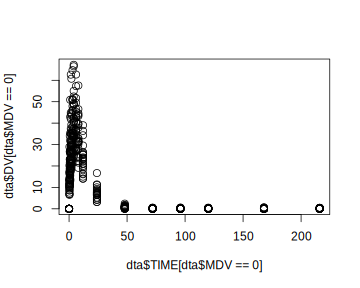
\includegraphics{Rprogramming_files/figure-latex/unnamed-chunk-3-1.pdf}

\begin{Shaded}
\begin{Highlighting}[]
\KeywordTok{plot}\NormalTok{(dta}\OperatorTok{$}\NormalTok{TIME[dta}\OperatorTok{$}\NormalTok{MDV}\OperatorTok{==}\DecValTok{0}\NormalTok{], dta}\OperatorTok{$}\NormalTok{DV[dta}\OperatorTok{$}\NormalTok{MDV}\OperatorTok{==}\DecValTok{0}\NormalTok{], }\DataTypeTok{log=}\StringTok{"y"}\NormalTok{)}
\end{Highlighting}
\end{Shaded}

\begin{verbatim}
## Warning in xy.coords(x, y, xlabel, ylabel, log): 86 y
## values <= 0 omitted from logarithmic plot
\end{verbatim}

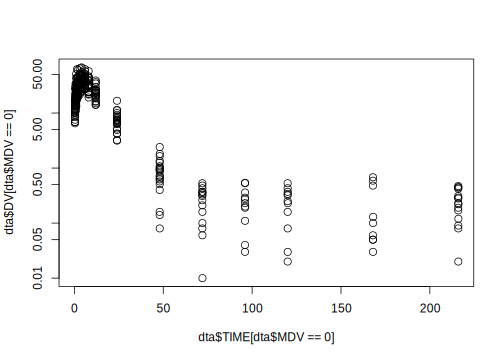
\includegraphics{Rprogramming_files/figure-latex/unnamed-chunk-3-2.pdf}

\begin{Shaded}
\begin{Highlighting}[]
\KeywordTok{plot}\NormalTok{(dta}\OperatorTok{$}\NormalTok{TIME[dta}\OperatorTok{$}\NormalTok{MDV}\OperatorTok{==}\DecValTok{0}\NormalTok{], }\KeywordTok{log}\NormalTok{(dta}\OperatorTok{$}\NormalTok{DV[dta}\OperatorTok{$}\NormalTok{MDV}\OperatorTok{==}\DecValTok{0}\NormalTok{]))}
\end{Highlighting}
\end{Shaded}

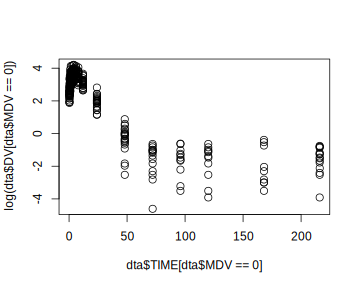
\includegraphics{Rprogramming_files/figure-latex/unnamed-chunk-3-3.pdf}

\begin{Shaded}
\begin{Highlighting}[]
\KeywordTok{plot}\NormalTok{(dta}\OperatorTok{$}\NormalTok{TIME[dta}\OperatorTok{$}\NormalTok{MDV}\OperatorTok{==}\DecValTok{0}\NormalTok{], dta}\OperatorTok{$}\NormalTok{DV[dta}\OperatorTok{$}\NormalTok{MDV}\OperatorTok{==}\DecValTok{0}\NormalTok{]}
\NormalTok{     , }\DataTypeTok{xlab=}\StringTok{"Time (hr)"}\NormalTok{, }\DataTypeTok{ylab=}\StringTok{"Concentration (ng/mL)"} 
\NormalTok{     , }\DataTypeTok{type=}\StringTok{"o"}\NormalTok{, }\DataTypeTok{pch=}\DecValTok{2}\NormalTok{, }\DataTypeTok{col=}\DecValTok{1}\NormalTok{, }\DataTypeTok{main=}\StringTok{"PK time-course of Drug X"}
\NormalTok{     , }\DataTypeTok{xlim =}\KeywordTok{c}\NormalTok{(}\OperatorTok{-}\DecValTok{2}\NormalTok{,}\DecValTok{218}\NormalTok{), }\DataTypeTok{ylim=}\KeywordTok{c}\NormalTok{(}\DecValTok{0}\NormalTok{,}\DecValTok{80}\NormalTok{))}
\end{Highlighting}
\end{Shaded}

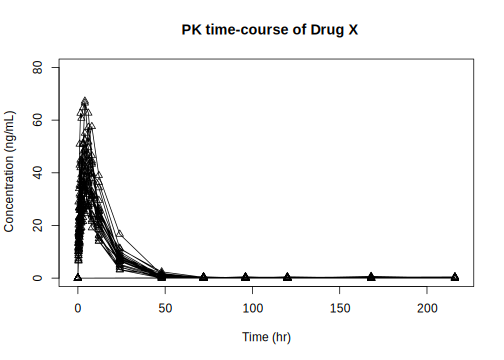
\includegraphics{Rprogramming_files/figure-latex/unnamed-chunk-3-4.pdf}

\begin{Shaded}
\begin{Highlighting}[]
\KeywordTok{plot}\NormalTok{(dta}\OperatorTok{$}\NormalTok{TIME[dta}\OperatorTok{$}\NormalTok{MDV}\OperatorTok{==}\DecValTok{0}\NormalTok{], dta}\OperatorTok{$}\NormalTok{DV[dta}\OperatorTok{$}\NormalTok{MDV}\OperatorTok{==}\DecValTok{0}\NormalTok{], }\DataTypeTok{axes=}\NormalTok{F,}
\NormalTok{     , }\DataTypeTok{xlab=}\StringTok{"Time (hr)"}\NormalTok{, }\DataTypeTok{ylab=}\StringTok{"Concentration (ng/mL)"} 
\NormalTok{     , }\DataTypeTok{type=}\StringTok{"o"}\NormalTok{, }\DataTypeTok{pch=}\DecValTok{2}\NormalTok{, }\DataTypeTok{col=}\DecValTok{1}\NormalTok{, }\DataTypeTok{main=}\StringTok{"PK time-course of Drug X"}
\NormalTok{     , }\DataTypeTok{xlim =}\KeywordTok{c}\NormalTok{(}\OperatorTok{-}\DecValTok{2}\NormalTok{,}\DecValTok{218}\NormalTok{), }\DataTypeTok{ylim=}\KeywordTok{c}\NormalTok{(}\DecValTok{0}\NormalTok{,}\DecValTok{80}\NormalTok{))}
\KeywordTok{axis}\NormalTok{(}\DecValTok{1}\NormalTok{, }\DataTypeTok{at=}\KeywordTok{seq}\NormalTok{(}\DecValTok{0}\NormalTok{, }\DecValTok{218}\NormalTok{, }\DecValTok{24}\NormalTok{))}
\KeywordTok{axis}\NormalTok{(}\DecValTok{2}\NormalTok{)}
\KeywordTok{box}\NormalTok{()}
\end{Highlighting}
\end{Shaded}

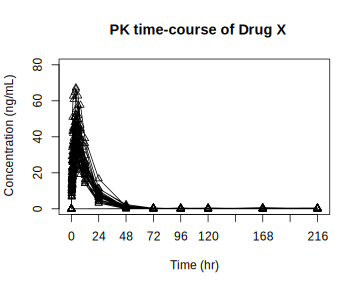
\includegraphics{Rprogramming_files/figure-latex/unnamed-chunk-3-5.pdf}

\subsection{Histogram}\label{histogram}

\begin{Shaded}
\begin{Highlighting}[]
\NormalTok{d.demog <-}\StringTok{ }\KeywordTok{read.csv}\NormalTok{(}\StringTok{"DEMOG.csv"}\NormalTok{)}

\KeywordTok{hist}\NormalTok{(d.demog}\OperatorTok{$}\NormalTok{HT)}
\end{Highlighting}
\end{Shaded}

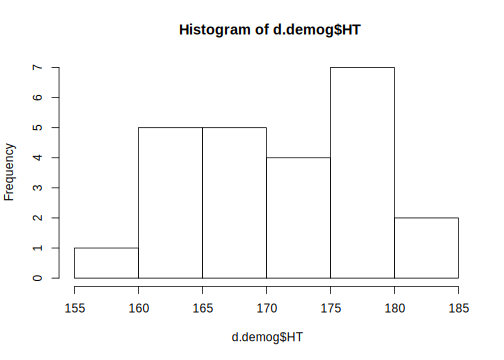
\includegraphics{Rprogramming_files/figure-latex/unnamed-chunk-4-1.pdf}

\begin{Shaded}
\begin{Highlighting}[]
\KeywordTok{hist}\NormalTok{(d.demog}\OperatorTok{$}\NormalTok{HT, }\DataTypeTok{breaks=}\DecValTok{10}\NormalTok{)}
\KeywordTok{hist}\NormalTok{(d.demog}\OperatorTok{$}\NormalTok{HT, }\DataTypeTok{nclass=}\DecValTok{10}\NormalTok{)}
\end{Highlighting}
\end{Shaded}

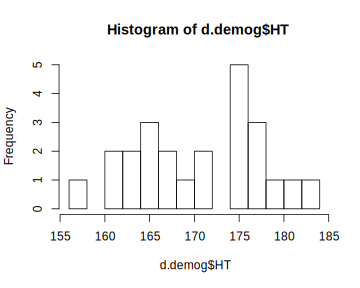
\includegraphics{Rprogramming_files/figure-latex/unnamed-chunk-4-2.pdf}

\subsubsection{with density line}\label{with-density-line}

\begin{Shaded}
\begin{Highlighting}[]
\KeywordTok{hist}\NormalTok{ (d.demog}\OperatorTok{$}\NormalTok{HT, }\DataTypeTok{probability=}\OtherTok{TRUE}\NormalTok{, }\DataTypeTok{breaks=}\DecValTok{10}\NormalTok{)}
\KeywordTok{lines}\NormalTok{(}\KeywordTok{density}\NormalTok{(d.demog}\OperatorTok{$}\NormalTok{HT))}
\end{Highlighting}
\end{Shaded}

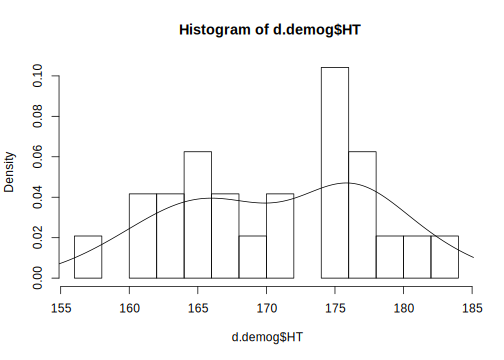
\includegraphics{Rprogramming_files/figure-latex/unnamed-chunk-5-1.pdf}

\begin{Shaded}
\begin{Highlighting}[]
\KeywordTok{hist}\NormalTok{ (d.demog}\OperatorTok{$}\NormalTok{HT, }\DataTypeTok{probability=}\OtherTok{TRUE}\NormalTok{, }\DataTypeTok{breaks=}\DecValTok{9}\NormalTok{, }\DataTypeTok{xaxt=}\StringTok{"n"}
\NormalTok{      , }\DataTypeTok{main=}\StringTok{"Histogram for Height"}\NormalTok{, }\DataTypeTok{xlab=}\StringTok{"Height (cm)"}\NormalTok{, }\DataTypeTok{ylab=}\StringTok{"Probability (%)"}\NormalTok{)}
\KeywordTok{axis}\NormalTok{(}\DecValTok{1}\NormalTok{, }\DataTypeTok{at=}\KeywordTok{seq}\NormalTok{(}\KeywordTok{min}\NormalTok{(d.demog}\OperatorTok{$}\NormalTok{HT), }\KeywordTok{max}\NormalTok{(d.demog}\OperatorTok{$}\NormalTok{HT), }\DecValTok{3}\NormalTok{))}
\KeywordTok{lines}\NormalTok{(}\KeywordTok{density}\NormalTok{(d.demog}\OperatorTok{$}\NormalTok{HT))}
\end{Highlighting}
\end{Shaded}

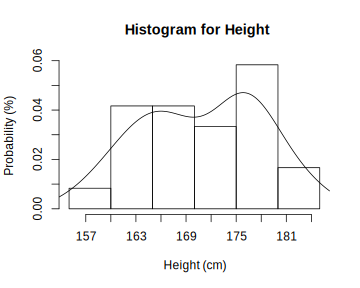
\includegraphics{Rprogramming_files/figure-latex/unnamed-chunk-5-2.pdf}

\begin{Shaded}
\begin{Highlighting}[]
\KeywordTok{hist}\NormalTok{ (d.demog}\OperatorTok{$}\NormalTok{HT, }\DataTypeTok{probability=}\OtherTok{TRUE}\NormalTok{, }\DataTypeTok{breaks=}\DecValTok{9}\NormalTok{, }\DataTypeTok{xaxt=}\StringTok{"n"}
\NormalTok{      , }\DataTypeTok{main=}\StringTok{"Histogram for Height"}\NormalTok{, }\DataTypeTok{xlab=}\StringTok{"Height (cm)"}\NormalTok{, }\DataTypeTok{ylab=}\StringTok{"Probability (%)"}
\NormalTok{      , }\DataTypeTok{col =} \StringTok{"lightblue"}\NormalTok{, }\DataTypeTok{border =} \StringTok{"pink"}\NormalTok{)}
\KeywordTok{axis}\NormalTok{(}\DecValTok{1}\NormalTok{, }\DataTypeTok{at=}\KeywordTok{seq}\NormalTok{(}\KeywordTok{min}\NormalTok{(d.demog}\OperatorTok{$}\NormalTok{HT), }\KeywordTok{max}\NormalTok{(d.demog}\OperatorTok{$}\NormalTok{HT), }\DecValTok{3}\NormalTok{))}
\KeywordTok{lines}\NormalTok{(}\KeywordTok{density}\NormalTok{(d.demog}\OperatorTok{$}\NormalTok{HT))}
\end{Highlighting}
\end{Shaded}

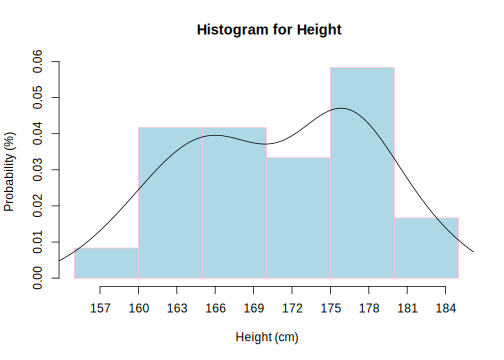
\includegraphics{Rprogramming_files/figure-latex/unnamed-chunk-5-3.pdf}

\subsection{Box-Whisker Plot}\label{box-whisker-plot}

\begin{Shaded}
\begin{Highlighting}[]
\KeywordTok{boxplot}\NormalTok{(d.demog}\OperatorTok{$}\NormalTok{WT)}
\end{Highlighting}
\end{Shaded}

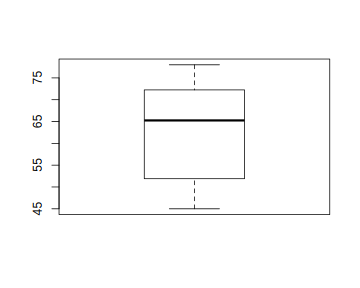
\includegraphics{Rprogramming_files/figure-latex/unnamed-chunk-6-1.pdf}

\begin{Shaded}
\begin{Highlighting}[]
\KeywordTok{boxplot}\NormalTok{(d.demog}\OperatorTok{$}\NormalTok{WT }\OperatorTok{~}\StringTok{ }\NormalTok{d.demog}\OperatorTok{$}\NormalTok{SEX)}

\KeywordTok{boxplot}\NormalTok{(}\KeywordTok{split}\NormalTok{(d.demog}\OperatorTok{$}\NormalTok{WT, d.demog}\OperatorTok{$}\NormalTok{SEX))}
\end{Highlighting}
\end{Shaded}

\includegraphics{Rprogramming_files/figure-latex/unnamed-chunk-6-2.pdf}

\begin{Shaded}
\begin{Highlighting}[]
\KeywordTok{boxplot}\NormalTok{(WT }\OperatorTok{~}\StringTok{ }\NormalTok{SEX, }\DataTypeTok{data=}\NormalTok{d.demog)}

\KeywordTok{boxplot}\NormalTok{(d.demog}\OperatorTok{$}\NormalTok{WT }\OperatorTok{~}\StringTok{ }\NormalTok{d.demog}\OperatorTok{$}\NormalTok{SEX}
\NormalTok{        , }\DataTypeTok{names=}\KeywordTok{c}\NormalTok{(}\StringTok{"Male"}\NormalTok{,}\StringTok{"Female"}\NormalTok{), }\DataTypeTok{ylab=}\StringTok{"AGE, year"}\NormalTok{, }\DataTypeTok{ylim=}\KeywordTok{c}\NormalTok{(}\KeywordTok{min}\NormalTok{(d.demog}\OperatorTok{$}\NormalTok{WT)}\OperatorTok{-}\DecValTok{2}\NormalTok{, }\KeywordTok{max}\NormalTok{(d.demog}\OperatorTok{$}\NormalTok{WT)}\OperatorTok{+}\DecValTok{2}\NormalTok{)}
\NormalTok{        , }\DataTypeTok{col=}\StringTok{"pink"}\NormalTok{)}
\end{Highlighting}
\end{Shaded}

\includegraphics{Rprogramming_files/figure-latex/unnamed-chunk-6-3.pdf}

\begin{Shaded}
\begin{Highlighting}[]
\KeywordTok{boxplot}\NormalTok{(d.demog}\OperatorTok{$}\NormalTok{WT }\OperatorTok{~}\StringTok{ }\NormalTok{d.demog}\OperatorTok{$}\NormalTok{SEX}
\NormalTok{        , }\DataTypeTok{names=}\KeywordTok{c}\NormalTok{(}\StringTok{"Male"}\NormalTok{,}\StringTok{"Female"}\NormalTok{), }\DataTypeTok{ylab=}\StringTok{"AGE, year"}\NormalTok{, }\DataTypeTok{ylim=}\KeywordTok{c}\NormalTok{(}\KeywordTok{min}\NormalTok{(d.demog}\OperatorTok{$}\NormalTok{WT)}\OperatorTok{-}\DecValTok{2}\NormalTok{, }\KeywordTok{max}\NormalTok{(d.demog}\OperatorTok{$}\NormalTok{WT)}\OperatorTok{+}\DecValTok{2}\NormalTok{)}
\NormalTok{        , }\DataTypeTok{col=}\KeywordTok{c}\NormalTok{(}\StringTok{"lightblue"}\NormalTok{, }\StringTok{"salmon"}\NormalTok{), }\DataTypeTok{width=}\KeywordTok{c}\NormalTok{(}\FloatTok{0.6}\NormalTok{, }\DecValTok{1}\NormalTok{))}
\end{Highlighting}
\end{Shaded}

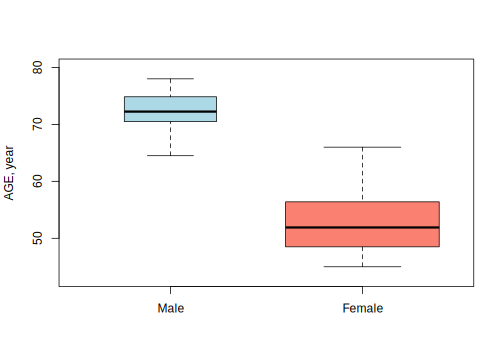
\includegraphics{Rprogramming_files/figure-latex/unnamed-chunk-6-4.pdf}

-varwidth: if varwidth is TRUE, the boxes are drawn with widths
proportional to the square-roots of the number of observations in the
groups.

\begin{Shaded}
\begin{Highlighting}[]
\KeywordTok{boxplot}\NormalTok{(d.demog}\OperatorTok{$}\NormalTok{WT }\OperatorTok{~}\StringTok{ }\NormalTok{d.demog}\OperatorTok{$}\NormalTok{SEX}
\NormalTok{        , }\DataTypeTok{names=}\KeywordTok{c}\NormalTok{(}\StringTok{"Male"}\NormalTok{,}\StringTok{"Female"}\NormalTok{), }\DataTypeTok{ylab=}\StringTok{"AGE, year"}\NormalTok{, }\DataTypeTok{ylim=}\KeywordTok{c}\NormalTok{(}\KeywordTok{min}\NormalTok{(d.demog}\OperatorTok{$}\NormalTok{WT)}\OperatorTok{-}\DecValTok{2}\NormalTok{, }\KeywordTok{max}\NormalTok{(d.demog}\OperatorTok{$}\NormalTok{WT)}\OperatorTok{+}\DecValTok{2}\NormalTok{)}
\NormalTok{        , }\DataTypeTok{col=}\KeywordTok{c}\NormalTok{(}\StringTok{"lightblue"}\NormalTok{, }\StringTok{"salmon"}\NormalTok{)}
\NormalTok{        , }\DataTypeTok{varwidth=}\OtherTok{TRUE}\NormalTok{)}
\end{Highlighting}
\end{Shaded}

\includegraphics{Rprogramming_files/figure-latex/unnamed-chunk-7-1.pdf}

\subsection{Bar Plot}\label{bar-plot}

\begin{Shaded}
\begin{Highlighting}[]
\KeywordTok{barplot}\NormalTok{(d.demog}\OperatorTok{$}\NormalTok{HT)}
\end{Highlighting}
\end{Shaded}

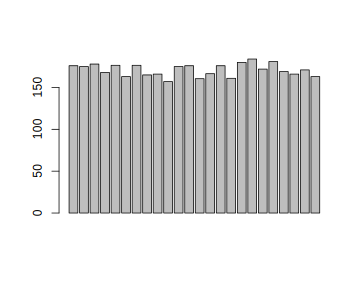
\includegraphics{Rprogramming_files/figure-latex/unnamed-chunk-8-1.pdf}

\begin{Shaded}
\begin{Highlighting}[]
\NormalTok{VADeaths}
\end{Highlighting}
\end{Shaded}

\begin{verbatim}
##       Rural Male Rural Female Urban Male Urban Female
## 50-54       11.7          8.7       15.4          8.4
## 55-59       18.1         11.7       24.3         13.6
## 60-64       26.9         20.3       37.0         19.3
## 65-69       41.0         30.9       54.6         35.1
## 70-74       66.0         54.3       71.1         50.0
\end{verbatim}

\begin{Shaded}
\begin{Highlighting}[]
\KeywordTok{barplot}\NormalTok{(VADeaths, }\DataTypeTok{border =} \StringTok{"dark blue"}\NormalTok{)}
\end{Highlighting}
\end{Shaded}

\includegraphics{Rprogramming_files/figure-latex/unnamed-chunk-8-2.pdf}

\begin{Shaded}
\begin{Highlighting}[]
\KeywordTok{barplot}\NormalTok{(VADeaths, }\DataTypeTok{col =} \KeywordTok{rainbow}\NormalTok{(}\DecValTok{20}\NormalTok{))}
\end{Highlighting}
\end{Shaded}

\includegraphics{Rprogramming_files/figure-latex/unnamed-chunk-8-3.pdf}

\begin{Shaded}
\begin{Highlighting}[]
\KeywordTok{barplot}\NormalTok{(VADeaths, }\DataTypeTok{col =} \KeywordTok{heat.colors}\NormalTok{(}\DecValTok{8}\NormalTok{))}
\end{Highlighting}
\end{Shaded}

\includegraphics{Rprogramming_files/figure-latex/unnamed-chunk-8-4.pdf}

\begin{Shaded}
\begin{Highlighting}[]
\KeywordTok{barplot}\NormalTok{(VADeaths, }\DataTypeTok{col =} \KeywordTok{gray.colors}\NormalTok{(}\DecValTok{4}\NormalTok{))}
\end{Highlighting}
\end{Shaded}

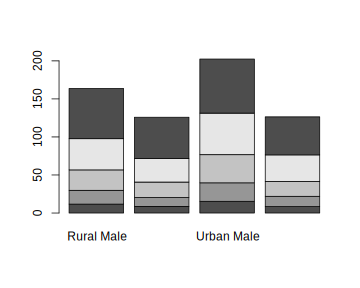
\includegraphics{Rprogramming_files/figure-latex/unnamed-chunk-8-5.pdf}

\begin{Shaded}
\begin{Highlighting}[]
\KeywordTok{barplot}\NormalTok{(VADeaths, }\DataTypeTok{col =} \KeywordTok{gray.colors}\NormalTok{(}\DecValTok{4}\NormalTok{), }\DataTypeTok{log=}\StringTok{"x"}\NormalTok{)}
\end{Highlighting}
\end{Shaded}

\includegraphics{Rprogramming_files/figure-latex/unnamed-chunk-8-6.pdf}

\begin{Shaded}
\begin{Highlighting}[]
\KeywordTok{barplot}\NormalTok{(VADeaths, }\DataTypeTok{col =} \KeywordTok{gray.colors}\NormalTok{(}\DecValTok{4}\NormalTok{), }\DataTypeTok{log=}\StringTok{"y"}\NormalTok{)}
\end{Highlighting}
\end{Shaded}

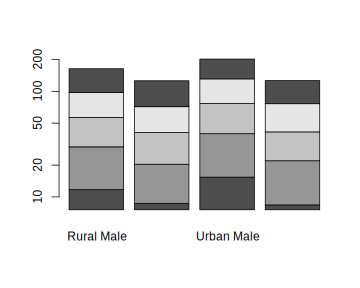
\includegraphics{Rprogramming_files/figure-latex/unnamed-chunk-8-7.pdf}

\begin{Shaded}
\begin{Highlighting}[]
\KeywordTok{barplot}\NormalTok{(VADeaths, }\DataTypeTok{col =} \KeywordTok{gray.colors}\NormalTok{(}\DecValTok{4}\NormalTok{), }\DataTypeTok{log=}\StringTok{"xy"}\NormalTok{)}
\end{Highlighting}
\end{Shaded}

\includegraphics{Rprogramming_files/figure-latex/unnamed-chunk-8-8.pdf}

\subsection{pie chart}\label{pie-chart}

\begin{Shaded}
\begin{Highlighting}[]
\NormalTok{drug.X.market <-}\StringTok{ }\KeywordTok{c}\NormalTok{(}\FloatTok{0.12}\NormalTok{, }\FloatTok{0.29}\NormalTok{, }\FloatTok{0.32}\NormalTok{, }\FloatTok{0.22}\NormalTok{, }\FloatTok{0.11}\NormalTok{, }\FloatTok{0.28}\NormalTok{)}
\KeywordTok{names}\NormalTok{(drug.X.market) <-}\StringTok{ }\KeywordTok{c}\NormalTok{(}\StringTok{"South Korea"}\NormalTok{,}\StringTok{"China"}\NormalTok{,}\StringTok{"USA"}\NormalTok{,}\StringTok{"Japan"}\NormalTok{,}\StringTok{"Austria"}\NormalTok{,}\StringTok{"EU"}\NormalTok{)}
\KeywordTok{pie}\NormalTok{(drug.X.market)}
\end{Highlighting}
\end{Shaded}

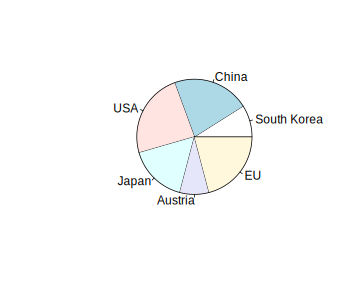
\includegraphics{Rprogramming_files/figure-latex/unnamed-chunk-9-1.pdf}

\subsection{matplot 함수}\label{matplot-}

\subsubsection{matrix와 column 사이의 그림}\label{matrix-column--}

\begin{Shaded}
\begin{Highlighting}[]
\NormalTok{pct.}\DecValTok{95}\NormalTok{ <-}\StringTok{ }\KeywordTok{read.csv}\NormalTok{(}\StringTok{"pct95.csv"}\NormalTok{)}
\KeywordTok{matplot}\NormalTok{(pct.}\DecValTok{95}\NormalTok{[,}\DecValTok{1}\NormalTok{], pct.}\DecValTok{95}\NormalTok{[,}\DecValTok{2}\OperatorTok{:}\KeywordTok{ncol}\NormalTok{(pct.}\DecValTok{95}\NormalTok{)], }\DataTypeTok{pch=}\DecValTok{1}\NormalTok{)}
\end{Highlighting}
\end{Shaded}

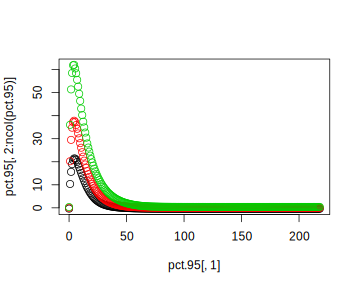
\includegraphics{Rprogramming_files/figure-latex/unnamed-chunk-10-1.pdf}

\begin{Shaded}
\begin{Highlighting}[]
\KeywordTok{matplot}\NormalTok{(pct.}\DecValTok{95}\NormalTok{[,}\DecValTok{1}\NormalTok{], pct.}\DecValTok{95}\NormalTok{[,}\DecValTok{2}\OperatorTok{:}\KeywordTok{ncol}\NormalTok{(pct.}\DecValTok{95}\NormalTok{)], }\DataTypeTok{pch=}\DecValTok{1}\NormalTok{, }\DataTypeTok{col=}\KeywordTok{c}\NormalTok{(}\DecValTok{1}\NormalTok{,}\DecValTok{2}\NormalTok{,}\DecValTok{1}\NormalTok{), }\DataTypeTok{type=}\StringTok{"l"}\NormalTok{, }\DataTypeTok{lty=}\DecValTok{1}\NormalTok{, }\DataTypeTok{lwd=}\KeywordTok{c}\NormalTok{(}\DecValTok{1}\NormalTok{,}\DecValTok{2}\NormalTok{,}\DecValTok{1}\NormalTok{))}
\end{Highlighting}
\end{Shaded}

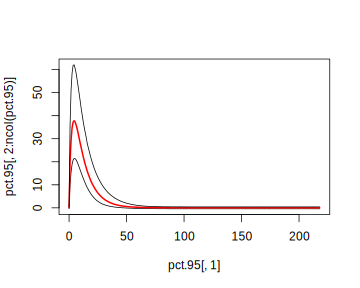
\includegraphics{Rprogramming_files/figure-latex/unnamed-chunk-10-2.pdf}

\subsection{Scatter plot matrices (pairs
plots)}\label{scatter-plot-matrices-pairs-plots}

\begin{Shaded}
\begin{Highlighting}[]
\KeywordTok{pairs}\NormalTok{(d.demog)}
\end{Highlighting}
\end{Shaded}

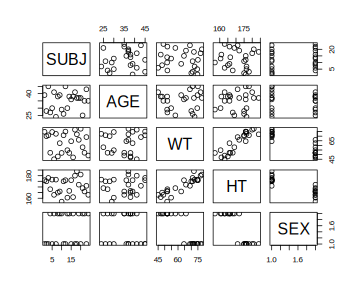
\includegraphics{Rprogramming_files/figure-latex/unnamed-chunk-11-1.pdf}

\subsubsection{add a loess smoother,
type}\label{add-a-loess-smoother-type}

\begin{Shaded}
\begin{Highlighting}[]
\KeywordTok{pairs}\NormalTok{(d.demog, }\DataTypeTok{panel =}\NormalTok{ panel.smooth)}
\end{Highlighting}
\end{Shaded}

\includegraphics{Rprogramming_files/figure-latex/unnamed-chunk-12-1.pdf}

\begin{Shaded}
\begin{Highlighting}[]
\NormalTok{panel.cor <-}\StringTok{ }\ControlFlowTok{function}\NormalTok{(x, y, }\DataTypeTok{digits=}\DecValTok{2}\NormalTok{, }\DataTypeTok{prefix=}\StringTok{""}\NormalTok{, cex.cor)}
\NormalTok{\{}
\NormalTok{    usr <-}\StringTok{ }\KeywordTok{par}\NormalTok{(}\StringTok{"usr"}\NormalTok{); }\KeywordTok{on.exit}\NormalTok{(}\KeywordTok{par}\NormalTok{(usr))}
    \KeywordTok{par}\NormalTok{(}\DataTypeTok{usr =} \KeywordTok{c}\NormalTok{(}\DecValTok{0}\NormalTok{, }\DecValTok{1}\NormalTok{, }\DecValTok{0}\NormalTok{, }\DecValTok{1}\NormalTok{))}
\NormalTok{    r =}\StringTok{ }\NormalTok{(}\KeywordTok{cor}\NormalTok{(x, y))}
\NormalTok{    txt <-}\StringTok{ }\KeywordTok{format}\NormalTok{(}\KeywordTok{c}\NormalTok{(r, }\FloatTok{0.123456789}\NormalTok{), }\DataTypeTok{digits=}\NormalTok{digits)[}\DecValTok{1}\NormalTok{]}
\NormalTok{    txt <-}\StringTok{ }\KeywordTok{paste}\NormalTok{(prefix, txt, }\DataTypeTok{sep=}\StringTok{""}\NormalTok{)}
    \ControlFlowTok{if}\NormalTok{(}\KeywordTok{missing}\NormalTok{(cex.cor)) cex <-}\StringTok{ }\FloatTok{1.5}
    \KeywordTok{text}\NormalTok{(}\FloatTok{0.5}\NormalTok{, }\FloatTok{0.5}\NormalTok{, txt, }\DataTypeTok{cex =} \FloatTok{1.5}\NormalTok{)}
\NormalTok{\}}

\KeywordTok{pairs}\NormalTok{(d.demog, }\DataTypeTok{lower.panel=}\NormalTok{panel.smooth, }\DataTypeTok{upper.panel=}\NormalTok{panel.cor) }
\end{Highlighting}
\end{Shaded}

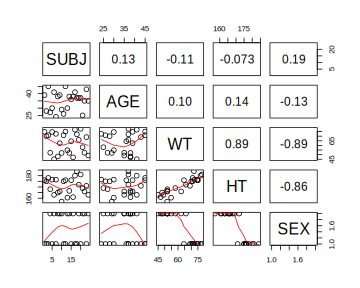
\includegraphics{Rprogramming_files/figure-latex/unnamed-chunk-12-2.pdf}

\section{하위수준 그림 함수}\label{lower}

\begin{itemize}
\tightlist
\item
  points : 점추가
\item
  lines : 선 추가
\item
  abline : 기준선 추가
\item
  mtext : 텍스트 추가
\item
  legend : 설명(legend) 추가
\item
  polygon : polygon 추가
\end{itemize}

\subsection{점, 선, 설명 추가 하기 \{add\}}\label{-----add}

\begin{Shaded}
\begin{Highlighting}[]
\KeywordTok{plot}\NormalTok{(pct.}\DecValTok{95}\OperatorTok{$}\NormalTok{TIME, pct.}\DecValTok{95}\OperatorTok{$}\NormalTok{PCT50, }\DataTypeTok{main=}\StringTok{"PK of Drug X"}
\NormalTok{     , }\DataTypeTok{type=}\StringTok{"l"}\NormalTok{, }\DataTypeTok{xlab=}\StringTok{"Time (h)"}\NormalTok{, }\DataTypeTok{ylab=}\StringTok{"Concentration (ng/ml)"}
\NormalTok{     , }\DataTypeTok{ylim=}\KeywordTok{range}\NormalTok{(}\DecValTok{0}\NormalTok{,}\DecValTok{80}\NormalTok{), }\DataTypeTok{lty=}\DecValTok{1}\NormalTok{, }\DataTypeTok{col=}\StringTok{"red"}\NormalTok{, }\DataTypeTok{lwd=}\DecValTok{2}\NormalTok{)}
\end{Highlighting}
\end{Shaded}

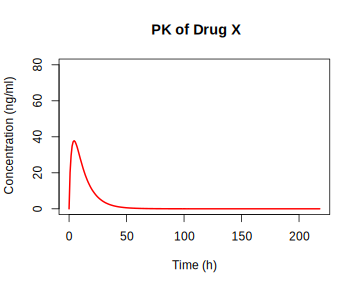
\includegraphics{Rprogramming_files/figure-latex/unnamed-chunk-13-1.pdf}

\begin{Shaded}
\begin{Highlighting}[]
\KeywordTok{plot}\NormalTok{(dta}\OperatorTok{$}\NormalTok{TIME[dta}\OperatorTok{$}\NormalTok{MDV}\OperatorTok{==}\DecValTok{0}\NormalTok{], dta}\OperatorTok{$}\NormalTok{DV[dta}\OperatorTok{$}\NormalTok{MDV}\OperatorTok{==}\DecValTok{0}\NormalTok{], }\DataTypeTok{main=}\StringTok{"PK of Drug X"}
\NormalTok{     , }\DataTypeTok{type=}\StringTok{"n"}\NormalTok{, }\DataTypeTok{xlab=}\StringTok{"Time (h)"}\NormalTok{, }\DataTypeTok{ylab=}\StringTok{"Concentration (ng/ml)"}
\NormalTok{     , }\DataTypeTok{ylim=}\KeywordTok{range}\NormalTok{(}\DecValTok{0}\NormalTok{,}\DecValTok{80}\NormalTok{))}
\KeywordTok{points}\NormalTok{(dta}\OperatorTok{$}\NormalTok{TIME[dta}\OperatorTok{$}\NormalTok{MDV}\OperatorTok{==}\DecValTok{0}\NormalTok{], dta}\OperatorTok{$}\NormalTok{DV[dta}\OperatorTok{$}\NormalTok{MDV}\OperatorTok{==}\DecValTok{0}\NormalTok{], }\DataTypeTok{pch =} \DecValTok{16}\NormalTok{, }\DataTypeTok{cex=}\FloatTok{0.8}\NormalTok{)}
\KeywordTok{lines}\NormalTok{(dta}\OperatorTok{$}\NormalTok{TIME[dta}\OperatorTok{$}\NormalTok{MDV}\OperatorTok{==}\DecValTok{0}\NormalTok{], dta}\OperatorTok{$}\NormalTok{DV[dta}\OperatorTok{$}\NormalTok{MDV}\OperatorTok{==}\DecValTok{0}\NormalTok{], }\DataTypeTok{col=}\StringTok{"black"}\NormalTok{, }\DataTypeTok{lwd=}\DecValTok{1}\NormalTok{)}
\KeywordTok{abline}\NormalTok{(}\DecValTok{40}\NormalTok{, }\DecValTok{0}\NormalTok{, }\DataTypeTok{col=}\StringTok{"red"}\NormalTok{, }\DataTypeTok{lty=}\DecValTok{2}\NormalTok{)                               }\CommentTok{# abline(a,b): y=a+b*x}
\KeywordTok{legend}\NormalTok{(}\StringTok{"topright"}\NormalTok{, }\DataTypeTok{legend=}\KeywordTok{c}\NormalTok{(}\StringTok{"Individual concentrations"}\NormalTok{)}
\NormalTok{       , }\DataTypeTok{lty=}\DecValTok{1}\NormalTok{, }\DataTypeTok{col=}\StringTok{"black"}\NormalTok{)}
\end{Highlighting}
\end{Shaded}

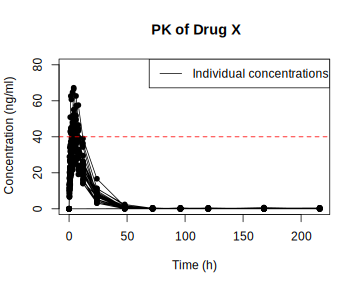
\includegraphics{Rprogramming_files/figure-latex/unnamed-chunk-13-2.pdf}

\subsection{polygon 함수}\label{polygon-}

\begin{Shaded}
\begin{Highlighting}[]
\KeywordTok{plot}\NormalTok{(}\KeywordTok{c}\NormalTok{(}\DecValTok{1}\NormalTok{, }\DecValTok{10}\NormalTok{), }\KeywordTok{c}\NormalTok{(}\DecValTok{1}\NormalTok{, }\DecValTok{6}\NormalTok{), }\DataTypeTok{type =} \StringTok{"n"}\NormalTok{)}
\KeywordTok{polygon}\NormalTok{(}\KeywordTok{c}\NormalTok{(}\DecValTok{2}\NormalTok{,}\DecValTok{8}\NormalTok{,}\DecValTok{8}\NormalTok{,}\DecValTok{2}\NormalTok{), }\KeywordTok{c}\NormalTok{(}\DecValTok{5}\NormalTok{,}\DecValTok{4}\NormalTok{,}\DecValTok{3}\NormalTok{,}\DecValTok{2}\NormalTok{), }\DataTypeTok{col=}\StringTok{"lightgreen"}\NormalTok{)}
\end{Highlighting}
\end{Shaded}

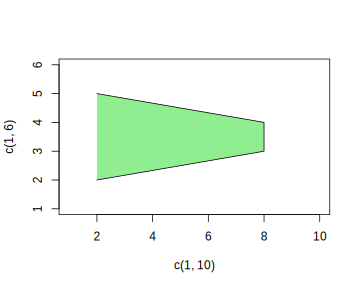
\includegraphics{Rprogramming_files/figure-latex/unnamed-chunk-14-1.pdf}

\begin{Shaded}
\begin{Highlighting}[]
\KeywordTok{plot}\NormalTok{(}\KeywordTok{c}\NormalTok{(}\DecValTok{1}\NormalTok{, }\DecValTok{9}\NormalTok{), }\DecValTok{1}\OperatorTok{:}\DecValTok{2}\NormalTok{, }\DataTypeTok{type =} \StringTok{"n"}\NormalTok{)}
\KeywordTok{polygon}\NormalTok{(}\DecValTok{1}\OperatorTok{:}\DecValTok{9}\NormalTok{, }\KeywordTok{c}\NormalTok{(}\DecValTok{2}\NormalTok{,}\DecValTok{1}\NormalTok{,}\DecValTok{2}\NormalTok{,}\DecValTok{1}\NormalTok{,}\DecValTok{1}\NormalTok{,}\DecValTok{2}\NormalTok{,}\DecValTok{1}\NormalTok{,}\DecValTok{2}\NormalTok{,}\DecValTok{1}\NormalTok{),}
        \DataTypeTok{col =} \KeywordTok{c}\NormalTok{(}\StringTok{"red"}\NormalTok{, }\StringTok{"blue"}\NormalTok{),}
        \DataTypeTok{border =} \KeywordTok{c}\NormalTok{(}\StringTok{"green"}\NormalTok{, }\StringTok{"yellow"}\NormalTok{),}
        \DataTypeTok{lwd =} \DecValTok{3}\NormalTok{, }\DataTypeTok{lty =} \KeywordTok{c}\NormalTok{(}\StringTok{"dashed"}\NormalTok{, }\StringTok{"solid"}\NormalTok{))}
\end{Highlighting}
\end{Shaded}

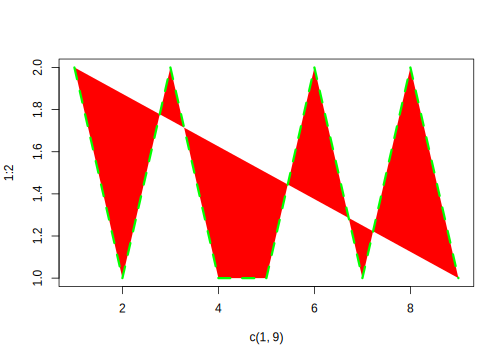
\includegraphics{Rprogramming_files/figure-latex/unnamed-chunk-14-2.pdf}

\section{그림 출력하기}\label{print}

\subsection{pdf graphics devices}\label{pdf-graphics-devices}

\begin{Shaded}
\begin{Highlighting}[]
\KeywordTok{pdf}\NormalTok{(}\StringTok{"PK_of_Drug_X.pdf"}\NormalTok{)}

\KeywordTok{plot}\NormalTok{(dta}\OperatorTok{$}\NormalTok{TIME[dta}\OperatorTok{$}\NormalTok{MDV}\OperatorTok{==}\DecValTok{0}\NormalTok{], dta}\OperatorTok{$}\NormalTok{DV[dta}\OperatorTok{$}\NormalTok{MDV}\OperatorTok{==}\DecValTok{0}\NormalTok{], }\DataTypeTok{main=}\StringTok{"PK of Drug X"}
\NormalTok{     , }\DataTypeTok{type=}\StringTok{"n"}\NormalTok{, }\DataTypeTok{xlab=}\StringTok{"Time (h)"}\NormalTok{, }\DataTypeTok{ylab=}\StringTok{"Concentration (ng/ml)"}
\NormalTok{     , }\DataTypeTok{ylim=}\KeywordTok{range}\NormalTok{(}\DecValTok{0}\NormalTok{,}\DecValTok{80}\NormalTok{))}
\KeywordTok{points}\NormalTok{(dta}\OperatorTok{$}\NormalTok{TIME[dta}\OperatorTok{$}\NormalTok{MDV}\OperatorTok{==}\DecValTok{0}\NormalTok{], dta}\OperatorTok{$}\NormalTok{DV[dta}\OperatorTok{$}\NormalTok{MDV}\OperatorTok{==}\DecValTok{0}\NormalTok{], }\DataTypeTok{pch =} \DecValTok{16}\NormalTok{, }\DataTypeTok{cex=}\FloatTok{0.8}\NormalTok{)}
\KeywordTok{lines}\NormalTok{(dta}\OperatorTok{$}\NormalTok{TIME[dta}\OperatorTok{$}\NormalTok{MDV}\OperatorTok{==}\DecValTok{0}\NormalTok{], dta}\OperatorTok{$}\NormalTok{DV[dta}\OperatorTok{$}\NormalTok{MDV}\OperatorTok{==}\DecValTok{0}\NormalTok{], }\DataTypeTok{col=}\StringTok{"black"}\NormalTok{, }\DataTypeTok{lwd=}\DecValTok{1}\NormalTok{)}
\KeywordTok{abline}\NormalTok{(}\DecValTok{40}\NormalTok{, }\DecValTok{0}\NormalTok{, }\DataTypeTok{col=}\StringTok{"red"}\NormalTok{, }\DataTypeTok{lty=}\DecValTok{2}\NormalTok{)                               }\CommentTok{#abline(a,b): y=a+b*x}
\KeywordTok{legend}\NormalTok{(}\StringTok{"topright"}\NormalTok{, }\DataTypeTok{legend=}\KeywordTok{c}\NormalTok{(}\StringTok{"Individual concentrations"}\NormalTok{)}
\NormalTok{       , }\DataTypeTok{lty=}\DecValTok{1}\NormalTok{, }\DataTypeTok{col=}\StringTok{"black"}\NormalTok{)}

\KeywordTok{dev.off}\NormalTok{()}
\end{Highlighting}
\end{Shaded}

\begin{verbatim}
## cairo_pdf 
##         2
\end{verbatim}

\subsection{PNG graphics devices}\label{png-graphics-devices}

\begin{Shaded}
\begin{Highlighting}[]
\KeywordTok{png}\NormalTok{(}\StringTok{"PK_of_Drug_X.png"}\NormalTok{)}

\KeywordTok{plot}\NormalTok{(dta}\OperatorTok{$}\NormalTok{TIME[dta}\OperatorTok{$}\NormalTok{MDV}\OperatorTok{==}\DecValTok{0}\NormalTok{], dta}\OperatorTok{$}\NormalTok{DV[dta}\OperatorTok{$}\NormalTok{MDV}\OperatorTok{==}\DecValTok{0}\NormalTok{], }\DataTypeTok{main=}\StringTok{"PK of Drug X"}
\NormalTok{     , }\DataTypeTok{type=}\StringTok{"n"}\NormalTok{, }\DataTypeTok{xlab=}\StringTok{"Time (h)"}\NormalTok{, }\DataTypeTok{ylab=}\StringTok{"Concentration (ng/ml)"}
\NormalTok{     , }\DataTypeTok{ylim=}\KeywordTok{range}\NormalTok{(}\DecValTok{0}\NormalTok{,}\DecValTok{80}\NormalTok{))}
\KeywordTok{points}\NormalTok{(dta}\OperatorTok{$}\NormalTok{TIME[dta}\OperatorTok{$}\NormalTok{MDV}\OperatorTok{==}\DecValTok{0}\NormalTok{], dta}\OperatorTok{$}\NormalTok{DV[dta}\OperatorTok{$}\NormalTok{MDV}\OperatorTok{==}\DecValTok{0}\NormalTok{], }\DataTypeTok{pch =} \DecValTok{16}\NormalTok{, }\DataTypeTok{cex=}\FloatTok{0.8}\NormalTok{)}
\KeywordTok{lines}\NormalTok{(dta}\OperatorTok{$}\NormalTok{TIME[dta}\OperatorTok{$}\NormalTok{MDV}\OperatorTok{==}\DecValTok{0}\NormalTok{], dta}\OperatorTok{$}\NormalTok{DV[dta}\OperatorTok{$}\NormalTok{MDV}\OperatorTok{==}\DecValTok{0}\NormalTok{], }\DataTypeTok{col=}\StringTok{"black"}\NormalTok{, }\DataTypeTok{lwd=}\DecValTok{1}\NormalTok{)}
\KeywordTok{abline}\NormalTok{(}\DecValTok{40}\NormalTok{, }\DecValTok{0}\NormalTok{, }\DataTypeTok{col=}\StringTok{"red"}\NormalTok{, }\DataTypeTok{lty=}\DecValTok{2}\NormalTok{)                               }\CommentTok{#abline(a,b): y=a+b*x}
\KeywordTok{legend}\NormalTok{(}\StringTok{"topright"}\NormalTok{, }\DataTypeTok{legend=}\KeywordTok{c}\NormalTok{(}\StringTok{"Individual concentrations"}\NormalTok{)}
\NormalTok{       , }\DataTypeTok{lty=}\DecValTok{1}\NormalTok{, }\DataTypeTok{col=}\StringTok{"black"}\NormalTok{)}

\KeywordTok{dev.off}\NormalTok{()}
\end{Highlighting}
\end{Shaded}

\begin{verbatim}
## cairo_pdf 
##         2
\end{verbatim}

\chapter{Data Import / Export}\label{data-import-export}

\begin{quote}
2017-03-29 배균섭 교수님 강의
\end{quote}

이번 시간에는 자료를 불러오고 조작을 가한 뒤 저장하는 방법에 대해
알아보겠습니다.

\section{Read.csv}\label{read.csv}

\texttt{setwd} 명령어를 통해서 자료가 있는 작업 공간을 설정할 수
있습니다. 설정 후에서는 \texttt{dir()}을 통해 파일의 이름을 확인 할 수
있습니다. \texttt{read.csv}를 통해서 자료를 R에서 사용할 수 있게 됩니다.

\begin{Shaded}
\begin{Highlighting}[]
\KeywordTok{setwd}\NormalTok{(}\StringTok{"D:/Rt"}\NormalTok{)}
\KeywordTok{dir}\NormalTok{()}
\NormalTok{mydata <-}\StringTok{ }\KeywordTok{read.csv}\NormalTok{(}\StringTok{"MyData2017.csv"}\NormalTok{, }\DataTypeTok{as.is=}\OtherTok{TRUE}\NormalTok{)}
\end{Highlighting}
\end{Shaded}

\section{Theoph 데이타}\label{theoph-}

R에 기본적으로 들어있는 \texttt{Theoph} 약동학 자료에 대해
살펴보겠습니다.

\begin{Shaded}
\begin{Highlighting}[]
\KeywordTok{head}\NormalTok{(Theoph, }\DataTypeTok{n =} \DecValTok{11}\NormalTok{)}
\end{Highlighting}
\end{Shaded}

\begin{verbatim}
##    Subject   Wt Dose  Time  conc
## 1        1 79.6 4.02  0.00  0.74
## 2        1 79.6 4.02  0.25  2.84
## 3        1 79.6 4.02  0.57  6.57
## 4        1 79.6 4.02  1.12 10.50
## 5        1 79.6 4.02  2.02  9.66
## 6        1 79.6 4.02  3.82  8.58
## 7        1 79.6 4.02  5.10  8.36
## 8        1 79.6 4.02  7.03  7.47
## 9        1 79.6 4.02  9.05  6.89
## 10       1 79.6 4.02 12.12  5.94
## 11       1 79.6 4.02 24.37  3.28
\end{verbatim}

\begin{Shaded}
\begin{Highlighting}[]
\KeywordTok{tail}\NormalTok{(Theoph, }\DataTypeTok{n =} \DecValTok{11}\NormalTok{)}
\end{Highlighting}
\end{Shaded}

\begin{verbatim}
##     Subject   Wt Dose  Time conc
## 122      12 60.5  5.3  0.00 0.00
## 123      12 60.5  5.3  0.25 1.25
## 124      12 60.5  5.3  0.50 3.96
## 125      12 60.5  5.3  1.00 7.82
## 126      12 60.5  5.3  2.00 9.72
## 127      12 60.5  5.3  3.52 9.75
## 128      12 60.5  5.3  5.07 8.57
## 129      12 60.5  5.3  7.07 6.59
## 130      12 60.5  5.3  9.03 6.11
## 131      12 60.5  5.3 12.05 4.57
## 132      12 60.5  5.3 24.15 1.17
\end{verbatim}

R console에서 \texttt{?Theoph}를 타이핑 치면 좀 더 자세한 정보를 얻을 수
있습니다.

\section{lattice}\label{lattice}

lattice 패키지를 불러온 뒤 그림을 그려보겠습니다. \citep{R-lattice}
\index{lattice}

\begin{Shaded}
\begin{Highlighting}[]
\KeywordTok{library}\NormalTok{(lattice) }\CommentTok{# trellis}

\KeywordTok{xyplot}\NormalTok{(conc }\OperatorTok{~}\StringTok{ }\NormalTok{Time }\OperatorTok{|}\StringTok{ }\NormalTok{Subject, }\DataTypeTok{data=}\NormalTok{Theoph)}
\end{Highlighting}
\end{Shaded}

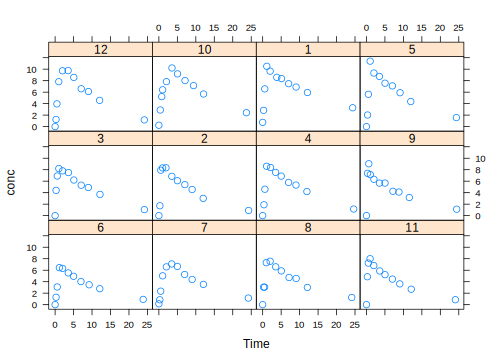
\includegraphics{Rprogramming_files/figure-latex/unnamed-chunk-19-1.pdf}

\begin{Shaded}
\begin{Highlighting}[]
\KeywordTok{xyplot}\NormalTok{(conc }\OperatorTok{~}\StringTok{ }\NormalTok{Time }\OperatorTok{|}\StringTok{ }\NormalTok{Subject, }\DataTypeTok{data=}\NormalTok{Theoph, }\DataTypeTok{type=}\StringTok{"b"}\NormalTok{)}
\end{Highlighting}
\end{Shaded}

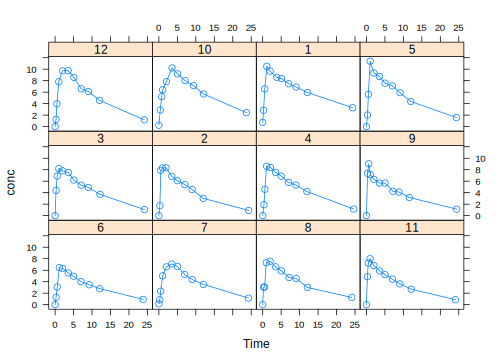
\includegraphics{Rprogramming_files/figure-latex/unnamed-chunk-19-2.pdf}

\begin{Shaded}
\begin{Highlighting}[]
\NormalTok{Theoph[,}\StringTok{"ID"}\NormalTok{] =}\StringTok{ }\KeywordTok{as.numeric}\NormalTok{(}\KeywordTok{as.character}\NormalTok{(Theoph[,}\StringTok{"Subject"}\NormalTok{]))}

\KeywordTok{xyplot}\NormalTok{(conc }\OperatorTok{~}\StringTok{ }\NormalTok{Time }\OperatorTok{|}\StringTok{ }\NormalTok{ID, }\DataTypeTok{data=}\NormalTok{Theoph, }\DataTypeTok{type=}\StringTok{"b"}\NormalTok{)}
\end{Highlighting}
\end{Shaded}

\includegraphics{Rprogramming_files/figure-latex/unnamed-chunk-19-3.pdf}

\begin{Shaded}
\begin{Highlighting}[]
\KeywordTok{xyplot}\NormalTok{(conc }\OperatorTok{~}\StringTok{ }\NormalTok{Time }\OperatorTok{|}\StringTok{ }\KeywordTok{as.factor}\NormalTok{(ID), }\DataTypeTok{data=}\NormalTok{Theoph, }\DataTypeTok{type=}\StringTok{"b"}\NormalTok{)}
\end{Highlighting}
\end{Shaded}

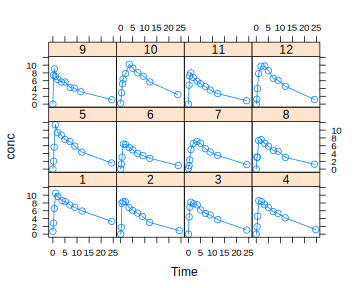
\includegraphics{Rprogramming_files/figure-latex/unnamed-chunk-19-4.pdf}

\begin{Shaded}
\begin{Highlighting}[]
\KeywordTok{write.csv}\NormalTok{(Theoph, }\StringTok{"Theoph.csv"}\NormalTok{, }\DataTypeTok{row.names=}\OtherTok{FALSE}\NormalTok{, }\DataTypeTok{quote=}\OtherTok{FALSE}\NormalTok{, }\DataTypeTok{na=}\StringTok{""}\NormalTok{)}
\end{Highlighting}
\end{Shaded}

\section{Subseting and write.csv}\label{subseting-and-write.csv}

자료를 편집하고, subset을 만들고 각각을 파일로 저장하는 방법에 대해
알아보겠습니다.

\begin{Shaded}
\begin{Highlighting}[]
\NormalTok{IDs =}\StringTok{ }\KeywordTok{sort}\NormalTok{(}\KeywordTok{unique}\NormalTok{(Theoph[,}\StringTok{"ID"}\NormalTok{])) ; IDs}
\end{Highlighting}
\end{Shaded}

\begin{verbatim}
##  [1]  1  2  3  4  5  6  7  8  9 10 11 12
\end{verbatim}

\begin{Shaded}
\begin{Highlighting}[]
\NormalTok{nID =}\StringTok{ }\KeywordTok{length}\NormalTok{(IDs) ; nID}
\end{Highlighting}
\end{Shaded}

\begin{verbatim}
## [1] 12
\end{verbatim}

\begin{Shaded}
\begin{Highlighting}[]
\NormalTok{demog =}\StringTok{ }\KeywordTok{unique}\NormalTok{(Theoph[,}\KeywordTok{c}\NormalTok{(}\StringTok{"ID"}\NormalTok{,}\StringTok{"Wt"}\NormalTok{)])}
\KeywordTok{colnames}\NormalTok{(demog) =}\StringTok{ }\KeywordTok{c}\NormalTok{(}\StringTok{"ID"}\NormalTok{, }\StringTok{"BWT"}\NormalTok{)}
\KeywordTok{write.csv}\NormalTok{(demog, }\StringTok{"1-demog.csv"}\NormalTok{, }\DataTypeTok{row.names=}\OtherTok{FALSE}\NormalTok{, }\DataTypeTok{quote=}\OtherTok{FALSE}\NormalTok{, }\DataTypeTok{na=}\StringTok{""}\NormalTok{)}

\NormalTok{DV =}\StringTok{ }\NormalTok{Theoph[,}\KeywordTok{c}\NormalTok{(}\StringTok{"ID"}\NormalTok{,}\StringTok{"Time"}\NormalTok{, }\StringTok{"conc"}\NormalTok{)]}
\KeywordTok{colnames}\NormalTok{(DV) =}\StringTok{ }\KeywordTok{c}\NormalTok{(}\StringTok{"ID"}\NormalTok{, }\StringTok{"TIME"}\NormalTok{, }\StringTok{"DV"}\NormalTok{)}
\KeywordTok{write.csv}\NormalTok{(DV, }\StringTok{"3-DV.csv"}\NormalTok{, }\DataTypeTok{row.names=}\OtherTok{FALSE}\NormalTok{, }\DataTypeTok{quote=}\OtherTok{FALSE}\NormalTok{, }\DataTypeTok{na=}\StringTok{""}\NormalTok{)}

\NormalTok{adm =}\StringTok{ }\KeywordTok{cbind}\NormalTok{(IDs, }\KeywordTok{rep}\NormalTok{(}\DecValTok{0}\NormalTok{, nID), }\KeywordTok{rep}\NormalTok{(}\DecValTok{320}\NormalTok{, nID))}
\KeywordTok{colnames}\NormalTok{(adm) =}\StringTok{ }\KeywordTok{c}\NormalTok{(}\StringTok{"ID"}\NormalTok{, }\StringTok{"TIME"}\NormalTok{, }\StringTok{"AMT"}\NormalTok{)}
\KeywordTok{write.csv}\NormalTok{(adm, }\StringTok{"2-adm.csv"}\NormalTok{, }\DataTypeTok{row.names=}\OtherTok{FALSE}\NormalTok{, }\DataTypeTok{quote=}\OtherTok{FALSE}\NormalTok{, }\DataTypeTok{na=}\StringTok{""}\NormalTok{)}

\NormalTok{demog =}\StringTok{ }\KeywordTok{read.csv}\NormalTok{(}\StringTok{"1-demog.csv"}\NormalTok{, }\DataTypeTok{as.is=}\OtherTok{TRUE}\NormalTok{)}
\NormalTok{adm =}\StringTok{ }\KeywordTok{read.csv}\NormalTok{(}\StringTok{"2-adm.csv"}\NormalTok{, }\DataTypeTok{as.is=}\OtherTok{TRUE}\NormalTok{)}
\NormalTok{dv =}\StringTok{ }\KeywordTok{read.csv}\NormalTok{(}\StringTok{"3-dv.csv"}\NormalTok{, }\DataTypeTok{as.is=}\OtherTok{TRUE}\NormalTok{)}

\NormalTok{AdmDv =}\StringTok{ }\KeywordTok{merge}\NormalTok{(adm, dv, }\DataTypeTok{by=}\KeywordTok{intersect}\NormalTok{(}\KeywordTok{colnames}\NormalTok{(adm), }\KeywordTok{colnames}\NormalTok{(dv)), }\DataTypeTok{all=}\OtherTok{TRUE}\NormalTok{)}
\NormalTok{AdmDv}
\end{Highlighting}
\end{Shaded}

\begin{verbatim}
##     ID  TIME AMT    DV
## 1    1  0.00 320  0.74
## 2    1  0.25  NA  2.84
## 3    1  0.57  NA  6.57
## 4    1  1.12  NA 10.50
## 5    1  2.02  NA  9.66
## 6    1  3.82  NA  8.58
## 7    1  5.10  NA  8.36
## 8    1  7.03  NA  7.47
## 9    1  9.05  NA  6.89
## 10   1 12.12  NA  5.94
## 11   1 24.37  NA  3.28
## 12   2  0.00 320  0.00
## 13   2  0.27  NA  1.72
## 14   2  0.52  NA  7.91
## 15   2  1.00  NA  8.31
## 16   2  1.92  NA  8.33
## 17   2  3.50  NA  6.85
## 18   2  5.02  NA  6.08
## 19   2  7.03  NA  5.40
## 20   2  9.00  NA  4.55
## 21   2 12.00  NA  3.01
## 22   2 24.30  NA  0.90
## 23   3  0.00 320  0.00
## 24   3  0.27  NA  4.40
## 25   3  0.58  NA  6.90
## 26   3  1.02  NA  8.20
## 27   3  2.02  NA  7.80
## 28   3  3.62  NA  7.50
## 29   3  5.08  NA  6.20
## 30   3  7.07  NA  5.30
## 31   3  9.00  NA  4.90
## 32   3 12.15  NA  3.70
## 33   3 24.17  NA  1.05
## 34   4  0.00 320  0.00
## 35   4  0.35  NA  1.89
## 36   4  0.60  NA  4.60
## 37   4  1.07  NA  8.60
## 38   4  2.13  NA  8.38
## 39   4  3.50  NA  7.54
## 40   4  5.02  NA  6.88
## 41   4  7.02  NA  5.78
## 42   4  9.02  NA  5.33
## 43   4 11.98  NA  4.19
## 44   4 24.65  NA  1.15
## 45   5  0.00 320  0.00
## 46   5  0.30  NA  2.02
## 47   5  0.52  NA  5.63
## 48   5  1.00  NA 11.40
## 49   5  2.02  NA  9.33
## 50   5  3.50  NA  8.74
## 51   5  5.02  NA  7.56
## 52   5  7.02  NA  7.09
## 53   5  9.10  NA  5.90
## 54   5 12.00  NA  4.37
## 55   5 24.35  NA  1.57
## 56   6  0.00 320  0.00
## 57   6  0.27  NA  1.29
## 58   6  0.58  NA  3.08
## 59   6  1.15  NA  6.44
## 60   6  2.03  NA  6.32
## 61   6  3.57  NA  5.53
## 62   6  5.00  NA  4.94
## 63   6  7.00  NA  4.02
## 64   6  9.22  NA  3.46
## 65   6 12.10  NA  2.78
## 66   6 23.85  NA  0.92
## 67   7  0.00 320  0.15
## 68   7  0.25  NA  0.85
## 69   7  0.50  NA  2.35
## 70   7  1.02  NA  5.02
## 71   7  2.02  NA  6.58
## 72   7  3.48  NA  7.09
## 73   7  5.00  NA  6.66
## 74   7  6.98  NA  5.25
## 75   7  9.00  NA  4.39
## 76   7 12.05  NA  3.53
## 77   7 24.22  NA  1.15
## 78   8  0.00 320  0.00
## 79   8  0.25  NA  3.05
## 80   8  0.52  NA  3.05
## 81   8  0.98  NA  7.31
## 82   8  2.02  NA  7.56
## 83   8  3.53  NA  6.59
## 84   8  5.05  NA  5.88
## 85   8  7.15  NA  4.73
## 86   8  9.07  NA  4.57
## 87   8 12.10  NA  3.00
## 88   8 24.12  NA  1.25
## 89   9  0.00 320  0.00
## 90   9  0.30  NA  7.37
## 91   9  0.63  NA  9.03
## 92   9  1.05  NA  7.14
## 93   9  2.02  NA  6.33
## 94   9  3.53  NA  5.66
## 95   9  5.02  NA  5.67
## 96   9  7.17  NA  4.24
## 97   9  8.80  NA  4.11
## 98   9 11.60  NA  3.16
## 99   9 24.43  NA  1.12
## 100 10  0.00 320  0.24
## 101 10  0.37  NA  2.89
## 102 10  0.77  NA  5.22
## 103 10  1.02  NA  6.41
## 104 10  2.05  NA  7.83
## 105 10  3.55  NA 10.21
## 106 10  5.05  NA  9.18
## 107 10  7.08  NA  8.02
## 108 10  9.38  NA  7.14
## 109 10 12.10  NA  5.68
## 110 10 23.70  NA  2.42
## 111 11  0.00 320  0.00
## 112 11  0.25  NA  4.86
## 113 11  0.50  NA  7.24
## 114 11  0.98  NA  8.00
## 115 11  1.98  NA  6.81
## 116 11  3.60  NA  5.87
## 117 11  5.02  NA  5.22
## 118 11  7.03  NA  4.45
## 119 11  9.03  NA  3.62
## 120 11 12.12  NA  2.69
## 121 11 24.08  NA  0.86
## 122 12  0.00 320  0.00
## 123 12  0.25  NA  1.25
## 124 12  0.50  NA  3.96
## 125 12  1.00  NA  7.82
## 126 12  2.00  NA  9.72
## 127 12  3.52  NA  9.75
## 128 12  5.07  NA  8.57
## 129 12  7.07  NA  6.59
## 130 12  9.03  NA  6.11
## 131 12 12.05  NA  4.57
## 132 12 24.15  NA  1.17
\end{verbatim}

자료를 병합(\texttt{merge})해 보겠습니다.

\begin{Shaded}
\begin{Highlighting}[]
\NormalTok{DataAll =}\StringTok{ }\KeywordTok{merge}\NormalTok{(demog, AdmDv, }\DataTypeTok{by=}\KeywordTok{c}\NormalTok{(}\StringTok{"ID"}\NormalTok{), }\DataTypeTok{all=}\OtherTok{TRUE}\NormalTok{)}
\NormalTok{DataAll}
\end{Highlighting}
\end{Shaded}

\begin{verbatim}
##     ID  BWT  TIME AMT    DV
## 1    1 79.6  0.00 320  0.74
## 2    1 79.6  0.25  NA  2.84
## 3    1 79.6  0.57  NA  6.57
## 4    1 79.6  1.12  NA 10.50
## 5    1 79.6  2.02  NA  9.66
## 6    1 79.6  3.82  NA  8.58
## 7    1 79.6  5.10  NA  8.36
## 8    1 79.6  7.03  NA  7.47
## 9    1 79.6  9.05  NA  6.89
## 10   1 79.6 12.12  NA  5.94
## 11   1 79.6 24.37  NA  3.28
## 12   2 72.4  0.00 320  0.00
## 13   2 72.4  0.27  NA  1.72
## 14   2 72.4  0.52  NA  7.91
## 15   2 72.4  1.00  NA  8.31
## 16   2 72.4  1.92  NA  8.33
## 17   2 72.4  3.50  NA  6.85
## 18   2 72.4  5.02  NA  6.08
## 19   2 72.4  7.03  NA  5.40
## 20   2 72.4  9.00  NA  4.55
## 21   2 72.4 12.00  NA  3.01
## 22   2 72.4 24.30  NA  0.90
## 23   3 70.5  0.00 320  0.00
## 24   3 70.5  0.27  NA  4.40
## 25   3 70.5  0.58  NA  6.90
## 26   3 70.5  1.02  NA  8.20
## 27   3 70.5  2.02  NA  7.80
## 28   3 70.5  3.62  NA  7.50
## 29   3 70.5  5.08  NA  6.20
## 30   3 70.5  7.07  NA  5.30
## 31   3 70.5  9.00  NA  4.90
## 32   3 70.5 12.15  NA  3.70
## 33   3 70.5 24.17  NA  1.05
## 34   4 72.7  0.00 320  0.00
## 35   4 72.7  0.35  NA  1.89
## 36   4 72.7  0.60  NA  4.60
## 37   4 72.7  1.07  NA  8.60
## 38   4 72.7  2.13  NA  8.38
## 39   4 72.7  3.50  NA  7.54
## 40   4 72.7  5.02  NA  6.88
## 41   4 72.7  7.02  NA  5.78
## 42   4 72.7  9.02  NA  5.33
## 43   4 72.7 11.98  NA  4.19
## 44   4 72.7 24.65  NA  1.15
## 45   5 54.6  0.00 320  0.00
## 46   5 54.6  0.30  NA  2.02
## 47   5 54.6  0.52  NA  5.63
## 48   5 54.6  1.00  NA 11.40
## 49   5 54.6  2.02  NA  9.33
## 50   5 54.6  3.50  NA  8.74
## 51   5 54.6  5.02  NA  7.56
## 52   5 54.6  7.02  NA  7.09
## 53   5 54.6  9.10  NA  5.90
## 54   5 54.6 12.00  NA  4.37
## 55   5 54.6 24.35  NA  1.57
## 56   6 80.0  0.00 320  0.00
## 57   6 80.0  0.27  NA  1.29
## 58   6 80.0  0.58  NA  3.08
## 59   6 80.0  1.15  NA  6.44
## 60   6 80.0  2.03  NA  6.32
## 61   6 80.0  3.57  NA  5.53
## 62   6 80.0  5.00  NA  4.94
## 63   6 80.0  7.00  NA  4.02
## 64   6 80.0  9.22  NA  3.46
## 65   6 80.0 12.10  NA  2.78
## 66   6 80.0 23.85  NA  0.92
## 67   7 64.6  0.00 320  0.15
## 68   7 64.6  0.25  NA  0.85
## 69   7 64.6  0.50  NA  2.35
## 70   7 64.6  1.02  NA  5.02
## 71   7 64.6  2.02  NA  6.58
## 72   7 64.6  3.48  NA  7.09
## 73   7 64.6  5.00  NA  6.66
## 74   7 64.6  6.98  NA  5.25
## 75   7 64.6  9.00  NA  4.39
## 76   7 64.6 12.05  NA  3.53
## 77   7 64.6 24.22  NA  1.15
## 78   8 70.5  0.00 320  0.00
## 79   8 70.5  0.25  NA  3.05
## 80   8 70.5  0.52  NA  3.05
## 81   8 70.5  0.98  NA  7.31
## 82   8 70.5  2.02  NA  7.56
## 83   8 70.5  3.53  NA  6.59
## 84   8 70.5  5.05  NA  5.88
## 85   8 70.5  7.15  NA  4.73
## 86   8 70.5  9.07  NA  4.57
## 87   8 70.5 12.10  NA  3.00
## 88   8 70.5 24.12  NA  1.25
## 89   9 86.4  0.00 320  0.00
## 90   9 86.4  0.30  NA  7.37
## 91   9 86.4  0.63  NA  9.03
## 92   9 86.4  1.05  NA  7.14
## 93   9 86.4  2.02  NA  6.33
## 94   9 86.4  3.53  NA  5.66
## 95   9 86.4  5.02  NA  5.67
## 96   9 86.4  7.17  NA  4.24
## 97   9 86.4  8.80  NA  4.11
## 98   9 86.4 11.60  NA  3.16
## 99   9 86.4 24.43  NA  1.12
## 100 10 58.2  0.00 320  0.24
## 101 10 58.2  0.37  NA  2.89
## 102 10 58.2  0.77  NA  5.22
## 103 10 58.2  1.02  NA  6.41
## 104 10 58.2  2.05  NA  7.83
## 105 10 58.2  3.55  NA 10.21
## 106 10 58.2  5.05  NA  9.18
## 107 10 58.2  7.08  NA  8.02
## 108 10 58.2  9.38  NA  7.14
## 109 10 58.2 12.10  NA  5.68
## 110 10 58.2 23.70  NA  2.42
## 111 11 65.0  0.00 320  0.00
## 112 11 65.0  0.25  NA  4.86
## 113 11 65.0  0.50  NA  7.24
## 114 11 65.0  0.98  NA  8.00
## 115 11 65.0  1.98  NA  6.81
## 116 11 65.0  3.60  NA  5.87
## 117 11 65.0  5.02  NA  5.22
## 118 11 65.0  7.03  NA  4.45
## 119 11 65.0  9.03  NA  3.62
## 120 11 65.0 12.12  NA  2.69
## 121 11 65.0 24.08  NA  0.86
## 122 12 60.5  0.00 320  0.00
## 123 12 60.5  0.25  NA  1.25
## 124 12 60.5  0.50  NA  3.96
## 125 12 60.5  1.00  NA  7.82
## 126 12 60.5  2.00  NA  9.72
## 127 12 60.5  3.52  NA  9.75
## 128 12 60.5  5.07  NA  8.57
## 129 12 60.5  7.07  NA  6.59
## 130 12 60.5  9.03  NA  6.11
## 131 12 60.5 12.05  NA  4.57
## 132 12 60.5 24.15  NA  1.17
\end{verbatim}

\chapter{Frequently Used Functions}\label{frequently-used-functions}

\begin{quote}
2017-04-05 배균섭 교수님 강의
\end{quote}

자주 쓰는 함수 및 명령어에 대해 알아보겠습니다.

\section{Command}\label{command}

\begin{Shaded}
\begin{Highlighting}[]
\CommentTok{# 2017-04-05 R-intro.pdf Chapter 08}

\NormalTok{pois}
\end{Highlighting}
\end{Shaded}

\begin{verbatim}
## Error in eval(expr, envir, enclos): 객체 'pois'를 찾을 수 없습니다
\end{verbatim}

\begin{Shaded}
\begin{Highlighting}[]
\NormalTok{?dbeta}
\KeywordTok{dnorm}\NormalTok{(}\DecValTok{0}\NormalTok{)}
\end{Highlighting}
\end{Shaded}

\begin{verbatim}
## [1] 0.3989
\end{verbatim}

\begin{Shaded}
\begin{Highlighting}[]
\KeywordTok{pnorm}\NormalTok{(}\DecValTok{0}\NormalTok{)}
\end{Highlighting}
\end{Shaded}

\begin{verbatim}
## [1] 0.5
\end{verbatim}

\begin{Shaded}
\begin{Highlighting}[]
\DecValTok{1} \OperatorTok{-}\StringTok{ }\KeywordTok{pnorm}\NormalTok{(}\FloatTok{1.96}\NormalTok{)}
\end{Highlighting}
\end{Shaded}

\begin{verbatim}
## [1] 0.025
\end{verbatim}

\begin{Shaded}
\begin{Highlighting}[]
\NormalTok{?pnorm}
\KeywordTok{pnorm}\NormalTok{(}\FloatTok{1.96}\NormalTok{, }\DataTypeTok{lower.tail=}\OtherTok{FALSE}\NormalTok{)}
\end{Highlighting}
\end{Shaded}

\begin{verbatim}
## [1] 0.025
\end{verbatim}

\begin{Shaded}
\begin{Highlighting}[]
\KeywordTok{qnorm}\NormalTok{(}\FloatTok{0.5}\NormalTok{)}
\end{Highlighting}
\end{Shaded}

\begin{verbatim}
## [1] 0
\end{verbatim}

\begin{Shaded}
\begin{Highlighting}[]
\KeywordTok{qnorm}\NormalTok{(}\FloatTok{0.975}\NormalTok{)}
\end{Highlighting}
\end{Shaded}

\begin{verbatim}
## [1] 1.96
\end{verbatim}

\begin{Shaded}
\begin{Highlighting}[]
\KeywordTok{format}\NormalTok{(}\KeywordTok{qnorm}\NormalTok{(}\FloatTok{0.975}\NormalTok{), }\DataTypeTok{digits=}\DecValTok{22}\NormalTok{)}
\end{Highlighting}
\end{Shaded}

\begin{verbatim}
## [1] "1.959963984540053605343"
\end{verbatim}

\begin{Shaded}
\begin{Highlighting}[]
\KeywordTok{rnorm}\NormalTok{(}\DecValTok{5}\NormalTok{)}
\end{Highlighting}
\end{Shaded}

\begin{verbatim}
## [1]  1.2477 -0.9699  0.4265 -0.7116  0.4842
\end{verbatim}

\begin{Shaded}
\begin{Highlighting}[]
\KeywordTok{rnorm}\NormalTok{(}\DecValTok{5}\NormalTok{, }\DecValTok{10}\NormalTok{, }\DecValTok{1}\NormalTok{)}
\end{Highlighting}
\end{Shaded}

\begin{verbatim}
## [1] 10.498 10.926  9.292 10.089 10.487
\end{verbatim}

\begin{Shaded}
\begin{Highlighting}[]
\NormalTok{x =}\StringTok{ }\KeywordTok{rnorm}\NormalTok{(}\DecValTok{100}\NormalTok{, }\DecValTok{10}\NormalTok{, }\DecValTok{1}\NormalTok{)}
\KeywordTok{mean}\NormalTok{(x)}
\end{Highlighting}
\end{Shaded}

\begin{verbatim}
## [1] 10.02
\end{verbatim}

\begin{Shaded}
\begin{Highlighting}[]
\KeywordTok{sd}\NormalTok{(x)}
\end{Highlighting}
\end{Shaded}

\begin{verbatim}
## [1] 0.8721
\end{verbatim}

\begin{Shaded}
\begin{Highlighting}[]
\DecValTok{2}\OperatorTok{*}\KeywordTok{pt}\NormalTok{(}\OperatorTok{-}\FloatTok{2.43}\NormalTok{, }\DataTypeTok{df =} \DecValTok{13}\NormalTok{)}
\end{Highlighting}
\end{Shaded}

\begin{verbatim}
## [1] 0.03033
\end{verbatim}

\begin{Shaded}
\begin{Highlighting}[]
\DecValTok{2}\OperatorTok{*}\KeywordTok{pt}\NormalTok{(}\OperatorTok{-}\FloatTok{2.43}\NormalTok{, }\DataTypeTok{df =} \DecValTok{1000}\NormalTok{)}
\end{Highlighting}
\end{Shaded}

\begin{verbatim}
## [1] 0.01527
\end{verbatim}

\begin{Shaded}
\begin{Highlighting}[]
\KeywordTok{qnorm}\NormalTok{(}\FloatTok{0.995}\NormalTok{)}
\end{Highlighting}
\end{Shaded}

\begin{verbatim}
## [1] 2.576
\end{verbatim}

\begin{Shaded}
\begin{Highlighting}[]
\KeywordTok{qf}\NormalTok{(}\FloatTok{0.01}\NormalTok{, }\DecValTok{2}\NormalTok{, }\DecValTok{7}\NormalTok{, }\DataTypeTok{lower.tail =} \OtherTok{FALSE}\NormalTok{)}
\end{Highlighting}
\end{Shaded}

\begin{verbatim}
## [1] 9.547
\end{verbatim}

\begin{Shaded}
\begin{Highlighting}[]
\NormalTok{?fivenum}
\NormalTok{faithful}
\end{Highlighting}
\end{Shaded}

\begin{verbatim}
##     eruptions waiting
## 1       3.600      79
## 2       1.800      54
## 3       3.333      74
## 4       2.283      62
## 5       4.533      85
## 6       2.883      55
## 7       4.700      88
## 8       3.600      85
## 9       1.950      51
## 10      4.350      85
## 11      1.833      54
## 12      3.917      84
## 13      4.200      78
## 14      1.750      47
## 15      4.700      83
## 16      2.167      52
## 17      1.750      62
## 18      4.800      84
## 19      1.600      52
## 20      4.250      79
## 21      1.800      51
## 22      1.750      47
## 23      3.450      78
## 24      3.067      69
## 25      4.533      74
## 26      3.600      83
## 27      1.967      55
## 28      4.083      76
## 29      3.850      78
## 30      4.433      79
## 31      4.300      73
## 32      4.467      77
## 33      3.367      66
## 34      4.033      80
## 35      3.833      74
## 36      2.017      52
## 37      1.867      48
## 38      4.833      80
## 39      1.833      59
## 40      4.783      90
## 41      4.350      80
## 42      1.883      58
## 43      4.567      84
## 44      1.750      58
## 45      4.533      73
## 46      3.317      83
## 47      3.833      64
## 48      2.100      53
## 49      4.633      82
## 50      2.000      59
## 51      4.800      75
## 52      4.716      90
## 53      1.833      54
## 54      4.833      80
## 55      1.733      54
## 56      4.883      83
## 57      3.717      71
## 58      1.667      64
## 59      4.567      77
## 60      4.317      81
## 61      2.233      59
## 62      4.500      84
## 63      1.750      48
## 64      4.800      82
## 65      1.817      60
## 66      4.400      92
## 67      4.167      78
## 68      4.700      78
## 69      2.067      65
## 70      4.700      73
## 71      4.033      82
## 72      1.967      56
## 73      4.500      79
## 74      4.000      71
## 75      1.983      62
## 76      5.067      76
## 77      2.017      60
## 78      4.567      78
## 79      3.883      76
## 80      3.600      83
## 81      4.133      75
## 82      4.333      82
## 83      4.100      70
## 84      2.633      65
## 85      4.067      73
## 86      4.933      88
## 87      3.950      76
## 88      4.517      80
## 89      2.167      48
## 90      4.000      86
## 91      2.200      60
## 92      4.333      90
## 93      1.867      50
## 94      4.817      78
## 95      1.833      63
## 96      4.300      72
## 97      4.667      84
## 98      3.750      75
## 99      1.867      51
## 100     4.900      82
## 101     2.483      62
## 102     4.367      88
## 103     2.100      49
## 104     4.500      83
## 105     4.050      81
## 106     1.867      47
## 107     4.700      84
## 108     1.783      52
## 109     4.850      86
## 110     3.683      81
## 111     4.733      75
## 112     2.300      59
## 113     4.900      89
## 114     4.417      79
## 115     1.700      59
## 116     4.633      81
## 117     2.317      50
## 118     4.600      85
## 119     1.817      59
## 120     4.417      87
## 121     2.617      53
## 122     4.067      69
## 123     4.250      77
## 124     1.967      56
## 125     4.600      88
## 126     3.767      81
## 127     1.917      45
## 128     4.500      82
## 129     2.267      55
## 130     4.650      90
## 131     1.867      45
## 132     4.167      83
## 133     2.800      56
## 134     4.333      89
## 135     1.833      46
## 136     4.383      82
## 137     1.883      51
## 138     4.933      86
## 139     2.033      53
## 140     3.733      79
## 141     4.233      81
## 142     2.233      60
## 143     4.533      82
## 144     4.817      77
## 145     4.333      76
## 146     1.983      59
## 147     4.633      80
## 148     2.017      49
## 149     5.100      96
## 150     1.800      53
## 151     5.033      77
## 152     4.000      77
## 153     2.400      65
## 154     4.600      81
## 155     3.567      71
## 156     4.000      70
## 157     4.500      81
## 158     4.083      93
## 159     1.800      53
## 160     3.967      89
## 161     2.200      45
## 162     4.150      86
## 163     2.000      58
## 164     3.833      78
## 165     3.500      66
## 166     4.583      76
## 167     2.367      63
## 168     5.000      88
## 169     1.933      52
## 170     4.617      93
## 171     1.917      49
## 172     2.083      57
## 173     4.583      77
## 174     3.333      68
## 175     4.167      81
## 176     4.333      81
## 177     4.500      73
## 178     2.417      50
## 179     4.000      85
## 180     4.167      74
## 181     1.883      55
## 182     4.583      77
## 183     4.250      83
## 184     3.767      83
## 185     2.033      51
## 186     4.433      78
## 187     4.083      84
## 188     1.833      46
## 189     4.417      83
## 190     2.183      55
## 191     4.800      81
## 192     1.833      57
## 193     4.800      76
## 194     4.100      84
## 195     3.966      77
## 196     4.233      81
## 197     3.500      87
## 198     4.366      77
## 199     2.250      51
## 200     4.667      78
## 201     2.100      60
## 202     4.350      82
## 203     4.133      91
## 204     1.867      53
## 205     4.600      78
## 206     1.783      46
## 207     4.367      77
## 208     3.850      84
## 209     1.933      49
## 210     4.500      83
## 211     2.383      71
## 212     4.700      80
## 213     1.867      49
## 214     3.833      75
## 215     3.417      64
## 216     4.233      76
## 217     2.400      53
## 218     4.800      94
## 219     2.000      55
## 220     4.150      76
## 221     1.867      50
## 222     4.267      82
## 223     1.750      54
## 224     4.483      75
## 225     4.000      78
## 226     4.117      79
## 227     4.083      78
## 228     4.267      78
## 229     3.917      70
## 230     4.550      79
## 231     4.083      70
## 232     2.417      54
## 233     4.183      86
## 234     2.217      50
## 235     4.450      90
## 236     1.883      54
## 237     1.850      54
## 238     4.283      77
## 239     3.950      79
## 240     2.333      64
## 241     4.150      75
## 242     2.350      47
## 243     4.933      86
## 244     2.900      63
## 245     4.583      85
## 246     3.833      82
## 247     2.083      57
## 248     4.367      82
## 249     2.133      67
## 250     4.350      74
## 251     2.200      54
## 252     4.450      83
## 253     3.567      73
## 254     4.500      73
## 255     4.150      88
## 256     3.817      80
## 257     3.917      71
## 258     4.450      83
## 259     2.000      56
## 260     4.283      79
## 261     4.767      78
## 262     4.533      84
## 263     1.850      58
## 264     4.250      83
## 265     1.983      43
## 266     2.250      60
## 267     4.750      75
## 268     4.117      81
## 269     2.150      46
## 270     4.417      90
## 271     1.817      46
## 272     4.467      74
\end{verbatim}

\begin{Shaded}
\begin{Highlighting}[]
\KeywordTok{str}\NormalTok{(faithful)}
\end{Highlighting}
\end{Shaded}

\begin{verbatim}
## 'data.frame':    272 obs. of  2 variables:
##  $ eruptions: num  3.6 1.8 3.33 2.28 4.53 ...
##  $ waiting  : num  79 54 74 62 85 55 88 85 51 85 ...
\end{verbatim}

\begin{Shaded}
\begin{Highlighting}[]
\NormalTok{eruptions}
\end{Highlighting}
\end{Shaded}

\begin{verbatim}
## Error in eval(expr, envir, enclos): 객체 'eruptions'를 찾을 수 없습니다
\end{verbatim}

\begin{Shaded}
\begin{Highlighting}[]
\KeywordTok{attach}\NormalTok{(faithful)}
\NormalTok{eruptions}
\end{Highlighting}
\end{Shaded}

\begin{verbatim}
##   [1] 3.600 1.800 3.333 2.283 4.533 2.883 4.700 3.600
##   [9] 1.950 4.350 1.833 3.917 4.200 1.750 4.700 2.167
##  [17] 1.750 4.800 1.600 4.250 1.800 1.750 3.450 3.067
##  [25] 4.533 3.600 1.967 4.083 3.850 4.433 4.300 4.467
##  [33] 3.367 4.033 3.833 2.017 1.867 4.833 1.833 4.783
##  [41] 4.350 1.883 4.567 1.750 4.533 3.317 3.833 2.100
##  [49] 4.633 2.000 4.800 4.716 1.833 4.833 1.733 4.883
##  [57] 3.717 1.667 4.567 4.317 2.233 4.500 1.750 4.800
##  [65] 1.817 4.400 4.167 4.700 2.067 4.700 4.033 1.967
##  [73] 4.500 4.000 1.983 5.067 2.017 4.567 3.883 3.600
##  [81] 4.133 4.333 4.100 2.633 4.067 4.933 3.950 4.517
##  [89] 2.167 4.000 2.200 4.333 1.867 4.817 1.833 4.300
##  [97] 4.667 3.750 1.867 4.900 2.483 4.367 2.100 4.500
## [105] 4.050 1.867 4.700 1.783 4.850 3.683 4.733 2.300
## [113] 4.900 4.417 1.700 4.633 2.317 4.600 1.817 4.417
## [121] 2.617 4.067 4.250 1.967 4.600 3.767 1.917 4.500
## [129] 2.267 4.650 1.867 4.167 2.800 4.333 1.833 4.383
## [137] 1.883 4.933 2.033 3.733 4.233 2.233 4.533 4.817
## [145] 4.333 1.983 4.633 2.017 5.100 1.800 5.033 4.000
## [153] 2.400 4.600 3.567 4.000 4.500 4.083 1.800 3.967
## [161] 2.200 4.150 2.000 3.833 3.500 4.583 2.367 5.000
## [169] 1.933 4.617 1.917 2.083 4.583 3.333 4.167 4.333
## [177] 4.500 2.417 4.000 4.167 1.883 4.583 4.250 3.767
## [185] 2.033 4.433 4.083 1.833 4.417 2.183 4.800 1.833
## [193] 4.800 4.100 3.966 4.233 3.500 4.366 2.250 4.667
## [201] 2.100 4.350 4.133 1.867 4.600 1.783 4.367 3.850
## [209] 1.933 4.500 2.383 4.700 1.867 3.833 3.417 4.233
## [217] 2.400 4.800 2.000 4.150 1.867 4.267 1.750 4.483
## [225] 4.000 4.117 4.083 4.267 3.917 4.550 4.083 2.417
## [233] 4.183 2.217 4.450 1.883 1.850 4.283 3.950 2.333
## [241] 4.150 2.350 4.933 2.900 4.583 3.833 2.083 4.367
## [249] 2.133 4.350 2.200 4.450 3.567 4.500 4.150 3.817
## [257] 3.917 4.450 2.000 4.283 4.767 4.533 1.850 4.250
## [265] 1.983 2.250 4.750 4.117 2.150 4.417 1.817 4.467
\end{verbatim}

\begin{Shaded}
\begin{Highlighting}[]
\NormalTok{waiting}
\end{Highlighting}
\end{Shaded}

\begin{verbatim}
##   [1] 79 54 74 62 85 55 88 85 51 85 54 84 78 47 83 52
##  [17] 62 84 52 79 51 47 78 69 74 83 55 76 78 79 73 77
##  [33] 66 80 74 52 48 80 59 90 80 58 84 58 73 83 64 53
##  [49] 82 59 75 90 54 80 54 83 71 64 77 81 59 84 48 82
##  [65] 60 92 78 78 65 73 82 56 79 71 62 76 60 78 76 83
##  [81] 75 82 70 65 73 88 76 80 48 86 60 90 50 78 63 72
##  [97] 84 75 51 82 62 88 49 83 81 47 84 52 86 81 75 59
## [113] 89 79 59 81 50 85 59 87 53 69 77 56 88 81 45 82
## [129] 55 90 45 83 56 89 46 82 51 86 53 79 81 60 82 77
## [145] 76 59 80 49 96 53 77 77 65 81 71 70 81 93 53 89
## [161] 45 86 58 78 66 76 63 88 52 93 49 57 77 68 81 81
## [177] 73 50 85 74 55 77 83 83 51 78 84 46 83 55 81 57
## [193] 76 84 77 81 87 77 51 78 60 82 91 53 78 46 77 84
## [209] 49 83 71 80 49 75 64 76 53 94 55 76 50 82 54 75
## [225] 78 79 78 78 70 79 70 54 86 50 90 54 54 77 79 64
## [241] 75 47 86 63 85 82 57 82 67 74 54 83 73 73 88 80
## [257] 71 83 56 79 78 84 58 83 43 60 75 81 46 90 46 74
\end{verbatim}

\begin{Shaded}
\begin{Highlighting}[]
\KeywordTok{stem}\NormalTok{(waiting)}
\end{Highlighting}
\end{Shaded}

\begin{verbatim}
## 
##   The decimal point is 1 digit(s) to the right of the |
## 
##   4 | 3
##   4 | 55566666777788899999
##   5 | 00000111111222223333333444444444
##   5 | 555555666677788889999999
##   6 | 00000022223334444
##   6 | 555667899
##   7 | 00001111123333333444444
##   7 | 555555556666666667777777777778888888888888889999999999
##   8 | 000000001111111111111222222222222333333333333334444444444
##   8 | 55555566666677888888999
##   9 | 00000012334
##   9 | 6
\end{verbatim}

\begin{Shaded}
\begin{Highlighting}[]
\KeywordTok{sort}\NormalTok{(eruptions)}
\end{Highlighting}
\end{Shaded}

\begin{verbatim}
##   [1] 1.600 1.667 1.700 1.733 1.750 1.750 1.750 1.750
##   [9] 1.750 1.750 1.783 1.783 1.800 1.800 1.800 1.800
##  [17] 1.817 1.817 1.817 1.833 1.833 1.833 1.833 1.833
##  [25] 1.833 1.833 1.850 1.850 1.867 1.867 1.867 1.867
##  [33] 1.867 1.867 1.867 1.867 1.883 1.883 1.883 1.883
##  [41] 1.917 1.917 1.933 1.933 1.950 1.967 1.967 1.967
##  [49] 1.983 1.983 1.983 2.000 2.000 2.000 2.000 2.017
##  [57] 2.017 2.017 2.033 2.033 2.067 2.083 2.083 2.100
##  [65] 2.100 2.100 2.133 2.150 2.167 2.167 2.183 2.200
##  [73] 2.200 2.200 2.217 2.233 2.233 2.250 2.250 2.267
##  [81] 2.283 2.300 2.317 2.333 2.350 2.367 2.383 2.400
##  [89] 2.400 2.417 2.417 2.483 2.617 2.633 2.800 2.883
##  [97] 2.900 3.067 3.317 3.333 3.333 3.367 3.417 3.450
## [105] 3.500 3.500 3.567 3.567 3.600 3.600 3.600 3.600
## [113] 3.683 3.717 3.733 3.750 3.767 3.767 3.817 3.833
## [121] 3.833 3.833 3.833 3.833 3.850 3.850 3.883 3.917
## [129] 3.917 3.917 3.950 3.950 3.966 3.967 4.000 4.000
## [137] 4.000 4.000 4.000 4.000 4.033 4.033 4.050 4.067
## [145] 4.067 4.083 4.083 4.083 4.083 4.083 4.100 4.100
## [153] 4.117 4.117 4.133 4.133 4.150 4.150 4.150 4.150
## [161] 4.167 4.167 4.167 4.167 4.183 4.200 4.233 4.233
## [169] 4.233 4.250 4.250 4.250 4.250 4.267 4.267 4.283
## [177] 4.283 4.300 4.300 4.317 4.333 4.333 4.333 4.333
## [185] 4.333 4.350 4.350 4.350 4.350 4.366 4.367 4.367
## [193] 4.367 4.383 4.400 4.417 4.417 4.417 4.417 4.433
## [201] 4.433 4.450 4.450 4.450 4.467 4.467 4.483 4.500
## [209] 4.500 4.500 4.500 4.500 4.500 4.500 4.500 4.517
## [217] 4.533 4.533 4.533 4.533 4.533 4.550 4.567 4.567
## [225] 4.567 4.583 4.583 4.583 4.583 4.600 4.600 4.600
## [233] 4.600 4.617 4.633 4.633 4.633 4.650 4.667 4.667
## [241] 4.700 4.700 4.700 4.700 4.700 4.700 4.716 4.733
## [249] 4.750 4.767 4.783 4.800 4.800 4.800 4.800 4.800
## [257] 4.800 4.817 4.817 4.833 4.833 4.850 4.883 4.900
## [265] 4.900 4.933 4.933 4.933 5.000 5.033 5.067 5.100
\end{verbatim}

\begin{Shaded}
\begin{Highlighting}[]
\KeywordTok{hist}\NormalTok{(eruptions)}
\end{Highlighting}
\end{Shaded}

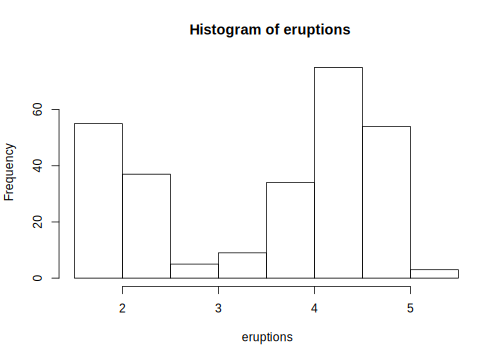
\includegraphics{Rprogramming_files/figure-latex/unnamed-chunk-22-1.pdf}

\begin{Shaded}
\begin{Highlighting}[]
\KeywordTok{hist}\NormalTok{(eruptions, }\KeywordTok{seq}\NormalTok{(}\FloatTok{1.6}\NormalTok{, }\FloatTok{5.2}\NormalTok{, }\FloatTok{0.2}\NormalTok{), }\DataTypeTok{prob=}\OtherTok{TRUE}\NormalTok{)}
\KeywordTok{lines}\NormalTok{(}\KeywordTok{density}\NormalTok{(eruptions, }\DataTypeTok{bw=}\FloatTok{0.1}\NormalTok{))}
\KeywordTok{rug}\NormalTok{(eruptions)}
\NormalTok{?hist}
\NormalTok{?density}
\KeywordTok{lines}\NormalTok{(}\KeywordTok{density}\NormalTok{(eruptions, }\DataTypeTok{bw=}\StringTok{"SJ"}\NormalTok{))}
\end{Highlighting}
\end{Shaded}

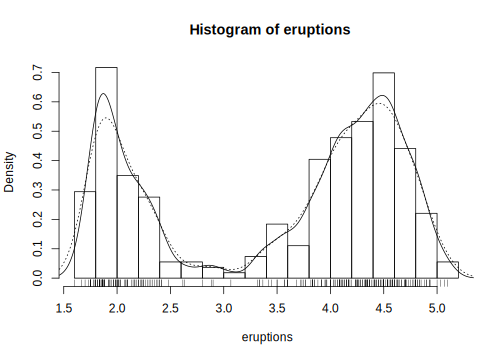
\includegraphics{Rprogramming_files/figure-latex/unnamed-chunk-22-2.pdf}

\begin{Shaded}
\begin{Highlighting}[]
\KeywordTok{plot}\NormalTok{(}\KeywordTok{ecdf}\NormalTok{(eruptions), }\DataTypeTok{do.points=}\OtherTok{FALSE}\NormalTok{, }\DataTypeTok{verticals=}\OtherTok{TRUE}\NormalTok{)}
\end{Highlighting}
\end{Shaded}

\includegraphics{Rprogramming_files/figure-latex/unnamed-chunk-22-3.pdf}

\begin{Shaded}
\begin{Highlighting}[]
\NormalTok{?plot}
\KeywordTok{ecdf}\NormalTok{(eruptions)}
\end{Highlighting}
\end{Shaded}

\begin{verbatim}
## Empirical CDF 
## Call: ecdf(eruptions)
##  x[1:126] = 1.6, 1.7, 1.7,  ..., 5.1, 5.1
\end{verbatim}

\begin{Shaded}
\begin{Highlighting}[]
\NormalTok{x =}\StringTok{ }\KeywordTok{ecdf}\NormalTok{(eruptions)}
\NormalTok{x}
\end{Highlighting}
\end{Shaded}

\begin{verbatim}
## Empirical CDF 
## Call: ecdf(eruptions)
##  x[1:126] = 1.6, 1.7, 1.7,  ..., 5.1, 5.1
\end{verbatim}

\begin{Shaded}
\begin{Highlighting}[]
\KeywordTok{str}\NormalTok{(x)}
\end{Highlighting}
\end{Shaded}

\begin{verbatim}
## function (v)  
##  - attr(*, "class")= chr [1:3] "ecdf" "stepfun" "function"
##  - attr(*, "call")= language ecdf(eruptions)
\end{verbatim}

\begin{Shaded}
\begin{Highlighting}[]
\KeywordTok{x}\NormalTok{()}
\end{Highlighting}
\end{Shaded}

\begin{verbatim}
## Error in .approxfun(x, y, v, method, yleft, yright, f): 기본값이 없는 인수 "v"가 누락되어 있습니다
\end{verbatim}

\begin{Shaded}
\begin{Highlighting}[]
\KeywordTok{plot}\NormalTok{(}\KeywordTok{ecdf}\NormalTok{(eruptions), }\DataTypeTok{do.points=}\OtherTok{FALSE}\NormalTok{)}
\end{Highlighting}
\end{Shaded}

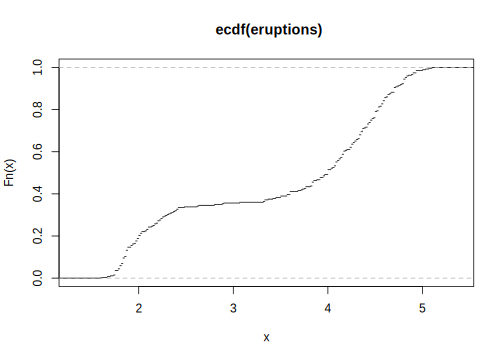
\includegraphics{Rprogramming_files/figure-latex/unnamed-chunk-22-4.pdf}

\begin{Shaded}
\begin{Highlighting}[]
\KeywordTok{plot}\NormalTok{(}\KeywordTok{ecdf}\NormalTok{(eruptions))}
\end{Highlighting}
\end{Shaded}

\includegraphics{Rprogramming_files/figure-latex/unnamed-chunk-22-5.pdf}

\begin{Shaded}
\begin{Highlighting}[]
\NormalTok{long <-}\StringTok{ }\NormalTok{eruptions[eruptions }\OperatorTok{>}\StringTok{ }\DecValTok{3}\NormalTok{]}
\NormalTok{x <-}\StringTok{ }\KeywordTok{seq}\NormalTok{(}\DecValTok{3}\NormalTok{, }\FloatTok{5.4}\NormalTok{, }\FloatTok{0.01}\NormalTok{)}
\KeywordTok{pnorm}\NormalTok{(x, }\DataTypeTok{mean=}\KeywordTok{mean}\NormalTok{(long), }\DataTypeTok{sd=}\KeywordTok{sqrt}\NormalTok{(}\KeywordTok{var}\NormalTok{(long)))}
\end{Highlighting}
\end{Shaded}

\begin{verbatim}
##   [1] 0.0008362 0.0009084 0.0009864 0.0010704 0.0011610
##   [6] 0.0012585 0.0013635 0.0014764 0.0015978 0.0017282
##  [11] 0.0018682 0.0020185 0.0021797 0.0023524 0.0025375
##  [16] 0.0027356 0.0029476 0.0031743 0.0034165 0.0036752
##  [21] 0.0039514 0.0042460 0.0045601 0.0048947 0.0052511
##  [26] 0.0056304 0.0060338 0.0064627 0.0069183 0.0074020
##  [31] 0.0079152 0.0084596 0.0090365 0.0096475 0.0102944
##  [36] 0.0109788 0.0117024 0.0124670 0.0132746 0.0141269
##  [41] 0.0150260 0.0159739 0.0169725 0.0180241 0.0191306
##  [46] 0.0202945 0.0215177 0.0228028 0.0241519 0.0255674
##  [51] 0.0270518 0.0286074 0.0302366 0.0319421 0.0337262
##  [56] 0.0355915 0.0375406 0.0395759 0.0417001 0.0439157
##  [61] 0.0462253 0.0486315 0.0511367 0.0537436 0.0564547
##  [66] 0.0592723 0.0621991 0.0652374 0.0683897 0.0716581
##  [71] 0.0750451 0.0785529 0.0821835 0.0859391 0.0898217
##  [76] 0.0938331 0.0979753 0.1022500 0.1066587 0.1112030
##  [81] 0.1158842 0.1207037 0.1256626 0.1307619 0.1360025
##  [86] 0.1413850 0.1469102 0.1525783 0.1583896 0.1643443
##  [91] 0.1704423 0.1766832 0.1830667 0.1895922 0.1962589
##  [96] 0.2030658 0.2100116 0.2170952 0.2243149 0.2316689
## [101] 0.2391554 0.2467722 0.2545170 0.2623872 0.2703803
## [106] 0.2784932 0.2867229 0.2950662 0.3035195 0.3120794
## [111] 0.3207419 0.3295032 0.3383590 0.3473052 0.3563373
## [116] 0.3654507 0.3746407 0.3839025 0.3932310 0.4026213
## [121] 0.4120681 0.4215661 0.4311100 0.4406943 0.4503134
## [126] 0.4599618 0.4696339 0.4793239 0.4890262 0.4987349
## [131] 0.5084444 0.5181489 0.5278427 0.5375199 0.5471751
## [136] 0.5568024 0.5663963 0.5759512 0.5854617 0.5949224
## [141] 0.6043279 0.6136730 0.6229527 0.6321619 0.6412957
## [146] 0.6503494 0.6593184 0.6681982 0.6769845 0.6856732
## [151] 0.6942601 0.7027416 0.7111139 0.7193735 0.7275172
## [156] 0.7355417 0.7434443 0.7512220 0.7588724 0.7663930
## [161] 0.7737818 0.7810366 0.7881558 0.7951377 0.8019809
## [166] 0.8086842 0.8152465 0.8216671 0.8279453 0.8340805
## [171] 0.8400726 0.8459213 0.8516267 0.8571890 0.8626087
## [176] 0.8678862 0.8730222 0.8780176 0.8828733 0.8875905
## [181] 0.8921703 0.8966142 0.9009236 0.9051002 0.9091456
## [186] 0.9130615 0.9168500 0.9205130 0.9240526 0.9274708
## [191] 0.9307700 0.9339522 0.9370200 0.9399756 0.9428215
## [196] 0.9455601 0.9481939 0.9507254 0.9531571 0.9554916
## [201] 0.9577315 0.9598792 0.9619375 0.9639088 0.9657957
## [206] 0.9676007 0.9693264 0.9709753 0.9725498 0.9740525
## [211] 0.9754857 0.9768519 0.9781534 0.9793926 0.9805717
## [216] 0.9816930 0.9827587 0.9837709 0.9847318 0.9856434
## [221] 0.9865077 0.9873267 0.9881024 0.9888365 0.9895310
## [226] 0.9901874 0.9908077 0.9913933 0.9919460 0.9924672
## [231] 0.9929585 0.9934212 0.9938569 0.9942668 0.9946523
## [236] 0.9950145 0.9953548 0.9956741 0.9959737 0.9962546
## [241] 0.9965177
\end{verbatim}

\begin{Shaded}
\begin{Highlighting}[]
\NormalTok{?par}
\NormalTok{x <-}\StringTok{ }\KeywordTok{rt}\NormalTok{(}\DecValTok{250}\NormalTok{, }\DataTypeTok{df =} \DecValTok{5}\NormalTok{)}
\KeywordTok{qqnorm}\NormalTok{(x); }\KeywordTok{qqline}\NormalTok{(x)}
\end{Highlighting}
\end{Shaded}

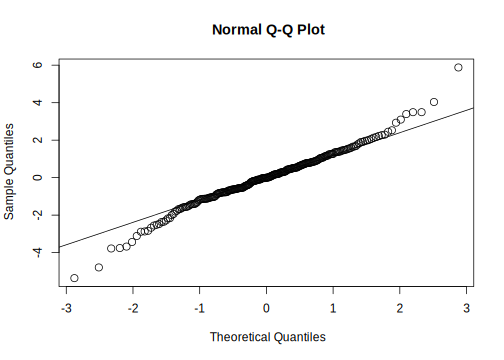
\includegraphics{Rprogramming_files/figure-latex/unnamed-chunk-22-6.pdf}

\begin{Shaded}
\begin{Highlighting}[]
\KeywordTok{curve}\NormalTok{(dnorm, }\OperatorTok{-}\DecValTok{5}\NormalTok{, }\DecValTok{5}\NormalTok{)}
\NormalTok{y =}\StringTok{ }\KeywordTok{density}\NormalTok{(x)}
\KeywordTok{lines}\NormalTok{(y, }\DataTypeTok{lty=}\DecValTok{3}\NormalTok{)}
\end{Highlighting}
\end{Shaded}

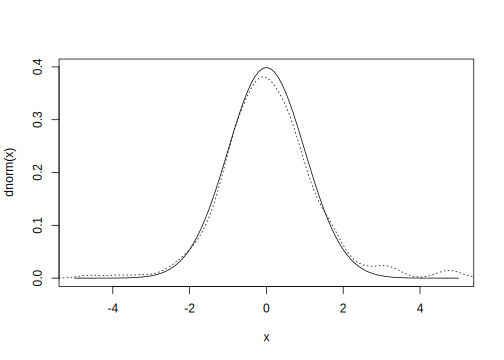
\includegraphics{Rprogramming_files/figure-latex/unnamed-chunk-22-7.pdf}

\begin{Shaded}
\begin{Highlighting}[]
\NormalTok{?ppoints}
\KeywordTok{ppoints}\NormalTok{(}\DecValTok{250}\NormalTok{)}
\end{Highlighting}
\end{Shaded}

\begin{verbatim}
##   [1] 0.002 0.006 0.010 0.014 0.018 0.022 0.026 0.030
##   [9] 0.034 0.038 0.042 0.046 0.050 0.054 0.058 0.062
##  [17] 0.066 0.070 0.074 0.078 0.082 0.086 0.090 0.094
##  [25] 0.098 0.102 0.106 0.110 0.114 0.118 0.122 0.126
##  [33] 0.130 0.134 0.138 0.142 0.146 0.150 0.154 0.158
##  [41] 0.162 0.166 0.170 0.174 0.178 0.182 0.186 0.190
##  [49] 0.194 0.198 0.202 0.206 0.210 0.214 0.218 0.222
##  [57] 0.226 0.230 0.234 0.238 0.242 0.246 0.250 0.254
##  [65] 0.258 0.262 0.266 0.270 0.274 0.278 0.282 0.286
##  [73] 0.290 0.294 0.298 0.302 0.306 0.310 0.314 0.318
##  [81] 0.322 0.326 0.330 0.334 0.338 0.342 0.346 0.350
##  [89] 0.354 0.358 0.362 0.366 0.370 0.374 0.378 0.382
##  [97] 0.386 0.390 0.394 0.398 0.402 0.406 0.410 0.414
## [105] 0.418 0.422 0.426 0.430 0.434 0.438 0.442 0.446
## [113] 0.450 0.454 0.458 0.462 0.466 0.470 0.474 0.478
## [121] 0.482 0.486 0.490 0.494 0.498 0.502 0.506 0.510
## [129] 0.514 0.518 0.522 0.526 0.530 0.534 0.538 0.542
## [137] 0.546 0.550 0.554 0.558 0.562 0.566 0.570 0.574
## [145] 0.578 0.582 0.586 0.590 0.594 0.598 0.602 0.606
## [153] 0.610 0.614 0.618 0.622 0.626 0.630 0.634 0.638
## [161] 0.642 0.646 0.650 0.654 0.658 0.662 0.666 0.670
## [169] 0.674 0.678 0.682 0.686 0.690 0.694 0.698 0.702
## [177] 0.706 0.710 0.714 0.718 0.722 0.726 0.730 0.734
## [185] 0.738 0.742 0.746 0.750 0.754 0.758 0.762 0.766
## [193] 0.770 0.774 0.778 0.782 0.786 0.790 0.794 0.798
## [201] 0.802 0.806 0.810 0.814 0.818 0.822 0.826 0.830
## [209] 0.834 0.838 0.842 0.846 0.850 0.854 0.858 0.862
## [217] 0.866 0.870 0.874 0.878 0.882 0.886 0.890 0.894
## [225] 0.898 0.902 0.906 0.910 0.914 0.918 0.922 0.926
## [233] 0.930 0.934 0.938 0.942 0.946 0.950 0.954 0.958
## [241] 0.962 0.966 0.970 0.974 0.978 0.982 0.986 0.990
## [249] 0.994 0.998
\end{verbatim}

\begin{Shaded}
\begin{Highlighting}[]
\KeywordTok{ppoints}\NormalTok{(}\DecValTok{10}\NormalTok{)}
\end{Highlighting}
\end{Shaded}

\begin{verbatim}
##  [1] 0.06098 0.15854 0.25610 0.35366 0.45122 0.54878
##  [7] 0.64634 0.74390 0.84146 0.93902
\end{verbatim}

\begin{Shaded}
\begin{Highlighting}[]
\KeywordTok{qqplot}\NormalTok{(}\KeywordTok{qt}\NormalTok{(}\KeywordTok{ppoints}\NormalTok{(}\DecValTok{250}\NormalTok{), }\DataTypeTok{df =} \DecValTok{5}\NormalTok{), x, }\DataTypeTok{xlab =} \StringTok{"Q-Q plot for t dsn"}\NormalTok{)}
\end{Highlighting}
\end{Shaded}

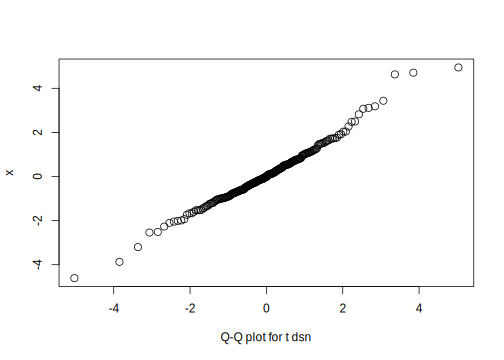
\includegraphics{Rprogramming_files/figure-latex/unnamed-chunk-22-8.pdf}

\begin{Shaded}
\begin{Highlighting}[]
\KeywordTok{windows}\NormalTok{()}
\end{Highlighting}
\end{Shaded}

\begin{verbatim}
## Error in eval(expr, envir, enclos): 함수 "windows"를 찾을 수 없습니다
\end{verbatim}

\begin{Shaded}
\begin{Highlighting}[]
\KeywordTok{qqplot}\NormalTok{(}\KeywordTok{qt}\NormalTok{(}\KeywordTok{runif}\NormalTok{(}\DecValTok{250}\NormalTok{), }\DataTypeTok{df =} \DecValTok{5}\NormalTok{), x, }\DataTypeTok{xlab =} \StringTok{"Q-Q plot for t dsn"}\NormalTok{)}
\end{Highlighting}
\end{Shaded}

\includegraphics{Rprogramming_files/figure-latex/unnamed-chunk-22-9.pdf}

\begin{Shaded}
\begin{Highlighting}[]
\NormalTok{?shapiro.test}
\NormalTok{?ks.test}
\NormalTok{?t.test}


\NormalTok{A =}\StringTok{ }\KeywordTok{c}\NormalTok{(}\FloatTok{79.98}\NormalTok{, }\FloatTok{80.04}\NormalTok{, }\FloatTok{80.02}\NormalTok{, }\FloatTok{80.04}\NormalTok{, }\FloatTok{80.03}\NormalTok{, }\FloatTok{80.03}\NormalTok{, }\FloatTok{80.04}\NormalTok{, }\FloatTok{79.97}\NormalTok{, }\FloatTok{80.05}\NormalTok{, }\FloatTok{80.03}\NormalTok{, }\FloatTok{80.02}\NormalTok{, }\FloatTok{80.00}\NormalTok{, }\FloatTok{80.02}\NormalTok{)}
\NormalTok{B =}\StringTok{ }\KeywordTok{c}\NormalTok{(}\FloatTok{80.02}\NormalTok{, }\FloatTok{79.94}\NormalTok{, }\FloatTok{79.98}\NormalTok{, }\FloatTok{79.97}\NormalTok{, }\FloatTok{79.97}\NormalTok{, }\FloatTok{80.03}\NormalTok{, }\FloatTok{79.95}\NormalTok{, }\FloatTok{79.97}\NormalTok{)}
\KeywordTok{boxplot}\NormalTok{(A, B)}
\end{Highlighting}
\end{Shaded}

\includegraphics{Rprogramming_files/figure-latex/unnamed-chunk-22-10.pdf}

\begin{Shaded}
\begin{Highlighting}[]
\KeywordTok{t.test}\NormalTok{(A, B)}
\end{Highlighting}
\end{Shaded}

\begin{verbatim}
## 
##  Welch Two Sample t-test
## 
## data:  A and B
## t = 3.2, df = 12, p-value = 0.007
## alternative hypothesis: true difference in means is not equal to 0
## 95 percent confidence interval:
##  0.01386 0.07018
## sample estimates:
## mean of x mean of y 
##     80.02     79.98
\end{verbatim}

\begin{Shaded}
\begin{Highlighting}[]
\KeywordTok{var.test}\NormalTok{(A, B)}
\end{Highlighting}
\end{Shaded}

\begin{verbatim}
## 
##  F test to compare two variances
## 
## data:  A and B
## F = 0.58, num df = 12, denom df = 7, p-value =
## 0.4
## alternative hypothesis: true ratio of variances is not equal to 1
## 95 percent confidence interval:
##  0.1251 2.1053
## sample estimates:
## ratio of variances 
##             0.5837
\end{verbatim}

\begin{Shaded}
\begin{Highlighting}[]
\KeywordTok{t.test}\NormalTok{(A, B, }\DataTypeTok{var.equal=}\OtherTok{TRUE}\NormalTok{)}
\end{Highlighting}
\end{Shaded}

\begin{verbatim}
## 
##  Two Sample t-test
## 
## data:  A and B
## t = 3.5, df = 19, p-value = 0.003
## alternative hypothesis: true difference in means is not equal to 0
## 95 percent confidence interval:
##  0.01669 0.06735
## sample estimates:
## mean of x mean of y 
##     80.02     79.98
\end{verbatim}

\begin{Shaded}
\begin{Highlighting}[]
\KeywordTok{wilcox.test}\NormalTok{(A, B)}
\end{Highlighting}
\end{Shaded}

\begin{verbatim}
## Warning in wilcox.test.default(A, B): cannot compute
## exact p-value with ties
\end{verbatim}

\begin{verbatim}
## 
##  Wilcoxon rank sum test with continuity
##  correction
## 
## data:  A and B
## W = 89, p-value = 0.007
## alternative hypothesis: true location shift is not equal to 0
\end{verbatim}

\begin{Shaded}
\begin{Highlighting}[]
\KeywordTok{plot}\NormalTok{(}\KeywordTok{ecdf}\NormalTok{(A), }\DataTypeTok{do.points=}\OtherTok{FALSE}\NormalTok{, }\DataTypeTok{verticals=}\OtherTok{TRUE}\NormalTok{, }\DataTypeTok{xlim=}\KeywordTok{range}\NormalTok{(A, B))}
\KeywordTok{plot}\NormalTok{(}\KeywordTok{ecdf}\NormalTok{(B), }\DataTypeTok{do.points=}\OtherTok{FALSE}\NormalTok{, }\DataTypeTok{verticals=}\OtherTok{TRUE}\NormalTok{, }\DataTypeTok{add=}\OtherTok{TRUE}\NormalTok{)}
\end{Highlighting}
\end{Shaded}

\includegraphics{Rprogramming_files/figure-latex/unnamed-chunk-22-11.pdf}

\begin{Shaded}
\begin{Highlighting}[]
\KeywordTok{ks.test}\NormalTok{(A, B)}
\end{Highlighting}
\end{Shaded}

\begin{verbatim}
## Warning in ks.test(A, B): cannot compute exact p-value
## with ties
\end{verbatim}

\begin{verbatim}
## 
##  Two-sample Kolmogorov-Smirnov test
## 
## data:  A and B
## D = 0.6, p-value = 0.06
## alternative hypothesis: two-sided
\end{verbatim}

\begin{Shaded}
\begin{Highlighting}[]
\CommentTok{# Chapter 9 Grouping, loops and conditional execution}

\CommentTok{# \{ \} does grouping}
\CommentTok{# Usefulness of loops: for >> while >> repeat}
\ControlFlowTok{for}\NormalTok{ (i }\ControlFlowTok{in} \DecValTok{1}\OperatorTok{:}\DecValTok{10}\NormalTok{) \{}
  \KeywordTok{print}\NormalTok{(}\DecValTok{2}\OperatorTok{*}\NormalTok{i)}
\NormalTok{\}}
\end{Highlighting}
\end{Shaded}

\begin{verbatim}
## [1] 2
## [1] 4
## [1] 6
## [1] 8
## [1] 10
## [1] 12
## [1] 14
## [1] 16
## [1] 18
## [1] 20
\end{verbatim}

\begin{Shaded}
\begin{Highlighting}[]
\CommentTok{# # if ~ else ~}
\CommentTok{# if (   ) \{}
\CommentTok{# # Statements 1}
\CommentTok{# \} else \{}
\CommentTok{# # Statements 2}
\CommentTok{# \}}
\CommentTok{# }
\CommentTok{# if (   ) \{}
\CommentTok{# # Statements 1}
\CommentTok{# \} else if (   ) \{}
\CommentTok{# # Statements 2}
\CommentTok{# \} else if (   ) \{}
\CommentTok{# # Statements 3}
\CommentTok{# \} else \{}
\CommentTok{# # Statements 4  }
\CommentTok{# \}}

   
\CommentTok{#}
\CommentTok{#}

\CommentTok{# Chapter 10 Writing your own functions}

\NormalTok{twosam =}\StringTok{ }\ControlFlowTok{function}\NormalTok{(y1, y2) }
\NormalTok{\{}
\NormalTok{  n1  =}\StringTok{ }\KeywordTok{length}\NormalTok{(y1)}
\NormalTok{  n2  =}\StringTok{ }\KeywordTok{length}\NormalTok{(y2)}
\NormalTok{  yb1 =}\StringTok{ }\KeywordTok{mean}\NormalTok{(y1)}
\NormalTok{  yb2 =}\StringTok{ }\KeywordTok{mean}\NormalTok{(y2)}
\NormalTok{  s1  =}\StringTok{ }\KeywordTok{var}\NormalTok{(y1)}
\NormalTok{  s2  =}\StringTok{ }\KeywordTok{var}\NormalTok{(y2) }
\NormalTok{  s   =}\StringTok{ }\NormalTok{((n1 }\OperatorTok{-}\StringTok{ }\DecValTok{1}\NormalTok{)}\OperatorTok{*}\NormalTok{s1 }\OperatorTok{+}\StringTok{ }\NormalTok{(n2 }\OperatorTok{-}\StringTok{ }\DecValTok{1}\NormalTok{)}\OperatorTok{*}\NormalTok{s2)}\OperatorTok{/}\NormalTok{(n1 }\OperatorTok{+}\StringTok{ }\NormalTok{n2 }\OperatorTok{-}\StringTok{ }\DecValTok{2}\NormalTok{)}
\NormalTok{  tst =}\StringTok{ }\NormalTok{(yb1 }\OperatorTok{-}\StringTok{ }\NormalTok{yb2)}\OperatorTok{/}\KeywordTok{sqrt}\NormalTok{(s}\OperatorTok{*}\NormalTok{(}\DecValTok{1}\OperatorTok{/}\NormalTok{n1 }\OperatorTok{+}\StringTok{ }\DecValTok{1}\OperatorTok{/}\NormalTok{n2))}
  \KeywordTok{return}\NormalTok{ (tst)}
\NormalTok{\}}

\NormalTok{x =}\StringTok{ }\KeywordTok{rnorm}\NormalTok{(}\DecValTok{10}\NormalTok{)}
\NormalTok{y =}\StringTok{ }\KeywordTok{rt}\NormalTok{(}\DecValTok{10}\NormalTok{, }\DecValTok{5}\NormalTok{)}

\KeywordTok{twosam}\NormalTok{(x, y)}
\end{Highlighting}
\end{Shaded}

\begin{verbatim}
## [1] 1.708
\end{verbatim}

\begin{Shaded}
\begin{Highlighting}[]
\NormalTok{T.test =}\StringTok{ }\ControlFlowTok{function}\NormalTok{(y1, y2) }
\NormalTok{\{}
\NormalTok{  n1  =}\StringTok{ }\KeywordTok{length}\NormalTok{(y1)}
\NormalTok{  n2  =}\StringTok{ }\KeywordTok{length}\NormalTok{(y2)}
\NormalTok{  yb1 =}\StringTok{ }\KeywordTok{mean}\NormalTok{(y1)}
\NormalTok{  yb2 =}\StringTok{ }\KeywordTok{mean}\NormalTok{(y2)}
\NormalTok{  s1  =}\StringTok{ }\KeywordTok{var}\NormalTok{(y1)}
\NormalTok{  s2  =}\StringTok{ }\KeywordTok{var}\NormalTok{(y2) }
\NormalTok{  s   =}\StringTok{ }\NormalTok{((n1 }\OperatorTok{-}\StringTok{ }\DecValTok{1}\NormalTok{)}\OperatorTok{*}\NormalTok{s1 }\OperatorTok{+}\StringTok{ }\NormalTok{(n2 }\OperatorTok{-}\StringTok{ }\DecValTok{1}\NormalTok{)}\OperatorTok{*}\NormalTok{s2)}\OperatorTok{/}\NormalTok{(n1 }\OperatorTok{+}\StringTok{ }\NormalTok{n2 }\OperatorTok{-}\StringTok{ }\DecValTok{2}\NormalTok{)}

\NormalTok{  tst =}\StringTok{ }\NormalTok{(yb1 }\OperatorTok{-}\StringTok{ }\NormalTok{yb2)}\OperatorTok{/}\KeywordTok{sqrt}\NormalTok{(s}\OperatorTok{*}\NormalTok{(}\DecValTok{1}\OperatorTok{/}\NormalTok{n1 }\OperatorTok{+}\StringTok{ }\DecValTok{1}\OperatorTok{/}\NormalTok{n2))}
\NormalTok{  DF =}\StringTok{ }\NormalTok{n1 }\OperatorTok{+}\StringTok{ }\NormalTok{n2 }\OperatorTok{-}\StringTok{ }\DecValTok{2}
\NormalTok{  p.val =}\StringTok{ }\KeywordTok{pt}\NormalTok{(tst, }\DataTypeTok{df=}\NormalTok{DF)}
  
\NormalTok{  Res =}\StringTok{ }\KeywordTok{list}\NormalTok{(tst, DF, p.val)}
  \KeywordTok{names}\NormalTok{(Res) =}\StringTok{ }\KeywordTok{c}\NormalTok{(}\StringTok{"t"}\NormalTok{, }\StringTok{"df"}\NormalTok{, }\StringTok{"p-value"}\NormalTok{)}
  
  \KeywordTok{return}\NormalTok{ (Res)}
\NormalTok{\}}

\KeywordTok{T.test}\NormalTok{(x, y)}
\end{Highlighting}
\end{Shaded}

\begin{verbatim}
## $t
## [1] 1.708
## 
## $df
## [1] 18
## 
## $`p-value`
## [1] 0.9475
\end{verbatim}

\begin{Shaded}
\begin{Highlighting}[]
\NormalTok{bslash =}\StringTok{ }\ControlFlowTok{function}\NormalTok{(X, y) }
\NormalTok{\{}
\NormalTok{  X =}\StringTok{ }\KeywordTok{qr}\NormalTok{(X)}
  \KeywordTok{return}\NormalTok{ (}\KeywordTok{qr.coef}\NormalTok{(X, y))}
\NormalTok{\}}

\NormalTok{regcoeff =}\StringTok{ }\KeywordTok{bslash}\NormalTok{(Xmat, yvar)}
\end{Highlighting}
\end{Shaded}

\begin{verbatim}
## Error in qr(X): 객체 'Xmat'를 찾을 수 없습니다
\end{verbatim}

\begin{Shaded}
\begin{Highlighting}[]
\StringTok{"%^%"}\NormalTok{ =}\StringTok{ }\ControlFlowTok{function}\NormalTok{(S, pow) }\KeywordTok{with}\NormalTok{(}\KeywordTok{eigen}\NormalTok{(S), vectors }\OperatorTok\StringTok{ }\NormalTok{(}\KeywordTok{abs}\NormalTok{(values)}\OperatorTok{^}\NormalTok{pow }\OperatorTok{*}\StringTok{ }\KeywordTok{t}\NormalTok{(vectors)))}

\NormalTok{M =}\StringTok{ }\KeywordTok{matrix}\NormalTok{(}\KeywordTok{c}\NormalTok{(}\DecValTok{2}\NormalTok{,}\DecValTok{1}\NormalTok{,}\DecValTok{1}\NormalTok{,}\DecValTok{2}\NormalTok{), }\DataTypeTok{nrow=}\DecValTok{2}\NormalTok{) ; M}
\end{Highlighting}
\end{Shaded}

\begin{verbatim}
##      [,1] [,2]
## [1,]    2    1
## [2,]    1    2
\end{verbatim}

\begin{Shaded}
\begin{Highlighting}[]
\NormalTok{M }\OperatorTok\StringTok{ }\FloatTok{0.5}
\end{Highlighting}
\end{Shaded}

\begin{verbatim}
##       [,1]  [,2]
## [1,] 1.366 0.366
## [2,] 0.366 1.366
\end{verbatim}

\begin{Shaded}
\begin{Highlighting}[]
\NormalTok{sqrtM =}\StringTok{ }\NormalTok{M}\OperatorTok\FloatTok{0.5}\NormalTok{ ; sqrtM}
\end{Highlighting}
\end{Shaded}

\begin{verbatim}
##       [,1]  [,2]
## [1,] 1.366 0.366
## [2,] 0.366 1.366
\end{verbatim}

\begin{Shaded}
\begin{Highlighting}[]
\NormalTok{sqrtM }\OperatorTok\StringTok{ }\NormalTok{sqrtM}
\end{Highlighting}
\end{Shaded}

\begin{verbatim}
##      [,1] [,2]
## [1,]    2    1
## [2,]    1    2
\end{verbatim}

\begin{Shaded}
\begin{Highlighting}[]
\NormalTok{area =}\StringTok{ }\ControlFlowTok{function}\NormalTok{(f, a, b, }\DataTypeTok{eps=}\FloatTok{1.0e-06}\NormalTok{, }\DataTypeTok{lim=}\DecValTok{10}\NormalTok{) }
\NormalTok{\{}
\NormalTok{  fun1 =}\StringTok{ }\ControlFlowTok{function}\NormalTok{(f, a, b, fa, fb, a0, eps, lim, fun) }
\NormalTok{  \{}
\NormalTok{  ## function 'fun1'is only visible inside 'area'}
\NormalTok{    d =}\StringTok{ }\NormalTok{(a }\OperatorTok{+}\StringTok{ }\NormalTok{b)}\OperatorTok{/}\DecValTok{2}
\NormalTok{    h =}\StringTok{ }\NormalTok{(b }\OperatorTok{-}\StringTok{ }\NormalTok{a)}\OperatorTok{/}\DecValTok{4}
\NormalTok{    fd =}\StringTok{ }\KeywordTok{f}\NormalTok{(d)}
\NormalTok{    a1 =}\StringTok{ }\NormalTok{h }\OperatorTok{*}\StringTok{ }\NormalTok{(fa }\OperatorTok{+}\StringTok{ }\NormalTok{fd)}
\NormalTok{    a2 =}\StringTok{ }\NormalTok{h }\OperatorTok{*}\StringTok{ }\NormalTok{(fd }\OperatorTok{+}\StringTok{ }\NormalTok{fb)}
    \ControlFlowTok{if}\NormalTok{ (}\KeywordTok{abs}\NormalTok{(a0 }\OperatorTok{-}\StringTok{ }\NormalTok{a1 }\OperatorTok{-}\StringTok{ }\NormalTok{a2) }\OperatorTok{<}\StringTok{ }\NormalTok{eps }\OperatorTok{||}\StringTok{ }\NormalTok{lim }\OperatorTok{==}\StringTok{ }\DecValTok{0}\NormalTok{)}
      \KeywordTok{return}\NormalTok{ (a1 }\OperatorTok{+}\StringTok{ }\NormalTok{a2)}
    \ControlFlowTok{else}\NormalTok{ \{}
      \KeywordTok{return}\NormalTok{ (}\KeywordTok{fun}\NormalTok{(f, a, d, fa, fd, a1, eps, lim }\OperatorTok{-}\StringTok{ }\DecValTok{1}\NormalTok{, fun) }\OperatorTok{+}\StringTok{ }\KeywordTok{fun}\NormalTok{(f, d, b, fd, fb, a2, eps, lim }\OperatorTok{-}\StringTok{ }\DecValTok{1}\NormalTok{, fun))}
\NormalTok{    \}}
\NormalTok{  \}}
\NormalTok{  fa =}\StringTok{ }\KeywordTok{f}\NormalTok{(a)}
\NormalTok{  fb =}\StringTok{ }\KeywordTok{f}\NormalTok{(b)}
\NormalTok{  a0 =}\StringTok{ }\NormalTok{((fa }\OperatorTok{+}\StringTok{ }\NormalTok{fb) }\OperatorTok{*}\StringTok{ }\NormalTok{(b }\OperatorTok{-}\StringTok{ }\NormalTok{a))}\OperatorTok{/}\DecValTok{2}
  \KeywordTok{fun1}\NormalTok{(f, a, b, fa, fb, a0, eps, lim, fun1)}
\NormalTok{\} }

\KeywordTok{area}\NormalTok{(dnorm, }\DecValTok{0}\NormalTok{, }\DecValTok{1}\NormalTok{)}
\end{Highlighting}
\end{Shaded}

\begin{verbatim}
## [1] 0.3413
\end{verbatim}

\begin{Shaded}
\begin{Highlighting}[]
\KeywordTok{integrate}\NormalTok{(dnorm, }\DecValTok{0}\NormalTok{, }\DecValTok{1}\NormalTok{)}
\end{Highlighting}
\end{Shaded}

\begin{verbatim}
## 0.3413 with absolute error < 3.8e-15
\end{verbatim}

\begin{Shaded}
\begin{Highlighting}[]
\KeywordTok{pnorm}\NormalTok{(}\DecValTok{1}\NormalTok{) }\OperatorTok{-}\StringTok{ }\KeywordTok{pnorm}\NormalTok{(}\DecValTok{0}\NormalTok{)}
\end{Highlighting}
\end{Shaded}

\begin{verbatim}
## [1] 0.3413
\end{verbatim}

\begin{Shaded}
\begin{Highlighting}[]
\NormalTok{f =}\StringTok{ }\ControlFlowTok{function}\NormalTok{(x) }
\NormalTok{\{}
\NormalTok{  y =}\StringTok{ }\DecValTok{2}\OperatorTok{*}\NormalTok{x}
  \KeywordTok{print}\NormalTok{(x)}
  \KeywordTok{print}\NormalTok{(y)}
  \KeywordTok{print}\NormalTok{(z)}
\NormalTok{\}}

\KeywordTok{f}\NormalTok{(}\DecValTok{1}\NormalTok{)}
\end{Highlighting}
\end{Shaded}

\begin{verbatim}
## [1] 1
## [1] 2
\end{verbatim}

\begin{verbatim}
## Error in print(z): 객체 'z'를 찾을 수 없습니다
\end{verbatim}

\begin{Shaded}
\begin{Highlighting}[]
\NormalTok{z =}\StringTok{ }\DecValTok{3}
\KeywordTok{f}\NormalTok{(}\DecValTok{1}\NormalTok{)}
\end{Highlighting}
\end{Shaded}

\begin{verbatim}
## [1] 1
## [1] 2
## [1] 3
\end{verbatim}

\begin{Shaded}
\begin{Highlighting}[]
\NormalTok{cube =}\StringTok{ }\ControlFlowTok{function}\NormalTok{(n) \{}
\NormalTok{  sq =}\StringTok{ }\ControlFlowTok{function}\NormalTok{() n}\OperatorTok{*}\NormalTok{n}
\NormalTok{  n}\OperatorTok{*}\KeywordTok{sq}\NormalTok{()}
\NormalTok{\}}

\KeywordTok{cube}\NormalTok{(}\DecValTok{5}\NormalTok{)}
\end{Highlighting}
\end{Shaded}

\begin{verbatim}
## [1] 125
\end{verbatim}

\begin{Shaded}
\begin{Highlighting}[]
\NormalTok{open.account =}\StringTok{ }\ControlFlowTok{function}\NormalTok{(total) }
\NormalTok{\{}
  \KeywordTok{list}\NormalTok{(}
    \DataTypeTok{deposit =} \ControlFlowTok{function}\NormalTok{(amount) }
\NormalTok{    \{}
      \ControlFlowTok{if}\NormalTok{(amount }\OperatorTok{<=}\StringTok{ }\DecValTok{0}\NormalTok{)}
      \KeywordTok{stop}\NormalTok{(}\StringTok{"Deposits must be positive!}\CharTok{\textbackslash{}n}\StringTok{"}\NormalTok{)}
\NormalTok{      total <<-}\StringTok{ }\NormalTok{total }\OperatorTok{+}\StringTok{ }\NormalTok{amount}
      \KeywordTok{cat}\NormalTok{(amount, }\StringTok{"deposited. Your balance is"}\NormalTok{, total, }\StringTok{"}\CharTok{\textbackslash{}n\textbackslash{}n}\StringTok{"}\NormalTok{)}
\NormalTok{    \},}
    \DataTypeTok{withdraw =} \ControlFlowTok{function}\NormalTok{(amount) }
\NormalTok{    \{}
      \ControlFlowTok{if}\NormalTok{(amount }\OperatorTok{>}\StringTok{ }\NormalTok{total)}
      \KeywordTok{stop}\NormalTok{(}\StringTok{"You don't have that much money!}\CharTok{\textbackslash{}n}\StringTok{"}\NormalTok{)}
\NormalTok{      total <<-}\StringTok{ }\NormalTok{total }\OperatorTok{-}\StringTok{ }\NormalTok{amount}
      \KeywordTok{cat}\NormalTok{(amount, }\StringTok{"withdrawn. Your balance is"}\NormalTok{, total, }\StringTok{"}\CharTok{\textbackslash{}n\textbackslash{}n}\StringTok{"}\NormalTok{)}
\NormalTok{    \},}
    \DataTypeTok{balance =} \ControlFlowTok{function}\NormalTok{() }
\NormalTok{    \{}
      \KeywordTok{cat}\NormalTok{(}\StringTok{"Your balance is"}\NormalTok{, total, }\StringTok{"}\CharTok{\textbackslash{}n\textbackslash{}n}\StringTok{"}\NormalTok{)}
\NormalTok{    \}}
\NormalTok{  )}
\NormalTok{\}}

\NormalTok{ross =}\StringTok{ }\KeywordTok{open.account}\NormalTok{(}\DecValTok{100}\NormalTok{)}
\NormalTok{robert =}\StringTok{ }\KeywordTok{open.account}\NormalTok{(}\DecValTok{200}\NormalTok{)}

\NormalTok{ross}\OperatorTok{$}\KeywordTok{balance}\NormalTok{()}
\end{Highlighting}
\end{Shaded}

\begin{verbatim}
## Your balance is 100
\end{verbatim}

\begin{Shaded}
\begin{Highlighting}[]
\NormalTok{robert}\OperatorTok{$}\KeywordTok{balance}\NormalTok{()}
\end{Highlighting}
\end{Shaded}

\begin{verbatim}
## Your balance is 200
\end{verbatim}

\begin{Shaded}
\begin{Highlighting}[]
\NormalTok{ross}\OperatorTok{$}\KeywordTok{deposit}\NormalTok{(}\DecValTok{50}\NormalTok{)}
\end{Highlighting}
\end{Shaded}

\begin{verbatim}
## 50 deposited. Your balance is 150
\end{verbatim}

\begin{Shaded}
\begin{Highlighting}[]
\NormalTok{ross}\OperatorTok{$}\KeywordTok{balance}\NormalTok{()}
\end{Highlighting}
\end{Shaded}

\begin{verbatim}
## Your balance is 150
\end{verbatim}

\begin{Shaded}
\begin{Highlighting}[]
\NormalTok{ross}\OperatorTok{$}\KeywordTok{withdraw}\NormalTok{(}\DecValTok{500}\NormalTok{)}
\end{Highlighting}
\end{Shaded}

\begin{verbatim}
## Error in ross$withdraw(500): You don't have that much money!
\end{verbatim}

\section{The basics}\label{the-basics}

\begin{table}

\caption{\label{tab:knitchunk1}The basics - The first functions to learn}
\centering
\begin{tabular}[t]{llll}
\toprule
Keyword & Bae Freq & Essential & Comment\\
\midrule
? & H & Y & \\
str & M & Y & strucutre\\
\bottomrule
\end{tabular}
\end{table}

\begin{table}

\caption{\label{tab:knitchunk2}The basics - Important operators and assignment}
\centering
\begin{tabular}[t]{llll}
\toprule
Keyword & Bae Freq & Essential & Comment\\
\midrule
\%in\% & M & Y & Value Matching\\
match & M & N & Value Matching\\
= & H & Y & \\
<- & L & N & \\
<<- & M & Y & \\
\addlinespace
head & H & N & \\
tail & M & N & \\
subset & L & N & Subsetting Vectors, Matrices and Data Frames\\
with & L & N & Evaluate an Expression in a Data Environment\\
assign & L & N & Assign a Value to a Name\\
get & L & N & Return the Value of a Named Object\\
\bottomrule
\end{tabular}
\end{table}

\begin{table}

\caption{\label{tab:knitchunk3}The basics - Comparison }
\centering
\begin{tabular}[t]{llll}
\toprule
Keyword & Bae Freq & Essential & Comment\\
\midrule
all.equal & L & N & Test if Two Objects are (Nearly) Equal\\
identical & L & N & Test Objects for Exact Equality\\
!=, ==, >, >=, <, <= & H & Y & Comparison Operator\\
is.na & H & Y & \\
complete.cases & L & N & Find Complete Cases\\
is.finite & M & Y & \\
\bottomrule
\end{tabular}
\end{table}

\begin{table}

\caption{\label{tab:knitchunk4}The basics - Basic math}
\centering
\begin{tabular}[t]{llll}
\toprule
Keyword & Bae Freq & Essential & Comment\\
\midrule
*, +, -, /, \textasciicircum{} & H & Y & Math operator\\
\%\% & M & Y & Modulus\\
\%/\% & L & N & Integer division\\
abs & H & Y & \\
sign & M & N & \\
\addlinespace
acos & L & Y & \\
asin & L & Y & \\
atan & L & Y & \\
atan2 & L & Y & \\
sin & L & Y & \\
\addlinespace
cos & L & Y & \\
tan & L & Y & \\
ceiling & H & Y & \\
floor & H & N & \\
round & H & Y & \\
\addlinespace
trunc & H & N & \\
signif & M & Y & rounds the values in its first argument to the specified number of significant digits\\
exp & H & Y & \\
log & H & Y & \\
log10 & L & Y & \\
\addlinespace
log2 & L & Y & \\
sqrt & H & N & \\
max & H & Y & \\
min & H & Y & \\
prod & L & N & \\
\addlinespace
sum & H & Y & \\
cummax & L & N & \\
cummin & L & N & \\
cumprod & L & N & \\
cumsum & L & N & \\
\addlinespace
diff & L & N & \\
pmax & L & N & pairwise max\\
pmin & L & N & pairwise min\\
range & L & N & \\
mean & H & Y & \\
\addlinespace
median & H & Y & \\
cor & H & Y & \\
sd & H & Y & \\
var & H & Y & \\
rle & L & N & Run Length Encoding\\
\bottomrule
\end{tabular}
\end{table}

\begin{table}

\caption{\label{tab:knitchunk5}The basics - Functions to do with functions}
\centering
\begin{tabular}[t]{llll}
\toprule
Keyword & Bae Freq & Essential & Comment\\
\midrule
function & H & Y & \\
missing & M & Y & Does a Formal Argument have a Value?\\
on.exit & L & Y & \\
return & H & N & \\
invisible & L & N & Change the Print Mode to Invisible\\
\bottomrule
\end{tabular}
\end{table}

\begin{table}

\caption{\label{tab:knitchunk6}The basics - Logical - sets }
\centering
\begin{tabular}[t]{llll}
\toprule
Keyword & Bae Freq & Essential & Comment\\
\midrule
\&, |, ! & H & Y & \\
xor & L & Y & \\
all & L & Y & Are All Values True?\\
any & L & Y & Are Some Values True?\\
intersect & M & Y & \\
\addlinespace
union & M & Y & \\
setdiff & L & Y & \\
setequal & L & Y & \\
which & L & N & Which indices are TRUE?\\
\bottomrule
\end{tabular}
\end{table}

\begin{table}

\caption{\label{tab:knitchunk7}The basics - Vectors and matrices}
\centering
\begin{tabular}[t]{llll}
\toprule
Keyword & Bae Freq & Essential & Comment\\
\midrule
c & H & Y & \\
matrix & H & Y & \\
\# automatic coercion rules character > numeric > logical & H & Y & \\
length & H & Y & \\
dim & H & Y & \\
\addlinespace
ncol & H & N & \\
nrow & H & N & \\
cbind & H & Y & \\
rbind & H & Y & \\
names & M & Y & \\
\addlinespace
colnames & H & Y & \\
rownames & M & Y & \\
t & H & Y & \\
diag & H & Y & \\
sweep & L & N & Sweep out Array Summaries\\
\addlinespace
as.matrix & H & Y & \\
data.matrix & L & N & Convert a Data Frame to a Numeric Matrix\\
\bottomrule
\end{tabular}
\end{table}

\begin{table}

\caption{\label{tab:knitchunk8}The basics - Making vectors }
\centering
\begin{tabular}[t]{llll}
\toprule
Keyword & Bae Freq & Essential & Comment\\
\midrule
c & H & Y & \\
rep & H & Y & \\
rep\_len & L & N & Replicate Elements of Vectors and Lists with length.out\\
seq & M & Y & \\
seq\_len & L & N & \\
\addlinespace
seq\_along & L & N & \\
rev & M & Y & \\
sample & H & Y & \\
choose & H & Y & \\
factorial & M & Y & \\
\addlinespace
combn & L & N & Generate All Combinations of n Elements, Taken m at a Time\\
(is/as).(character/numeric/logical/...) & H & Y & \\
\bottomrule
\end{tabular}
\end{table}

\begin{table}

\caption{\label{tab:knitchunk9}The basics - Lists - data.frames }
\centering
\begin{tabular}[t]{llll}
\toprule
Keyword & Bae Freq & Essential & Comment\\
\midrule
list & H & Y & \\
unlist & L & Y & Flatten Lists\\
data.frame & H & Y & \\
as.data.frame & H & Y & \\
split & H & Y & \\
expand.grid & L & N & Create a Data Frame from All Combinations of Factor Variables\\
\bottomrule
\end{tabular}
\end{table}

\begin{table}

\caption{\label{tab:knitchunk10}The basics - Control flow }
\centering
\begin{tabular}[t]{llll}
\toprule
Keyword & Bae Freq & Essential & Comment\\
\midrule
if & H & Y & \\
\&\& & L & Y & \\
|| (short circuiting) & L & Y & \\
for & H & Y & \\
while & L & N & \\
\addlinespace
next & M & Y & \\
break & M & Y & \\
switch & L & Y & \\
ifelse & L & N & Conditional Element Selection\\
\bottomrule
\end{tabular}
\end{table}

\begin{table}

\caption{\label{tab:knitchunk11}The basics - Apply - friends}
\centering
\begin{tabular}[t]{llll}
\toprule
Keyword & Bae Freq & Essential & Comment\\
\midrule
lapply & L & N & Apply a Function over a List or Vector\\
sapply & L & N & user-friendly version and wrapper of lapply\\
vapply & L & N & similar to sapply, but has a pre-specified type of return value\\
apply & M & N & Apply Functions Over Array Margins\\
tapply & L & N & Apply a Function Over a Ragged Array\\
replicate & L & N & Apply a Function over a List or Vector\\
\bottomrule
\end{tabular}
\end{table}

\section{Common data structures}\label{common-data-structures}

\begin{table}

\caption{\label{tab:knitchunk12}Common data structures - Date time}
\centering
\begin{tabular}[t]{llll}
\toprule
Keyword & Bae Freq & Essential & Comment\\
\midrule
ISOdate & L & N & \\
ISOdatetime & L & N & \\
strftime & H & Y & Date-time Conversion Functions to and from Character\\
strptime & H & Y & Date-time Conversion Functions to and from Character\\
date & M & Y & \\
\addlinespace
difftime & H & Y & \\
julian & L & Y & Extract Parts of a POSIXt or Date Object\\
months & L & N & Extract Parts of a POSIXt or Date Object\\
quarters & L & N & Extract Parts of a POSIXt or Date Object\\
weekdays & L & N & Extract Parts of a POSIXt or Date Object\\
library(lubridate) & L & N & \\
\bottomrule
\end{tabular}
\end{table}

\begin{table}

\caption{\label{tab:knitchunk13}Common data structures - Character manipulation }
\centering
\begin{tabular}[t]{llll}
\toprule
Keyword & Bae Freq & Essential & Comment\\
\midrule
grep & H & Y & Pattern Matching and Replacement\\
agrep & L & N & Approximate String Matching (Fuzzy Matching)\\
gsub & M & Y & or use sub\\
strsplit & H & Y & \\
chartr & L & N & Character Translation and Casefolding\\
\addlinespace
nchar & M & Y & \\
tolower & M & Y & \\
toupper & H & Y & \\
substr & H & Y & \\
paste & H & Y & \\
library(stringr) & L & N & \\
\bottomrule
\end{tabular}
\end{table}

\begin{table}

\caption{\label{tab:knitchunk14}Common data structures - Factors }
\centering
\begin{tabular}[t]{llll}
\toprule
Keyword & Bae Freq & Essential & Comment\\
\midrule
factor & M & Y & \\
levels & M & Y & \\
nlevels & L & N & \\
reorder & L & N & Reorder Levels of a Factor\\
relevel & L & N & Reorder Levels of Factor\\
\addlinespace
cut & L & Y & \\
findInterval & L & N & Find Interval Numbers or Indices\\
interaction & L & N & Compute Factor Interactions\\
options(stringsAsFactors = FALSE) & L & N & \\
\bottomrule
\end{tabular}
\end{table}

\begin{table}

\caption{\label{tab:knitchunk15}Common data structures - Array manipulation}
\centering
\begin{tabular}[t]{llll}
\toprule
Keyword & Bae Freq & Essential & Comment\\
\midrule
array & L & N & Multi-way Arrays\\
dim & H & Y & \\
dimnames & M & Y & \\
aperm & L & N & Array Transposition\\
library(abind) & L & N & \\
\bottomrule
\end{tabular}
\end{table}

\section{Statistics}\label{statistics}

\begin{table}

\caption{\label{tab:knitchunk16}Statistics - Ordering and tabulating }
\centering
\begin{tabular}[t]{llll}
\toprule
Keyword & Bae Freq & Essential & Comment\\
\midrule
duplicated & L & Y & Determine Duplicated Elements\\
unique & H & Y & \\
merge & L & N & \\
order & H & Y & \\
rank & L & Y & \\
\addlinespace
quantile & L & Y & \\
sort & H & Y & \\
table & M & Y & \\
ftable & L & Y & Flat Contingency Tables\\
\bottomrule
\end{tabular}
\end{table}

\begin{table}

\caption{\label{tab:knitchunk17}Statistics - Linear models }
\centering
\begin{tabular}[t]{llll}
\toprule
Keyword & Bae Freq & Essential & Comment\\
\midrule
fitted & L & Y & Extract Model Fitted Values\\
predict & H & Y & \\
resid & L & Y & Extract Model Residuals\\
rstandard & L & Y & Regression Deletion Diagnostics\\
lm & H & Y & \\
\addlinespace
glm & H & Y & \\
hat & L & Y & \\
influence.measures & M & Y & Regression Deletion Diagnostics\\
logLik & L & Y & \\
df & M & Y & \\
\addlinespace
deviance & M & Y & \\
formula & H & Y & \\
\textasciitilde{} & H & Y & \\
I & H & Y & \\
anova & H & Y & \\
\addlinespace
coef & M & Y & \\
confint & M & Y & \\
vcov & H & Y & \\
contrasts & L & Y & Get and Set Contrast Matrices\\
\bottomrule
\end{tabular}
\end{table}

\begin{table}

\caption{\label{tab:knitchunk18}Statistics - Miscellaneous tests}
\centering
\begin{tabular}[t]{llll}
\toprule
Keyword & Bae Freq & Essential & Comment\\
\midrule
apropos("\textbackslash{}\textbackslash{}.test\$") & L & Y & \\
\bottomrule
\end{tabular}
\end{table}

\begin{table}

\caption{\label{tab:knitchunk19}Statistics - Random variables }
\centering
\begin{tabular}[t]{llll}
\toprule
Keyword & Bae Freq & Essential & Comment\\
\midrule
(q, p, d, r) * (beta, binom, cauchy, chisq, exp, f, gamma, geom, & H & Y & \\
\bottomrule
\end{tabular}
\end{table}

\begin{table}

\caption{\label{tab:knitchunk20}Statistics - Matrix algebra }
\centering
\begin{tabular}[t]{llll}
\toprule
Keyword & Bae Freq & Essential & Comment\\
\midrule
crossprod & L & Y & Matrix Crossproduct\\
tcrossprod & L & N & Matrix Crossproduct\\
eigen & H & Y & \\
qr & L & Y & \\
svd & L & Y & \\
\addlinespace
\%*\% & H & Y & \\
\%o\% & L & Y & Outer Product of Arrays\\
outer & H & Y & \\
rcond & L & N & Compute or Estimate the Condition Number of a Matrix\\
solve & H & Y & Solve a System of Equations\\
\bottomrule
\end{tabular}
\end{table}

\section{Working with R}\label{working-with-r}

\begin{table}

\caption{\label{tab:knitchunk21}Working with R - Workspace }
\centering
\begin{tabular}[t]{llll}
\toprule
Keyword & Bae Freq & Essential & Comment\\
\midrule
ls & H & Y & List Objects\\
exists & M & Y & \\
rm & M & Y & \\
getwd & H & Y & \\
setwd & H & Y & \\
\addlinespace
q & L & Y & \\
source & H & Y & \\
install.packages & H & Y & \\
library & H & Y & \\
require & H & Y & \\
\bottomrule
\end{tabular}
\end{table}

\begin{table}

\caption{\label{tab:knitchunk22}Working with R - Help}
\centering
\begin{tabular}[t]{llll}
\toprule
Keyword & Bae Freq & Essential & Comment\\
\midrule
help & L & N & \\
? & H & Y & \\
help.search & L & N & \\
apropos & L & Y & \\
RSiteSearch & L & N & Search for Key Words or Phrases in Documentation\\
\addlinespace
citation & L & Y & \\
demo & L & Y & \\
example & L & Y & \\
vignette & L & Y & View, List or Get R Source of Package Vignettes\\
\bottomrule
\end{tabular}
\end{table}

\begin{table}

\caption{\label{tab:knitchunk23}Working with R - Debugging}
\centering
\begin{tabular}[t]{llll}
\toprule
Keyword & Bae Freq & Essential & Comment\\
\midrule
traceback & L & Y & \\
browser & L & Y & Environment Browser\\
recover & L & Y & Browsing after an Error\\
options(error = ) & L & Y & \\
stop & L & Y & Stop Function Execution\\
\addlinespace
warning & H & Y & \\
message & L & Y & \\
tryCatch & L & Y & \\
try & L & Y & \\
\bottomrule
\end{tabular}
\end{table}

\section{I/O}\label{io}

\begin{table}

\caption{\label{tab:knitchunk24}I/O - Output}
\centering
\begin{tabular}[t]{llll}
\toprule
Keyword & Bae Freq & Essential & Comment\\
\midrule
print & H & Y & \\
cat & H & Y & \\
message & L & Y & \\
warning & H & Y & \\
dput & L & N & Write an Object to a File or Recreate it\\
\addlinespace
format & H & Y & \\
sink & L & Y & Send R Output to a File\\
capture.output & L & Y & Send Output to a Character String or File\\
\bottomrule
\end{tabular}
\end{table}

\begin{table}

\caption{\label{tab:knitchunk25}I/O - Reading and writing data}
\centering
\begin{tabular}[t]{llll}
\toprule
Keyword & Bae Freq & Essential & Comment\\
\midrule
data & L & N & Loads specified data sets, or list the available data sets.\\
count.fields & L & N & \\
read.csv & H & Y & \\
write.csv & H & Y & \\
read.delim & L & N & \\
\addlinespace
write.delim & L & N & \\
read.fwf & L & N & \\
readLines & M & Y & \\
writeLines & M & Y & \\
readRDS & L & N & Serialization Interface for Single Objects\\
\addlinespace
saveRDS & L & N & \\
load & L & Y & \\
save & L & Y & \\
library(foreign) & L & N & \\
\bottomrule
\end{tabular}
\end{table}

\begin{table}

\caption{\label{tab:knitchunk26}I/O - Files and directories }
\centering
\begin{tabular}[t]{llll}
\toprule
Keyword & Bae Freq & Essential & Comment\\
\midrule
dir & H & Y & \\
basename & L & Y & removes all of the path up to and including the last path separator\\
dirname & L & Y & \\
tools::file\_ext & L & Y & \\
file.path & L & Y & \\
\addlinespace
path.expand & L & Y & Expand File Paths\\
normalizePath & L & Y & Express File Paths in Canonical Form\\
file.choose & L & Y & \\
file.copy & L & Y & \\
file.create & L & Y & \\
\addlinespace
file.remove & L & Y & \\
file.rename & L & Y & \\
dir.create & L & Y & \\
file.exists & L & Y & \\
file.info & L & Y & \\
\addlinespace
tempdir & L & Y & \\
tempfile & L & Y & \\
download.file & L & Y & \\
library(downloader) & L & N & \\
\bottomrule
\end{tabular}
\end{table}

\chapter{Rstudio and some useful packages 2 - ggplot2}\label{ggplot2}

\begin{quote}
9주차 강의 예정 자료입니다.
\end{quote}

이번 시간에는 ggplot2의 사용법을 예제를 통해 알아보겠습니다.
\citep{R-ggplot2} \url{https://rpubs.com/kimwoohyung/ggplot2}의 자료를
많이 참고하였습니다. \url{https://rpubs.com/mccannecology/53464}도 좋은
자료입니다.

\section{Introduction}\label{introduction-1}

먼저 다음과 같은 패키지가 필요합니다.

\begin{Shaded}
\begin{Highlighting}[]
\KeywordTok{library}\NormalTok{(ggplot2)}
\KeywordTok{library}\NormalTok{(gcookbook)}
\KeywordTok{library}\NormalTok{(plyr)}
\KeywordTok{library}\NormalTok{(reshape2)}
\end{Highlighting}
\end{Shaded}

Scatter plot을 geom\_point()를 사용해서 그려보도록 하겠습니다.

\begin{Shaded}
\begin{Highlighting}[]
\KeywordTok{plot}\NormalTok{(mtcars}\OperatorTok{$}\NormalTok{wt, mtcars}\OperatorTok{$}\NormalTok{mpg)}
\end{Highlighting}
\end{Shaded}

\includegraphics{Rprogramming_files/figure-latex/unnamed-chunk-30-1.pdf}

\begin{Shaded}
\begin{Highlighting}[]
\KeywordTok{qplot}\NormalTok{(mtcars}\OperatorTok{$}\NormalTok{wt, mtcars}\OperatorTok{$}\NormalTok{mpg)}
\end{Highlighting}
\end{Shaded}

\includegraphics{Rprogramming_files/figure-latex/unnamed-chunk-30-2.pdf}

\begin{Shaded}
\begin{Highlighting}[]
\KeywordTok{ggplot}\NormalTok{(mtcars, }\KeywordTok{aes}\NormalTok{(}\DataTypeTok{x =}\NormalTok{ wt, }\DataTypeTok{y =}\NormalTok{ mpg)) }\OperatorTok{+}\StringTok{ }\KeywordTok{geom_point}\NormalTok{()}
\end{Highlighting}
\end{Shaded}

\includegraphics{Rprogramming_files/figure-latex/unnamed-chunk-30-3.pdf}

\begin{Shaded}
\begin{Highlighting}[]
\NormalTok{tophit <-}\StringTok{ }\NormalTok{tophitters2001[}\DecValTok{1}\OperatorTok{:}\DecValTok{25}\NormalTok{,]}
\NormalTok{tophit <-}\StringTok{ }\NormalTok{tophit[,}\KeywordTok{c}\NormalTok{(}\StringTok{"name"}\NormalTok{, }\StringTok{"lg"}\NormalTok{, }\StringTok{"avg"}\NormalTok{)]}

\CommentTok{# y축 이산형 그래프 }
\KeywordTok{ggplot}\NormalTok{(tophit, }\KeywordTok{aes}\NormalTok{(}\DataTypeTok{x =}\NormalTok{ avg, }\DataTypeTok{y =}\NormalTok{ name, }\DataTypeTok{col=}\NormalTok{lg)) }\OperatorTok{+}\StringTok{ }\KeywordTok{geom_point}\NormalTok{()}
\end{Highlighting}
\end{Shaded}

\includegraphics{Rprogramming_files/figure-latex/unnamed-chunk-31-1.pdf}

\begin{Shaded}
\begin{Highlighting}[]
\CommentTok{# 그래프 정렬하기 & 그래프 격자 없애기 & 수평선 점선으로 바꾸기}
\KeywordTok{ggplot}\NormalTok{(tophit, }\KeywordTok{aes}\NormalTok{(}\DataTypeTok{x =}\NormalTok{ avg, }\DataTypeTok{y =} \KeywordTok{reorder}\NormalTok{(name, avg))) }\OperatorTok{+}\StringTok{ }\KeywordTok{geom_point}\NormalTok{(}\DataTypeTok{size =} \DecValTok{3}\NormalTok{) }\OperatorTok{+}\StringTok{ }\KeywordTok{theme_bw}\NormalTok{() }\OperatorTok{+}\StringTok{ }
\StringTok{  }\KeywordTok{theme}\NormalTok{(}\DataTypeTok{panel.grid.major.x =} \KeywordTok{element_blank}\NormalTok{(),}
        \DataTypeTok{panel.grid.minor.x =} \KeywordTok{element_blank}\NormalTok{(),}
        \DataTypeTok{panel.grid.major.y =} \KeywordTok{element_line}\NormalTok{(}\DataTypeTok{color =} \StringTok{"grey60"}\NormalTok{, }\DataTypeTok{linetype =} \StringTok{"dashed"}\NormalTok{))}
\end{Highlighting}
\end{Shaded}

\includegraphics{Rprogramming_files/figure-latex/unnamed-chunk-31-2.pdf}

\cleardoublepage 

\appendix \addcontentsline{toc}{chapter}{\appendixname}


\chapter{As-is R Files}\label{as-is-r-files}

교수님께서 주신 원본 R 파일 입니다.

\section{Lecture 3}\label{lecture-3}

\begin{Shaded}
\begin{Highlighting}[]
\NormalTok{#################################################}
\NormalTok{##---------------------------------------------##}
\NormalTok{##                  Graphics                   ##}
\NormalTok{##---------------------------------------------##}
\NormalTok{#################################################}

\CommentTok{# 상위수준 그림 함수는 그림을 생성한다.}
\CommentTok{# 하위수준 그림 함수는 기존의 그림에 그림을 추가한다.}

\NormalTok{## 상위수준 그림 함수의 주요 인자 (arguments) }\AlertTok{###}

\CommentTok{# main : 제목}
\CommentTok{# xlab/ylab : x축 및 y축 레이블}
\CommentTok{# xlim/ylim : x축 및 y축 범위}
\CommentTok{# col : 색깔}
\CommentTok{# lty : 선 모양}
\CommentTok{# pch : 점 모양}
\CommentTok{# cex : 그림 성분의 크기}
\CommentTok{# lwd : 선 굵기}
\CommentTok{# type : 그림 타입}


\NormalTok{#################################################}
\NormalTok{##########     상위수준 그림 함수    ############}
\NormalTok{#################################################}

\NormalTok{WD <-}\StringTok{ "D:}\CharTok{\textbackslash{}\textbackslash{}}\StringTok{AMC}\CharTok{\textbackslash{}\textbackslash{}}\StringTok{Education}\CharTok{\textbackslash{}\textbackslash{}}\StringTok{UU}\CharTok{\textbackslash{}\textbackslash{}}\StringTok{2017}\CharTok{\textbackslash{}\textbackslash{}}\StringTok{R}\CharTok{\textbackslash{}\textbackslash{}}\StringTok{Graphics}\CharTok{\textbackslash{}\textbackslash{}}\StringTok{"}

\KeywordTok{setwd}\NormalTok{(WD)}

\NormalTok{dta <-}\StringTok{ }\KeywordTok{read.csv}\NormalTok{(}\StringTok{"PK.csv"}\NormalTok{)}
\KeywordTok{head}\NormalTok{(dta)}
\KeywordTok{str}\NormalTok{(dta)}

\NormalTok{################ scatter plot ###################}

\KeywordTok{plot}\NormalTok{(dta}\OperatorTok{$}\NormalTok{TIME[dta}\OperatorTok{$}\NormalTok{MDV}\OperatorTok{==}\DecValTok{0}\NormalTok{], dta}\OperatorTok{$}\NormalTok{DV[dta}\OperatorTok{$}\NormalTok{MDV}\OperatorTok{==}\DecValTok{0}\NormalTok{])}

\KeywordTok{plot}\NormalTok{(dta}\OperatorTok{$}\NormalTok{TIME[dta}\OperatorTok{$}\NormalTok{MDV}\OperatorTok{==}\DecValTok{0}\NormalTok{], dta}\OperatorTok{$}\NormalTok{DV[dta}\OperatorTok{$}\NormalTok{MDV}\OperatorTok{==}\DecValTok{0}\NormalTok{], }\DataTypeTok{log=}\StringTok{"y"}\NormalTok{)}

\KeywordTok{plot}\NormalTok{(dta}\OperatorTok{$}\NormalTok{TIME[dta}\OperatorTok{$}\NormalTok{MDV}\OperatorTok{==}\DecValTok{0}\NormalTok{], }\KeywordTok{log}\NormalTok{(dta}\OperatorTok{$}\NormalTok{DV[dta}\OperatorTok{$}\NormalTok{MDV}\OperatorTok{==}\DecValTok{0}\NormalTok{]))}

\KeywordTok{plot}\NormalTok{(dta}\OperatorTok{$}\NormalTok{TIME[dta}\OperatorTok{$}\NormalTok{MDV}\OperatorTok{==}\DecValTok{0}\NormalTok{], dta}\OperatorTok{$}\NormalTok{DV[dta}\OperatorTok{$}\NormalTok{MDV}\OperatorTok{==}\DecValTok{0}\NormalTok{]}
\NormalTok{    , }\DataTypeTok{xlab=}\StringTok{"Time (hr)"}\NormalTok{, }\DataTypeTok{ylab=}\StringTok{"Concentration (ng/mL)"} 
\NormalTok{    , }\DataTypeTok{type=}\StringTok{"o"}\NormalTok{, }\DataTypeTok{pch=}\DecValTok{2}\NormalTok{, }\DataTypeTok{col=}\DecValTok{1}\NormalTok{, }\DataTypeTok{main=}\StringTok{"PK time-course of Drug X"}
\NormalTok{    , }\DataTypeTok{xlim =}\KeywordTok{c}\NormalTok{(}\OperatorTok{-}\DecValTok{2}\NormalTok{,}\DecValTok{218}\NormalTok{), }\DataTypeTok{ylim=}\KeywordTok{c}\NormalTok{(}\DecValTok{0}\NormalTok{,}\DecValTok{80}\NormalTok{))}

\KeywordTok{plot}\NormalTok{(dta}\OperatorTok{$}\NormalTok{TIME[dta}\OperatorTok{$}\NormalTok{MDV}\OperatorTok{==}\DecValTok{0}\NormalTok{], dta}\OperatorTok{$}\NormalTok{DV[dta}\OperatorTok{$}\NormalTok{MDV}\OperatorTok{==}\DecValTok{0}\NormalTok{], }\DataTypeTok{axes=}\NormalTok{F,}
\NormalTok{    , }\DataTypeTok{xlab=}\StringTok{"Time (hr)"}\NormalTok{, }\DataTypeTok{ylab=}\StringTok{"Concentration (ng/mL)"} 
\NormalTok{    , }\DataTypeTok{type=}\StringTok{"o"}\NormalTok{, }\DataTypeTok{pch=}\DecValTok{2}\NormalTok{, }\DataTypeTok{col=}\DecValTok{1}\NormalTok{, }\DataTypeTok{main=}\StringTok{"PK time-course of Drug X"}
\NormalTok{    , }\DataTypeTok{xlim =}\KeywordTok{c}\NormalTok{(}\OperatorTok{-}\DecValTok{2}\NormalTok{,}\DecValTok{218}\NormalTok{), }\DataTypeTok{ylim=}\KeywordTok{c}\NormalTok{(}\DecValTok{0}\NormalTok{,}\DecValTok{80}\NormalTok{))}
\KeywordTok{axis}\NormalTok{(}\DecValTok{1}\NormalTok{, }\DataTypeTok{at=}\KeywordTok{seq}\NormalTok{(}\DecValTok{0}\NormalTok{, }\DecValTok{218}\NormalTok{, }\DecValTok{24}\NormalTok{))}
\KeywordTok{axis}\NormalTok{(}\DecValTok{2}\NormalTok{)}
\KeywordTok{box}\NormalTok{()}



\NormalTok{################## Histogram ####################}

\NormalTok{d.demog <-}\StringTok{ }\KeywordTok{read.csv}\NormalTok{(}\StringTok{"DEMOG.csv"}\NormalTok{)}

\CommentTok{# histogram}
\KeywordTok{hist}\NormalTok{(d.demog}\OperatorTok{$}\NormalTok{HT)}

\KeywordTok{hist}\NormalTok{(d.demog}\OperatorTok{$}\NormalTok{HT, }\DataTypeTok{breaks=}\DecValTok{10}\NormalTok{)}
\KeywordTok{hist}\NormalTok{(d.demog}\OperatorTok{$}\NormalTok{HT, }\DataTypeTok{nclass=}\DecValTok{10}\NormalTok{)}

\CommentTok{# with density line}
\KeywordTok{hist}\NormalTok{ (d.demog}\OperatorTok{$}\NormalTok{HT, }\DataTypeTok{probability=}\OtherTok{TRUE}\NormalTok{, }\DataTypeTok{breaks=}\DecValTok{10}\NormalTok{)}
\KeywordTok{lines}\NormalTok{(}\KeywordTok{density}\NormalTok{(d.demog}\OperatorTok{$}\NormalTok{HT))}


\KeywordTok{hist}\NormalTok{ (d.demog}\OperatorTok{$}\NormalTok{HT, }\DataTypeTok{probability=}\OtherTok{TRUE}\NormalTok{, }\DataTypeTok{breaks=}\DecValTok{9}\NormalTok{, }\DataTypeTok{xaxt=}\StringTok{"n"}
\NormalTok{      , }\DataTypeTok{main=}\StringTok{"Histogram for Height"}\NormalTok{, }\DataTypeTok{xlab=}\StringTok{"Height (cm)"}\NormalTok{, }\DataTypeTok{ylab=}\StringTok{"Probability (%)"}\NormalTok{)}
\KeywordTok{axis}\NormalTok{(}\DecValTok{1}\NormalTok{, }\DataTypeTok{at=}\KeywordTok{seq}\NormalTok{(}\KeywordTok{min}\NormalTok{(d.demog}\OperatorTok{$}\NormalTok{HT), }\KeywordTok{max}\NormalTok{(d.demog}\OperatorTok{$}\NormalTok{HT), }\DecValTok{3}\NormalTok{))}
\KeywordTok{lines}\NormalTok{(}\KeywordTok{density}\NormalTok{(d.demog}\OperatorTok{$}\NormalTok{HT))}


\KeywordTok{hist}\NormalTok{ (d.demog}\OperatorTok{$}\NormalTok{HT, }\DataTypeTok{probability=}\OtherTok{TRUE}\NormalTok{, }\DataTypeTok{breaks=}\DecValTok{9}\NormalTok{, }\DataTypeTok{xaxt=}\StringTok{"n"}
\NormalTok{      , }\DataTypeTok{main=}\StringTok{"Histogram for Height"}\NormalTok{, }\DataTypeTok{xlab=}\StringTok{"Height (cm)"}\NormalTok{, }\DataTypeTok{ylab=}\StringTok{"Probability (%)"}
\NormalTok{      , }\DataTypeTok{col =} \StringTok{"lightblue"}\NormalTok{, }\DataTypeTok{border =} \StringTok{"pink"}\NormalTok{)}
\KeywordTok{axis}\NormalTok{(}\DecValTok{1}\NormalTok{, }\DataTypeTok{at=}\KeywordTok{seq}\NormalTok{(}\KeywordTok{min}\NormalTok{(d.demog}\OperatorTok{$}\NormalTok{HT), }\KeywordTok{max}\NormalTok{(d.demog}\OperatorTok{$}\NormalTok{HT), }\DecValTok{3}\NormalTok{))}
\KeywordTok{lines}\NormalTok{(}\KeywordTok{density}\NormalTok{(d.demog}\OperatorTok{$}\NormalTok{HT))}


\NormalTok{############## Box-Whisker Plot #################}

\CommentTok{# Box-and-Whisker Plot}

\KeywordTok{boxplot}\NormalTok{(d.demog}\OperatorTok{$}\NormalTok{WT)}

\KeywordTok{boxplot}\NormalTok{(d.demog}\OperatorTok{$}\NormalTok{WT }\OperatorTok{~}\StringTok{ }\NormalTok{d.demog}\OperatorTok{$}\NormalTok{SEX)}

\KeywordTok{boxplot}\NormalTok{(}\KeywordTok{split}\NormalTok{(d.demog}\OperatorTok{$}\NormalTok{WT, d.demog}\OperatorTok{$}\NormalTok{SEX))}

\KeywordTok{boxplot}\NormalTok{(WT }\OperatorTok{~}\StringTok{ }\NormalTok{SEX, }\DataTypeTok{data=}\NormalTok{d.demog)}

\KeywordTok{boxplot}\NormalTok{(d.demog}\OperatorTok{$}\NormalTok{WT }\OperatorTok{~}\StringTok{ }\NormalTok{d.demog}\OperatorTok{$}\NormalTok{SEX}
\NormalTok{        , }\DataTypeTok{names=}\KeywordTok{c}\NormalTok{(}\StringTok{"Male"}\NormalTok{,}\StringTok{"Female"}\NormalTok{), }\DataTypeTok{ylab=}\StringTok{"AGE, year"}\NormalTok{, }\DataTypeTok{ylim=}\KeywordTok{c}\NormalTok{(}\KeywordTok{min}\NormalTok{(d.demog}\OperatorTok{$}\NormalTok{WT)}\OperatorTok{-}\DecValTok{2}\NormalTok{, }\KeywordTok{max}\NormalTok{(d.demog}\OperatorTok{$}\NormalTok{WT)}\OperatorTok{+}\DecValTok{2}\NormalTok{)}
\NormalTok{            , }\DataTypeTok{col=}\StringTok{"pink"}\NormalTok{)}

\KeywordTok{boxplot}\NormalTok{(d.demog}\OperatorTok{$}\NormalTok{WT }\OperatorTok{~}\StringTok{ }\NormalTok{d.demog}\OperatorTok{$}\NormalTok{SEX}
\NormalTok{        , }\DataTypeTok{names=}\KeywordTok{c}\NormalTok{(}\StringTok{"Male"}\NormalTok{,}\StringTok{"Female"}\NormalTok{), }\DataTypeTok{ylab=}\StringTok{"AGE, year"}\NormalTok{, }\DataTypeTok{ylim=}\KeywordTok{c}\NormalTok{(}\KeywordTok{min}\NormalTok{(d.demog}\OperatorTok{$}\NormalTok{WT)}\OperatorTok{-}\DecValTok{2}\NormalTok{, }\KeywordTok{max}\NormalTok{(d.demog}\OperatorTok{$}\NormalTok{WT)}\OperatorTok{+}\DecValTok{2}\NormalTok{)}
\NormalTok{            , }\DataTypeTok{col=}\KeywordTok{c}\NormalTok{(}\StringTok{"lightblue"}\NormalTok{, }\StringTok{"salmon"}\NormalTok{), }\DataTypeTok{width=}\KeywordTok{c}\NormalTok{(}\FloatTok{0.6}\NormalTok{, }\DecValTok{1}\NormalTok{))}

\CommentTok{#varwidth: if varwidth is TRUE, the boxes are drawn with widths proportional  }
\CommentTok{#to the square-roots of the number of observations in the groups.}

\KeywordTok{boxplot}\NormalTok{(d.demog}\OperatorTok{$}\NormalTok{WT }\OperatorTok{~}\StringTok{ }\NormalTok{d.demog}\OperatorTok{$}\NormalTok{SEX}
\NormalTok{        , }\DataTypeTok{names=}\KeywordTok{c}\NormalTok{(}\StringTok{"Male"}\NormalTok{,}\StringTok{"Female"}\NormalTok{), }\DataTypeTok{ylab=}\StringTok{"AGE, year"}\NormalTok{, }\DataTypeTok{ylim=}\KeywordTok{c}\NormalTok{(}\KeywordTok{min}\NormalTok{(d.demog}\OperatorTok{$}\NormalTok{WT)}\OperatorTok{-}\DecValTok{2}\NormalTok{, }\KeywordTok{max}\NormalTok{(d.demog}\OperatorTok{$}\NormalTok{WT)}\OperatorTok{+}\DecValTok{2}\NormalTok{)}
\NormalTok{            , }\DataTypeTok{col=}\KeywordTok{c}\NormalTok{(}\StringTok{"lightblue"}\NormalTok{, }\StringTok{"salmon"}\NormalTok{)}
\NormalTok{            , }\DataTypeTok{varwidth=}\OtherTok{TRUE}\NormalTok{)}



\NormalTok{################## Bar Plot #####################}

\KeywordTok{barplot}\NormalTok{(d.demog}\OperatorTok{$}\NormalTok{HT)}

\NormalTok{VADeaths}

\KeywordTok{barplot}\NormalTok{(VADeaths, }\DataTypeTok{border =} \StringTok{"dark blue"}\NormalTok{)}

\KeywordTok{barplot}\NormalTok{(VADeaths, }\DataTypeTok{col =} \KeywordTok{rainbow}\NormalTok{(}\DecValTok{20}\NormalTok{))}

\KeywordTok{barplot}\NormalTok{(VADeaths, }\DataTypeTok{col =} \KeywordTok{heat.colors}\NormalTok{(}\DecValTok{8}\NormalTok{))}

\KeywordTok{barplot}\NormalTok{(VADeaths, }\DataTypeTok{col =} \KeywordTok{gray.colors}\NormalTok{(}\DecValTok{4}\NormalTok{))}

\KeywordTok{barplot}\NormalTok{(VADeaths, }\DataTypeTok{col =} \KeywordTok{gray.colors}\NormalTok{(}\DecValTok{4}\NormalTok{), }\DataTypeTok{log=}\StringTok{"x"}\NormalTok{)}
\KeywordTok{barplot}\NormalTok{(VADeaths, }\DataTypeTok{col =} \KeywordTok{gray.colors}\NormalTok{(}\DecValTok{4}\NormalTok{), }\DataTypeTok{log=}\StringTok{"y"}\NormalTok{)}
\KeywordTok{barplot}\NormalTok{(VADeaths, }\DataTypeTok{col =} \KeywordTok{gray.colors}\NormalTok{(}\DecValTok{4}\NormalTok{), }\DataTypeTok{log=}\StringTok{"xy"}\NormalTok{)}



\NormalTok{################## pie chart ####################}

\NormalTok{drug.X.market <-}\StringTok{ }\KeywordTok{c}\NormalTok{(}\FloatTok{0.12}\NormalTok{, }\FloatTok{0.29}\NormalTok{, }\FloatTok{0.32}\NormalTok{, }\FloatTok{0.22}\NormalTok{, }\FloatTok{0.11}\NormalTok{, }\FloatTok{0.28}\NormalTok{)}
\KeywordTok{names}\NormalTok{(drug.X.market) <-}\StringTok{ }\KeywordTok{c}\NormalTok{(}\StringTok{"South Korea"}\NormalTok{,}\StringTok{"China"}\NormalTok{,}\StringTok{"USA"}\NormalTok{,}\StringTok{"Japan"}\NormalTok{,}\StringTok{"Austria"}\NormalTok{,}\StringTok{"EU"}\NormalTok{)}
\KeywordTok{pie}\NormalTok{(drug.X.market)}


\NormalTok{################ matplot 함수 ###################}

\CommentTok{# matrix와 column 사이의 그림}

\NormalTok{pct.}\DecValTok{95}\NormalTok{ <-}\StringTok{ }\KeywordTok{read.csv}\NormalTok{(}\StringTok{"pct95.csv"}\NormalTok{)}
\KeywordTok{matplot}\NormalTok{(pct.}\DecValTok{95}\NormalTok{[,}\DecValTok{1}\NormalTok{], pct.}\DecValTok{95}\NormalTok{[,}\DecValTok{2}\OperatorTok{:}\KeywordTok{ncol}\NormalTok{(pct.}\DecValTok{95}\NormalTok{)], }\DataTypeTok{pch=}\DecValTok{1}\NormalTok{)}

\KeywordTok{matplot}\NormalTok{(pct.}\DecValTok{95}\NormalTok{[,}\DecValTok{1}\NormalTok{], pct.}\DecValTok{95}\NormalTok{[,}\DecValTok{2}\OperatorTok{:}\KeywordTok{ncol}\NormalTok{(pct.}\DecValTok{95}\NormalTok{)], }\DataTypeTok{pch=}\DecValTok{1}\NormalTok{, }\DataTypeTok{col=}\KeywordTok{c}\NormalTok{(}\DecValTok{1}\NormalTok{,}\DecValTok{2}\NormalTok{,}\DecValTok{1}\NormalTok{), }\DataTypeTok{type=}\StringTok{"l"}\NormalTok{, }\DataTypeTok{lty=}\DecValTok{1}\NormalTok{, }\DataTypeTok{lwd=}\KeywordTok{c}\NormalTok{(}\DecValTok{1}\NormalTok{,}\DecValTok{2}\NormalTok{,}\DecValTok{1}\NormalTok{))}



\NormalTok{###### Scatter plot matrices (pairs plots) ######}

\KeywordTok{pairs}\NormalTok{(d.demog)}

\CommentTok{#add a loess smoother, type:}
\KeywordTok{pairs}\NormalTok{(d.demog, }\DataTypeTok{panel =}\NormalTok{ panel.smooth)}

\NormalTok{  panel.cor <-}\StringTok{ }\ControlFlowTok{function}\NormalTok{(x, y, }\DataTypeTok{digits=}\DecValTok{2}\NormalTok{, }\DataTypeTok{prefix=}\StringTok{""}\NormalTok{, cex.cor)}
\NormalTok{   \{}
\NormalTok{       usr <-}\StringTok{ }\KeywordTok{par}\NormalTok{(}\StringTok{"usr"}\NormalTok{); }\KeywordTok{on.exit}\NormalTok{(}\KeywordTok{par}\NormalTok{(usr))}
       \KeywordTok{par}\NormalTok{(}\DataTypeTok{usr =} \KeywordTok{c}\NormalTok{(}\DecValTok{0}\NormalTok{, }\DecValTok{1}\NormalTok{, }\DecValTok{0}\NormalTok{, }\DecValTok{1}\NormalTok{))}
\NormalTok{       r =}\StringTok{ }\NormalTok{(}\KeywordTok{cor}\NormalTok{(x, y))}
\NormalTok{       txt <-}\StringTok{ }\KeywordTok{format}\NormalTok{(}\KeywordTok{c}\NormalTok{(r, }\FloatTok{0.123456789}\NormalTok{), }\DataTypeTok{digits=}\NormalTok{digits)[}\DecValTok{1}\NormalTok{]}
\NormalTok{       txt <-}\StringTok{ }\KeywordTok{paste}\NormalTok{(prefix, txt, }\DataTypeTok{sep=}\StringTok{""}\NormalTok{)}
       \ControlFlowTok{if}\NormalTok{(}\KeywordTok{missing}\NormalTok{(cex.cor)) cex <-}\StringTok{ }\FloatTok{1.5}
       \KeywordTok{text}\NormalTok{(}\FloatTok{0.5}\NormalTok{, }\FloatTok{0.5}\NormalTok{, txt, }\DataTypeTok{cex =} \FloatTok{1.5}\NormalTok{)}
\NormalTok{   \}}

\KeywordTok{pairs}\NormalTok{(d.demog, }\DataTypeTok{lower.panel=}\NormalTok{panel.smooth, }\DataTypeTok{upper.panel=}\NormalTok{panel.cor) }



\NormalTok{#################################################}
\NormalTok{##             하위수준 그림 함수              ##}
\NormalTok{#################################################}

\CommentTok{# points : 점추가}
\CommentTok{# lines : 선 추가}
\CommentTok{# abline : 기준선 추가}
\CommentTok{# mtext : 텍스트 추가}
\CommentTok{# legend : 설명(legend) 추가}
\CommentTok{# polygon : polygon 추가}


\NormalTok{############ 점, 선, 설명 추가 하기 #############}

\KeywordTok{plot}\NormalTok{(pct.}\DecValTok{95}\OperatorTok{$}\NormalTok{TIME, pct.}\DecValTok{95}\OperatorTok{$}\NormalTok{PCT50, }\DataTypeTok{main=}\StringTok{"PK of Drug X"}
\NormalTok{     , }\DataTypeTok{type=}\StringTok{"l"}\NormalTok{, }\DataTypeTok{xlab=}\StringTok{"Time (h)"}\NormalTok{, }\DataTypeTok{ylab=}\StringTok{"Concentration (ng/ml)"}
\NormalTok{     , }\DataTypeTok{ylim=}\KeywordTok{range}\NormalTok{(}\DecValTok{0}\NormalTok{,}\DecValTok{80}\NormalTok{), }\DataTypeTok{lty=}\DecValTok{1}\NormalTok{, }\DataTypeTok{col=}\StringTok{"red"}\NormalTok{, }\DataTypeTok{lwd=}\DecValTok{2}\NormalTok{)}


\KeywordTok{plot}\NormalTok{(dta}\OperatorTok{$}\NormalTok{TIME[dta}\OperatorTok{$}\NormalTok{MDV}\OperatorTok{==}\DecValTok{0}\NormalTok{], dta}\OperatorTok{$}\NormalTok{DV[dta}\OperatorTok{$}\NormalTok{MDV}\OperatorTok{==}\DecValTok{0}\NormalTok{], }\DataTypeTok{main=}\StringTok{"PK of Drug X"}
\NormalTok{     , }\DataTypeTok{type=}\StringTok{"n"}\NormalTok{, }\DataTypeTok{xlab=}\StringTok{"Time (h)"}\NormalTok{, }\DataTypeTok{ylab=}\StringTok{"Concentration (ng/ml)"}
\NormalTok{     , }\DataTypeTok{ylim=}\KeywordTok{range}\NormalTok{(}\DecValTok{0}\NormalTok{,}\DecValTok{80}\NormalTok{))}
\KeywordTok{points}\NormalTok{(dta}\OperatorTok{$}\NormalTok{TIME[dta}\OperatorTok{$}\NormalTok{MDV}\OperatorTok{==}\DecValTok{0}\NormalTok{], dta}\OperatorTok{$}\NormalTok{DV[dta}\OperatorTok{$}\NormalTok{MDV}\OperatorTok{==}\DecValTok{0}\NormalTok{], }\DataTypeTok{pch =} \DecValTok{16}\NormalTok{, }\DataTypeTok{cex=}\FloatTok{0.8}\NormalTok{)}
\KeywordTok{lines}\NormalTok{(dta}\OperatorTok{$}\NormalTok{TIME[dta}\OperatorTok{$}\NormalTok{MDV}\OperatorTok{==}\DecValTok{0}\NormalTok{], dta}\OperatorTok{$}\NormalTok{DV[dta}\OperatorTok{$}\NormalTok{MDV}\OperatorTok{==}\DecValTok{0}\NormalTok{], }\DataTypeTok{col=}\StringTok{"black"}\NormalTok{, }\DataTypeTok{lwd=}\DecValTok{1}\NormalTok{)}
\KeywordTok{abline}\NormalTok{(}\DecValTok{40}\NormalTok{, }\DecValTok{0}\NormalTok{, }\DataTypeTok{col=}\StringTok{"red"}\NormalTok{, }\DataTypeTok{lty=}\DecValTok{2}\NormalTok{)                               }\CommentTok{#abline(a,b): y=a+b*x}
\KeywordTok{legend}\NormalTok{(}\StringTok{"topright"}\NormalTok{, }\DataTypeTok{legend=}\KeywordTok{c}\NormalTok{(}\StringTok{"Individual concentrations"}\NormalTok{)}
\NormalTok{       , }\DataTypeTok{lty=}\DecValTok{1}\NormalTok{, }\DataTypeTok{col=}\StringTok{"black"}\NormalTok{)}


\NormalTok{################# polygon 함수 ###################}

\KeywordTok{plot}\NormalTok{(}\KeywordTok{c}\NormalTok{(}\DecValTok{1}\NormalTok{, }\DecValTok{10}\NormalTok{), }\KeywordTok{c}\NormalTok{(}\DecValTok{1}\NormalTok{, }\DecValTok{6}\NormalTok{), }\DataTypeTok{type =} \StringTok{"n"}\NormalTok{)}
\KeywordTok{polygon}\NormalTok{(}\KeywordTok{c}\NormalTok{(}\DecValTok{2}\NormalTok{,}\DecValTok{8}\NormalTok{,}\DecValTok{8}\NormalTok{,}\DecValTok{2}\NormalTok{), }\KeywordTok{c}\NormalTok{(}\DecValTok{5}\NormalTok{,}\DecValTok{4}\NormalTok{,}\DecValTok{3}\NormalTok{,}\DecValTok{2}\NormalTok{), }\DataTypeTok{col=}\StringTok{"lightgreen"}\NormalTok{)}


\KeywordTok{plot}\NormalTok{(}\KeywordTok{c}\NormalTok{(}\DecValTok{1}\NormalTok{, }\DecValTok{9}\NormalTok{), }\DecValTok{1}\OperatorTok{:}\DecValTok{2}\NormalTok{, }\DataTypeTok{type =} \StringTok{"n"}\NormalTok{)}
\KeywordTok{polygon}\NormalTok{(}\DecValTok{1}\OperatorTok{:}\DecValTok{9}\NormalTok{, }\KeywordTok{c}\NormalTok{(}\DecValTok{2}\NormalTok{,}\DecValTok{1}\NormalTok{,}\DecValTok{2}\NormalTok{,}\DecValTok{1}\NormalTok{,}\DecValTok{1}\NormalTok{,}\DecValTok{2}\NormalTok{,}\DecValTok{1}\NormalTok{,}\DecValTok{2}\NormalTok{,}\DecValTok{1}\NormalTok{),}
        \DataTypeTok{col =} \KeywordTok{c}\NormalTok{(}\StringTok{"red"}\NormalTok{, }\StringTok{"blue"}\NormalTok{),}
        \DataTypeTok{border =} \KeywordTok{c}\NormalTok{(}\StringTok{"green"}\NormalTok{, }\StringTok{"yellow"}\NormalTok{),}
        \DataTypeTok{lwd =} \DecValTok{3}\NormalTok{, }\DataTypeTok{lty =} \KeywordTok{c}\NormalTok{(}\StringTok{"dashed"}\NormalTok{, }\StringTok{"solid"}\NormalTok{))}


\NormalTok{################# 그림 출력하기 ##################}

\CommentTok{#--pdf graphics devices }
\KeywordTok{pdf}\NormalTok{(}\StringTok{"PK_of_Drug_X.pdf"}\NormalTok{)}

\KeywordTok{plot}\NormalTok{(dta}\OperatorTok{$}\NormalTok{TIME[dta}\OperatorTok{$}\NormalTok{MDV}\OperatorTok{==}\DecValTok{0}\NormalTok{], dta}\OperatorTok{$}\NormalTok{DV[dta}\OperatorTok{$}\NormalTok{MDV}\OperatorTok{==}\DecValTok{0}\NormalTok{], }\DataTypeTok{main=}\StringTok{"PK of Drug X"}
\NormalTok{     , }\DataTypeTok{type=}\StringTok{"n"}\NormalTok{, }\DataTypeTok{xlab=}\StringTok{"Time (h)"}\NormalTok{, }\DataTypeTok{ylab=}\StringTok{"Concentration (ng/ml)"}
\NormalTok{     , }\DataTypeTok{ylim=}\KeywordTok{range}\NormalTok{(}\DecValTok{0}\NormalTok{,}\DecValTok{80}\NormalTok{))}
\KeywordTok{points}\NormalTok{(dta}\OperatorTok{$}\NormalTok{TIME[dta}\OperatorTok{$}\NormalTok{MDV}\OperatorTok{==}\DecValTok{0}\NormalTok{], dta}\OperatorTok{$}\NormalTok{DV[dta}\OperatorTok{$}\NormalTok{MDV}\OperatorTok{==}\DecValTok{0}\NormalTok{], }\DataTypeTok{pch =} \DecValTok{16}\NormalTok{, }\DataTypeTok{cex=}\FloatTok{0.8}\NormalTok{)}
\KeywordTok{lines}\NormalTok{(dta}\OperatorTok{$}\NormalTok{TIME[dta}\OperatorTok{$}\NormalTok{MDV}\OperatorTok{==}\DecValTok{0}\NormalTok{], dta}\OperatorTok{$}\NormalTok{DV[dta}\OperatorTok{$}\NormalTok{MDV}\OperatorTok{==}\DecValTok{0}\NormalTok{], }\DataTypeTok{col=}\StringTok{"black"}\NormalTok{, }\DataTypeTok{lwd=}\DecValTok{1}\NormalTok{)}
\KeywordTok{abline}\NormalTok{(}\DecValTok{40}\NormalTok{, }\DecValTok{0}\NormalTok{, }\DataTypeTok{col=}\StringTok{"red"}\NormalTok{, }\DataTypeTok{lty=}\DecValTok{2}\NormalTok{)                               }\CommentTok{#abline(a,b): y=a+b*x}
\KeywordTok{legend}\NormalTok{(}\StringTok{"topright"}\NormalTok{, }\DataTypeTok{legend=}\KeywordTok{c}\NormalTok{(}\StringTok{"Individual concentrations"}\NormalTok{)}
\NormalTok{       , }\DataTypeTok{lty=}\DecValTok{1}\NormalTok{, }\DataTypeTok{col=}\StringTok{"black"}\NormalTok{)}

\KeywordTok{dev.off}\NormalTok{()}


\CommentTok{#--PNG graphics devices}
\KeywordTok{png}\NormalTok{(}\StringTok{"PK_of_Drug_X.png"}\NormalTok{)}

\KeywordTok{plot}\NormalTok{(dta}\OperatorTok{$}\NormalTok{TIME[dta}\OperatorTok{$}\NormalTok{MDV}\OperatorTok{==}\DecValTok{0}\NormalTok{], dta}\OperatorTok{$}\NormalTok{DV[dta}\OperatorTok{$}\NormalTok{MDV}\OperatorTok{==}\DecValTok{0}\NormalTok{], }\DataTypeTok{main=}\StringTok{"PK of Drug X"}
\NormalTok{     , }\DataTypeTok{type=}\StringTok{"n"}\NormalTok{, }\DataTypeTok{xlab=}\StringTok{"Time (h)"}\NormalTok{, }\DataTypeTok{ylab=}\StringTok{"Concentration (ng/ml)"}
\NormalTok{     , }\DataTypeTok{ylim=}\KeywordTok{range}\NormalTok{(}\DecValTok{0}\NormalTok{,}\DecValTok{80}\NormalTok{))}
\KeywordTok{points}\NormalTok{(dta}\OperatorTok{$}\NormalTok{TIME[dta}\OperatorTok{$}\NormalTok{MDV}\OperatorTok{==}\DecValTok{0}\NormalTok{], dta}\OperatorTok{$}\NormalTok{DV[dta}\OperatorTok{$}\NormalTok{MDV}\OperatorTok{==}\DecValTok{0}\NormalTok{], }\DataTypeTok{pch =} \DecValTok{16}\NormalTok{, }\DataTypeTok{cex=}\FloatTok{0.8}\NormalTok{)}
\KeywordTok{lines}\NormalTok{(dta}\OperatorTok{$}\NormalTok{TIME[dta}\OperatorTok{$}\NormalTok{MDV}\OperatorTok{==}\DecValTok{0}\NormalTok{], dta}\OperatorTok{$}\NormalTok{DV[dta}\OperatorTok{$}\NormalTok{MDV}\OperatorTok{==}\DecValTok{0}\NormalTok{], }\DataTypeTok{col=}\StringTok{"black"}\NormalTok{, }\DataTypeTok{lwd=}\DecValTok{1}\NormalTok{)}
\KeywordTok{abline}\NormalTok{(}\DecValTok{40}\NormalTok{, }\DecValTok{0}\NormalTok{, }\DataTypeTok{col=}\StringTok{"red"}\NormalTok{, }\DataTypeTok{lty=}\DecValTok{2}\NormalTok{)                               }\CommentTok{#abline(a,b): y=a+b*x}
\KeywordTok{legend}\NormalTok{(}\StringTok{"topright"}\NormalTok{, }\DataTypeTok{legend=}\KeywordTok{c}\NormalTok{(}\StringTok{"Individual concentrations"}\NormalTok{)}
\NormalTok{       , }\DataTypeTok{lty=}\DecValTok{1}\NormalTok{, }\DataTypeTok{col=}\StringTok{"black"}\NormalTok{)}
       
\KeywordTok{dev.off}\NormalTok{()}



\CommentTok{#--Windows graphics devices }
\KeywordTok{win.metafile}\NormalTok{(}\StringTok{"PK_of_Drug_X.wmf"}\NormalTok{)}

\KeywordTok{plot}\NormalTok{(dta}\OperatorTok{$}\NormalTok{TIME[dta}\OperatorTok{$}\NormalTok{MDV}\OperatorTok{==}\DecValTok{0}\NormalTok{], dta}\OperatorTok{$}\NormalTok{DV[dta}\OperatorTok{$}\NormalTok{MDV}\OperatorTok{==}\DecValTok{0}\NormalTok{], }\DataTypeTok{main=}\StringTok{"PK of Drug X"}
\NormalTok{     , }\DataTypeTok{type=}\StringTok{"n"}\NormalTok{, }\DataTypeTok{xlab=}\StringTok{"Time (h)"}\NormalTok{, }\DataTypeTok{ylab=}\StringTok{"Concentration (ng/ml)"}
\NormalTok{     , }\DataTypeTok{ylim=}\KeywordTok{range}\NormalTok{(}\DecValTok{0}\NormalTok{,}\DecValTok{80}\NormalTok{))}
\KeywordTok{points}\NormalTok{(dta}\OperatorTok{$}\NormalTok{TIME[dta}\OperatorTok{$}\NormalTok{MDV}\OperatorTok{==}\DecValTok{0}\NormalTok{], dta}\OperatorTok{$}\NormalTok{DV[dta}\OperatorTok{$}\NormalTok{MDV}\OperatorTok{==}\DecValTok{0}\NormalTok{], }\DataTypeTok{pch =} \DecValTok{16}\NormalTok{, }\DataTypeTok{cex=}\FloatTok{0.8}\NormalTok{)}
\KeywordTok{lines}\NormalTok{(dta}\OperatorTok{$}\NormalTok{TIME[dta}\OperatorTok{$}\NormalTok{MDV}\OperatorTok{==}\DecValTok{0}\NormalTok{], dta}\OperatorTok{$}\NormalTok{DV[dta}\OperatorTok{$}\NormalTok{MDV}\OperatorTok{==}\DecValTok{0}\NormalTok{], }\DataTypeTok{col=}\StringTok{"black"}\NormalTok{, }\DataTypeTok{lwd=}\DecValTok{1}\NormalTok{)}
\KeywordTok{abline}\NormalTok{(}\DecValTok{40}\NormalTok{, }\DecValTok{0}\NormalTok{, }\DataTypeTok{col=}\StringTok{"red"}\NormalTok{, }\DataTypeTok{lty=}\DecValTok{2}\NormalTok{)                               }\CommentTok{#abline(a,b): y=a+b*x}
\KeywordTok{legend}\NormalTok{(}\StringTok{"topright"}\NormalTok{, }\DataTypeTok{legend=}\KeywordTok{c}\NormalTok{(}\StringTok{"Individual concentrations"}\NormalTok{)}
\NormalTok{       , }\DataTypeTok{lty=}\DecValTok{1}\NormalTok{, }\DataTypeTok{col=}\StringTok{"black"}\NormalTok{)}
       
\KeywordTok{dev.off}\NormalTok{()}
\end{Highlighting}
\end{Shaded}

\section{Lecture 4}\label{lecture-4}

\begin{Shaded}
\begin{Highlighting}[]
\CommentTok{# 2017-03-29}

\KeywordTok{setwd}\NormalTok{(}\StringTok{"D:/Rt"}\NormalTok{)}
\KeywordTok{dir}\NormalTok{()}

\NormalTok{mydata =}\StringTok{ }\KeywordTok{read.csv}\NormalTok{(}\StringTok{"MyData2017.csv"}\NormalTok{, }\DataTypeTok{as.is=}\OtherTok{TRUE}\NormalTok{)}

\NormalTok{Theoph}
\KeywordTok{library}\NormalTok{(lattice) }\CommentTok{# trellis}

\KeywordTok{xyplot}\NormalTok{(conc }\OperatorTok{~}\StringTok{ }\NormalTok{Time }\OperatorTok{|}\StringTok{ }\NormalTok{Subject, }\DataTypeTok{data=}\NormalTok{Theoph)}

\KeywordTok{xyplot}\NormalTok{(conc }\OperatorTok{~}\StringTok{ }\NormalTok{Time }\OperatorTok{|}\StringTok{ }\NormalTok{Subject, }\DataTypeTok{data=}\NormalTok{Theoph, }\DataTypeTok{type=}\StringTok{"b"}\NormalTok{)}

\NormalTok{Theoph[,}\StringTok{"ID"}\NormalTok{] =}\StringTok{ }\KeywordTok{as.numeric}\NormalTok{(}\KeywordTok{as.character}\NormalTok{(Theoph[,}\StringTok{"Subject"}\NormalTok{]))}

\KeywordTok{xyplot}\NormalTok{(conc }\OperatorTok{~}\StringTok{ }\NormalTok{Time }\OperatorTok{|}\StringTok{ }\NormalTok{ID, }\DataTypeTok{data=}\NormalTok{Theoph, }\DataTypeTok{type=}\StringTok{"b"}\NormalTok{)}

\KeywordTok{xyplot}\NormalTok{(conc }\OperatorTok{~}\StringTok{ }\NormalTok{Time }\OperatorTok{|}\StringTok{ }\KeywordTok{as.factor}\NormalTok{(ID), }\DataTypeTok{data=}\NormalTok{Theoph, }\DataTypeTok{type=}\StringTok{"b"}\NormalTok{)}

\KeywordTok{write.csv}\NormalTok{(Theoph, }\StringTok{"Theoph.csv"}\NormalTok{, }\DataTypeTok{row.names=}\OtherTok{FALSE}\NormalTok{, }\DataTypeTok{quote=}\OtherTok{FALSE}\NormalTok{, }\DataTypeTok{na=}\StringTok{""}\NormalTok{)}


\NormalTok{IDs =}\StringTok{ }\KeywordTok{sort}\NormalTok{(}\KeywordTok{unique}\NormalTok{(Theoph[,}\StringTok{"ID"}\NormalTok{])) ; IDs}
\NormalTok{nID =}\StringTok{ }\KeywordTok{length}\NormalTok{(IDs) ; nID}

\NormalTok{demog =}\StringTok{ }\KeywordTok{unique}\NormalTok{(Theoph[,}\KeywordTok{c}\NormalTok{(}\StringTok{"ID"}\NormalTok{,}\StringTok{"Wt"}\NormalTok{)])}
\KeywordTok{colnames}\NormalTok{(demog) =}\StringTok{ }\KeywordTok{c}\NormalTok{(}\StringTok{"ID"}\NormalTok{, }\StringTok{"BWT"}\NormalTok{)}
\KeywordTok{write.csv}\NormalTok{(demog, }\StringTok{"1-demog.csv"}\NormalTok{, }\DataTypeTok{row.names=}\OtherTok{FALSE}\NormalTok{, }\DataTypeTok{quote=}\OtherTok{FALSE}\NormalTok{, }\DataTypeTok{na=}\StringTok{""}\NormalTok{)}

\NormalTok{DV =}\StringTok{ }\NormalTok{Theoph[,}\KeywordTok{c}\NormalTok{(}\StringTok{"ID"}\NormalTok{,}\StringTok{"Time"}\NormalTok{, }\StringTok{"conc"}\NormalTok{)]}
\KeywordTok{colnames}\NormalTok{(DV) =}\StringTok{ }\KeywordTok{c}\NormalTok{(}\StringTok{"ID"}\NormalTok{, }\StringTok{"TIME"}\NormalTok{, }\StringTok{"DV"}\NormalTok{)}
\KeywordTok{write.csv}\NormalTok{(DV, }\StringTok{"3-DV.csv"}\NormalTok{, }\DataTypeTok{row.names=}\OtherTok{FALSE}\NormalTok{, }\DataTypeTok{quote=}\OtherTok{FALSE}\NormalTok{, }\DataTypeTok{na=}\StringTok{""}\NormalTok{)}

\NormalTok{adm =}\StringTok{ }\KeywordTok{cbind}\NormalTok{(IDs, }\KeywordTok{rep}\NormalTok{(}\DecValTok{0}\NormalTok{, nID), }\KeywordTok{rep}\NormalTok{(}\DecValTok{320}\NormalTok{, nID))}
\KeywordTok{colnames}\NormalTok{(adm) =}\StringTok{ }\KeywordTok{c}\NormalTok{(}\StringTok{"ID"}\NormalTok{, }\StringTok{"TIME"}\NormalTok{, }\StringTok{"AMT"}\NormalTok{)}
\KeywordTok{write.csv}\NormalTok{(adm, }\StringTok{"2-adm.csv"}\NormalTok{, }\DataTypeTok{row.names=}\OtherTok{FALSE}\NormalTok{, }\DataTypeTok{quote=}\OtherTok{FALSE}\NormalTok{, }\DataTypeTok{na=}\StringTok{""}\NormalTok{)}


\NormalTok{demog =}\StringTok{ }\KeywordTok{read.csv}\NormalTok{(}\StringTok{"1-demog.csv"}\NormalTok{, }\DataTypeTok{as.is=}\OtherTok{TRUE}\NormalTok{)}
\NormalTok{adm =}\StringTok{ }\KeywordTok{read.csv}\NormalTok{(}\StringTok{"2-adm.csv"}\NormalTok{, }\DataTypeTok{as.is=}\OtherTok{TRUE}\NormalTok{)}
\NormalTok{dv =}\StringTok{ }\KeywordTok{read.csv}\NormalTok{(}\StringTok{"3-dv.csv"}\NormalTok{, }\DataTypeTok{as.is=}\OtherTok{TRUE}\NormalTok{)}

\NormalTok{AdmDv =}\StringTok{ }\KeywordTok{merge}\NormalTok{(adm, dv, }\DataTypeTok{by=}\KeywordTok{intersect}\NormalTok{(}\KeywordTok{colnames}\NormalTok{(adm), }\KeywordTok{colnames}\NormalTok{(dv)), }\DataTypeTok{all=}\OtherTok{TRUE}\NormalTok{)}

\NormalTok{DataAll =}\StringTok{ }\KeywordTok{merge}\NormalTok{(demog, AdmDv, }\DataTypeTok{by=}\KeywordTok{c}\NormalTok{(}\StringTok{"ID"}\NormalTok{), }\DataTypeTok{all=}\OtherTok{TRUE}\NormalTok{)}
\end{Highlighting}
\end{Shaded}

\section{Lecture 5}\label{lecture-5}

\begin{Shaded}
\begin{Highlighting}[]
\CommentTok{# 2017-04-05 R-intro.pdf Chapter 08}

\NormalTok{pois}
\NormalTok{?dbeta}
\KeywordTok{dnorm}\NormalTok{(}\DecValTok{0}\NormalTok{)}
\KeywordTok{pnorm}\NormalTok{(}\DecValTok{0}\NormalTok{)}
\DecValTok{1} \OperatorTok{-}\StringTok{ }\KeywordTok{pnorm}\NormalTok{(}\FloatTok{1.96}\NormalTok{)}
\NormalTok{?pnorm}
\KeywordTok{pnorm}\NormalTok{(}\FloatTok{1.96}\NormalTok{, }\DataTypeTok{lower.tail=}\OtherTok{FALSE}\NormalTok{)}
\KeywordTok{qnorm}\NormalTok{(}\FloatTok{0.5}\NormalTok{)}
\KeywordTok{qnorm}\NormalTok{(}\FloatTok{0.975}\NormalTok{)}
\KeywordTok{format}\NormalTok{(}\KeywordTok{qnorm}\NormalTok{(}\FloatTok{0.975}\NormalTok{), }\DataTypeTok{digits=}\DecValTok{22}\NormalTok{)}
\KeywordTok{rnorm}\NormalTok{(}\DecValTok{5}\NormalTok{)}
\KeywordTok{rnorm}\NormalTok{(}\DecValTok{5}\NormalTok{, }\DecValTok{10}\NormalTok{, }\DecValTok{1}\NormalTok{)}
\NormalTok{x =}\StringTok{ }\KeywordTok{rnorm}\NormalTok{(}\DecValTok{100}\NormalTok{, }\DecValTok{10}\NormalTok{, }\DecValTok{1}\NormalTok{)}
\KeywordTok{mean}\NormalTok{(x)}
\KeywordTok{sd}\NormalTok{(x)}

\DecValTok{2}\OperatorTok{*}\KeywordTok{pt}\NormalTok{(}\OperatorTok{-}\FloatTok{2.43}\NormalTok{, }\DataTypeTok{df =} \DecValTok{13}\NormalTok{)}

\DecValTok{2}\OperatorTok{*}\KeywordTok{pt}\NormalTok{(}\OperatorTok{-}\FloatTok{2.43}\NormalTok{, }\DataTypeTok{df =} \DecValTok{1000}\NormalTok{)}

\KeywordTok{qnorm}\NormalTok{(}\FloatTok{0.995}\NormalTok{)}
\KeywordTok{qf}\NormalTok{(}\FloatTok{0.01}\NormalTok{, }\DecValTok{2}\NormalTok{, }\DecValTok{7}\NormalTok{, }\DataTypeTok{lower.tail =} \OtherTok{FALSE}\NormalTok{)}

\NormalTok{?fivenum}
\NormalTok{faithful}
\KeywordTok{str}\NormalTok{(faithful)}
\NormalTok{eruptions}
\KeywordTok{attach}\NormalTok{(faithful)}
\NormalTok{eruptions}
\NormalTok{waiting}

\KeywordTok{stem}\NormalTok{(waiting)}
\KeywordTok{sort}\NormalTok{(eruptions)}

\KeywordTok{hist}\NormalTok{(eruptions)}
\KeywordTok{hist}\NormalTok{(eruptions, }\KeywordTok{seq}\NormalTok{(}\FloatTok{1.6}\NormalTok{, }\FloatTok{5.2}\NormalTok{, }\FloatTok{0.2}\NormalTok{), }\DataTypeTok{prob=}\OtherTok{TRUE}\NormalTok{)}
\KeywordTok{lines}\NormalTok{(}\KeywordTok{density}\NormalTok{(eruptions, }\DataTypeTok{bw=}\FloatTok{0.1}\NormalTok{))}
\KeywordTok{rug}\NormalTok{(eruptions)}
\NormalTok{?hist}
\NormalTok{?density}
\KeywordTok{lines}\NormalTok{(}\KeywordTok{density}\NormalTok{(eruptions, }\DataTypeTok{bw=}\StringTok{"SJ"}\NormalTok{))}
\KeywordTok{plot}\NormalTok{(}\KeywordTok{ecdf}\NormalTok{(eruptions), }\DataTypeTok{do.points=}\OtherTok{FALSE}\NormalTok{, }\DataTypeTok{verticals=}\OtherTok{TRUE}\NormalTok{)}
\NormalTok{?plot}
\KeywordTok{ecdf}\NormalTok{(eruptions)}
\NormalTok{x =}\StringTok{ }\KeywordTok{ecdf}\NormalTok{(eruptions)}
\NormalTok{x}
\KeywordTok{str}\NormalTok{(x)}
\KeywordTok{x}\NormalTok{()}
\KeywordTok{plot}\NormalTok{(}\KeywordTok{ecdf}\NormalTok{(eruptions), }\DataTypeTok{do.points=}\OtherTok{FALSE}\NormalTok{)}
\KeywordTok{plot}\NormalTok{(}\KeywordTok{ecdf}\NormalTok{(eruptions))}
\NormalTok{long <-}\StringTok{ }\NormalTok{eruptions[eruptions }\OperatorTok{>}\StringTok{ }\DecValTok{3}\NormalTok{]}
\NormalTok{x <-}\StringTok{ }\KeywordTok{seq}\NormalTok{(}\DecValTok{3}\NormalTok{, }\FloatTok{5.4}\NormalTok{, }\FloatTok{0.01}\NormalTok{)}
\KeywordTok{pnorm}\NormalTok{(x, }\DataTypeTok{mean=}\KeywordTok{mean}\NormalTok{(long), }\DataTypeTok{sd=}\KeywordTok{sqrt}\NormalTok{(}\KeywordTok{var}\NormalTok{(long)))}

\NormalTok{?par}
\NormalTok{x <-}\StringTok{ }\KeywordTok{rt}\NormalTok{(}\DecValTok{250}\NormalTok{, }\DataTypeTok{df =} \DecValTok{5}\NormalTok{)}
\KeywordTok{qqnorm}\NormalTok{(x); }\KeywordTok{qqline}\NormalTok{(x)}
\KeywordTok{curve}\NormalTok{(dnorm, }\OperatorTok{-}\DecValTok{5}\NormalTok{, }\DecValTok{5}\NormalTok{)}
\NormalTok{y =}\StringTok{ }\KeywordTok{density}\NormalTok{(x)}
\KeywordTok{lines}\NormalTok{(y, }\DataTypeTok{lty=}\DecValTok{3}\NormalTok{)}
\NormalTok{?ppoints}
\KeywordTok{ppoints}\NormalTok{(}\DecValTok{250}\NormalTok{)}
\KeywordTok{ppoints}\NormalTok{(}\DecValTok{10}\NormalTok{)}

\KeywordTok{qqplot}\NormalTok{(}\KeywordTok{qt}\NormalTok{(}\KeywordTok{ppoints}\NormalTok{(}\DecValTok{250}\NormalTok{), }\DataTypeTok{df =} \DecValTok{5}\NormalTok{), x, }\DataTypeTok{xlab =} \StringTok{"Q-Q plot for t dsn"}\NormalTok{)}
\KeywordTok{windows}\NormalTok{()}
\KeywordTok{qqplot}\NormalTok{(}\KeywordTok{qt}\NormalTok{(}\KeywordTok{runif}\NormalTok{(}\DecValTok{250}\NormalTok{), }\DataTypeTok{df =} \DecValTok{5}\NormalTok{), x, }\DataTypeTok{xlab =} \StringTok{"Q-Q plot for t dsn"}\NormalTok{)}
\NormalTok{?shapiro.test}
\NormalTok{?ks.test}
\NormalTok{?t.test}


\NormalTok{A =}\StringTok{ }\KeywordTok{c}\NormalTok{(}\FloatTok{79.98}\NormalTok{, }\FloatTok{80.04}\NormalTok{, }\FloatTok{80.02}\NormalTok{, }\FloatTok{80.04}\NormalTok{, }\FloatTok{80.03}\NormalTok{, }\FloatTok{80.03}\NormalTok{, }\FloatTok{80.04}\NormalTok{, }\FloatTok{79.97}\NormalTok{, }\FloatTok{80.05}\NormalTok{, }\FloatTok{80.03}\NormalTok{, }\FloatTok{80.02}\NormalTok{, }\FloatTok{80.00}\NormalTok{, }\FloatTok{80.02}\NormalTok{)}
\NormalTok{B =}\StringTok{ }\KeywordTok{c}\NormalTok{(}\FloatTok{80.02}\NormalTok{, }\FloatTok{79.94}\NormalTok{, }\FloatTok{79.98}\NormalTok{, }\FloatTok{79.97}\NormalTok{, }\FloatTok{79.97}\NormalTok{, }\FloatTok{80.03}\NormalTok{, }\FloatTok{79.95}\NormalTok{, }\FloatTok{79.97}\NormalTok{)}
\KeywordTok{boxplot}\NormalTok{(A, B)}
\KeywordTok{t.test}\NormalTok{(A, B)}

\KeywordTok{var.test}\NormalTok{(A, B)}
\KeywordTok{t.test}\NormalTok{(A, B, }\DataTypeTok{var.equal=}\OtherTok{TRUE}\NormalTok{)}
\KeywordTok{wilcox.test}\NormalTok{(A, B)}
\KeywordTok{plot}\NormalTok{(}\KeywordTok{ecdf}\NormalTok{(A), }\DataTypeTok{do.points=}\OtherTok{FALSE}\NormalTok{, }\DataTypeTok{verticals=}\OtherTok{TRUE}\NormalTok{, }\DataTypeTok{xlim=}\KeywordTok{range}\NormalTok{(A, B))}
\KeywordTok{plot}\NormalTok{(}\KeywordTok{ecdf}\NormalTok{(B), }\DataTypeTok{do.points=}\OtherTok{FALSE}\NormalTok{, }\DataTypeTok{verticals=}\OtherTok{TRUE}\NormalTok{, }\DataTypeTok{add=}\OtherTok{TRUE}\NormalTok{)}
\KeywordTok{ks.test}\NormalTok{(A, B)}

\CommentTok{# Chapter 9 Grouping, loops and conditional execution}

\CommentTok{# \{ \} does grouping}
\CommentTok{# Usefulness of loops: for >> while >> repeat}
\ControlFlowTok{for}\NormalTok{ (i }\ControlFlowTok{in} \DecValTok{1}\OperatorTok{:}\DecValTok{10}\NormalTok{) \{}
  \KeywordTok{print}\NormalTok{(}\DecValTok{2}\OperatorTok{*}\NormalTok{i)}
\NormalTok{\}}

\CommentTok{# # if ~ else ~}
\CommentTok{# if (   ) \{}
\CommentTok{# # Statements 1}
\CommentTok{# \} else \{}
\CommentTok{# # Statements 2}
\CommentTok{# \}}
\CommentTok{# }
\CommentTok{# if (   ) \{}
\CommentTok{# # Statements 1}
\CommentTok{# \} else if (   ) \{}
\CommentTok{# # Statements 2}
\CommentTok{# \} else if (   ) \{}
\CommentTok{# # Statements 3}
\CommentTok{# \} else \{}
\CommentTok{# # Statements 4  }
\CommentTok{# \}}

   
\CommentTok{#}
\CommentTok{#}

\CommentTok{# Chapter 10 Writing your own functions}

\NormalTok{twosam =}\StringTok{ }\ControlFlowTok{function}\NormalTok{(y1, y2) }
\NormalTok{\{}
\NormalTok{  n1  =}\StringTok{ }\KeywordTok{length}\NormalTok{(y1)}
\NormalTok{  n2  =}\StringTok{ }\KeywordTok{length}\NormalTok{(y2)}
\NormalTok{  yb1 =}\StringTok{ }\KeywordTok{mean}\NormalTok{(y1)}
\NormalTok{  yb2 =}\StringTok{ }\KeywordTok{mean}\NormalTok{(y2)}
\NormalTok{  s1  =}\StringTok{ }\KeywordTok{var}\NormalTok{(y1)}
\NormalTok{  s2  =}\StringTok{ }\KeywordTok{var}\NormalTok{(y2) }
\NormalTok{  s   =}\StringTok{ }\NormalTok{((n1 }\OperatorTok{-}\StringTok{ }\DecValTok{1}\NormalTok{)}\OperatorTok{*}\NormalTok{s1 }\OperatorTok{+}\StringTok{ }\NormalTok{(n2 }\OperatorTok{-}\StringTok{ }\DecValTok{1}\NormalTok{)}\OperatorTok{*}\NormalTok{s2)}\OperatorTok{/}\NormalTok{(n1 }\OperatorTok{+}\StringTok{ }\NormalTok{n2 }\OperatorTok{-}\StringTok{ }\DecValTok{2}\NormalTok{)}
\NormalTok{  tst =}\StringTok{ }\NormalTok{(yb1 }\OperatorTok{-}\StringTok{ }\NormalTok{yb2)}\OperatorTok{/}\KeywordTok{sqrt}\NormalTok{(s}\OperatorTok{*}\NormalTok{(}\DecValTok{1}\OperatorTok{/}\NormalTok{n1 }\OperatorTok{+}\StringTok{ }\DecValTok{1}\OperatorTok{/}\NormalTok{n2))}
  \KeywordTok{return}\NormalTok{ (tst)}
\NormalTok{\}}

\NormalTok{x =}\StringTok{ }\KeywordTok{rnorm}\NormalTok{(}\DecValTok{10}\NormalTok{)}
\NormalTok{y =}\StringTok{ }\KeywordTok{rt}\NormalTok{(}\DecValTok{10}\NormalTok{, }\DecValTok{5}\NormalTok{)}

\KeywordTok{twosam}\NormalTok{(x, y)}

\NormalTok{T.test =}\StringTok{ }\ControlFlowTok{function}\NormalTok{(y1, y2) }
\NormalTok{\{}
\NormalTok{  n1  =}\StringTok{ }\KeywordTok{length}\NormalTok{(y1)}
\NormalTok{  n2  =}\StringTok{ }\KeywordTok{length}\NormalTok{(y2)}
\NormalTok{  yb1 =}\StringTok{ }\KeywordTok{mean}\NormalTok{(y1)}
\NormalTok{  yb2 =}\StringTok{ }\KeywordTok{mean}\NormalTok{(y2)}
\NormalTok{  s1  =}\StringTok{ }\KeywordTok{var}\NormalTok{(y1)}
\NormalTok{  s2  =}\StringTok{ }\KeywordTok{var}\NormalTok{(y2) }
\NormalTok{  s   =}\StringTok{ }\NormalTok{((n1 }\OperatorTok{-}\StringTok{ }\DecValTok{1}\NormalTok{)}\OperatorTok{*}\NormalTok{s1 }\OperatorTok{+}\StringTok{ }\NormalTok{(n2 }\OperatorTok{-}\StringTok{ }\DecValTok{1}\NormalTok{)}\OperatorTok{*}\NormalTok{s2)}\OperatorTok{/}\NormalTok{(n1 }\OperatorTok{+}\StringTok{ }\NormalTok{n2 }\OperatorTok{-}\StringTok{ }\DecValTok{2}\NormalTok{)}

\NormalTok{  tst =}\StringTok{ }\NormalTok{(yb1 }\OperatorTok{-}\StringTok{ }\NormalTok{yb2)}\OperatorTok{/}\KeywordTok{sqrt}\NormalTok{(s}\OperatorTok{*}\NormalTok{(}\DecValTok{1}\OperatorTok{/}\NormalTok{n1 }\OperatorTok{+}\StringTok{ }\DecValTok{1}\OperatorTok{/}\NormalTok{n2))}
\NormalTok{  DF =}\StringTok{ }\NormalTok{n1 }\OperatorTok{+}\StringTok{ }\NormalTok{n2 }\OperatorTok{-}\StringTok{ }\DecValTok{2}
\NormalTok{  p.val =}\StringTok{ }\KeywordTok{pt}\NormalTok{(tst, }\DataTypeTok{df=}\NormalTok{DF)}
  
\NormalTok{  Res =}\StringTok{ }\KeywordTok{list}\NormalTok{(tst, DF, p.val)}
  \KeywordTok{names}\NormalTok{(Res) =}\StringTok{ }\KeywordTok{c}\NormalTok{(}\StringTok{"t"}\NormalTok{, }\StringTok{"df"}\NormalTok{, }\StringTok{"p-value"}\NormalTok{)}
  
  \KeywordTok{return}\NormalTok{ (Res)}
\NormalTok{\}}

\KeywordTok{T.test}\NormalTok{(x, y)}


\NormalTok{bslash =}\StringTok{ }\ControlFlowTok{function}\NormalTok{(X, y) }
\NormalTok{\{}
\NormalTok{  X =}\StringTok{ }\KeywordTok{qr}\NormalTok{(X)}
  \KeywordTok{return}\NormalTok{ (}\KeywordTok{qr.coef}\NormalTok{(X, y))}
\NormalTok{\}}

\NormalTok{regcoeff =}\StringTok{ }\KeywordTok{bslash}\NormalTok{(Xmat, yvar)}


\StringTok{"%^%"}\NormalTok{ =}\StringTok{ }\ControlFlowTok{function}\NormalTok{(S, pow) }\KeywordTok{with}\NormalTok{(}\KeywordTok{eigen}\NormalTok{(S), vectors }\OperatorTok\StringTok{ }\NormalTok{(}\KeywordTok{abs}\NormalTok{(values)}\OperatorTok{^}\NormalTok{pow }\OperatorTok{*}\StringTok{ }\KeywordTok{t}\NormalTok{(vectors)))}

\NormalTok{M =}\StringTok{ }\KeywordTok{matrix}\NormalTok{(}\KeywordTok{c}\NormalTok{(}\DecValTok{2}\NormalTok{,}\DecValTok{1}\NormalTok{,}\DecValTok{1}\NormalTok{,}\DecValTok{2}\NormalTok{), }\DataTypeTok{nrow=}\DecValTok{2}\NormalTok{) ; M}
\NormalTok{M }\OperatorTok\StringTok{ }\FloatTok{0.5}
\NormalTok{sqrtM =}\StringTok{ }\NormalTok{M}\OperatorTok\FloatTok{0.5}\NormalTok{ ; sqrtM}
\NormalTok{sqrtM }\OperatorTok\StringTok{ }\NormalTok{sqrtM}





\NormalTok{area =}\StringTok{ }\ControlFlowTok{function}\NormalTok{(f, a, b, }\DataTypeTok{eps=}\FloatTok{1.0e-06}\NormalTok{, }\DataTypeTok{lim=}\DecValTok{10}\NormalTok{) }
\NormalTok{\{}
\NormalTok{  fun1 =}\StringTok{ }\ControlFlowTok{function}\NormalTok{(f, a, b, fa, fb, a0, eps, lim, fun) }
\NormalTok{  \{}
\NormalTok{  ## function 'fun1'is only visible inside 'area'}
\NormalTok{    d =}\StringTok{ }\NormalTok{(a }\OperatorTok{+}\StringTok{ }\NormalTok{b)}\OperatorTok{/}\DecValTok{2}
\NormalTok{    h =}\StringTok{ }\NormalTok{(b }\OperatorTok{-}\StringTok{ }\NormalTok{a)}\OperatorTok{/}\DecValTok{4}
\NormalTok{    fd =}\StringTok{ }\KeywordTok{f}\NormalTok{(d)}
\NormalTok{    a1 =}\StringTok{ }\NormalTok{h }\OperatorTok{*}\StringTok{ }\NormalTok{(fa }\OperatorTok{+}\StringTok{ }\NormalTok{fd)}
\NormalTok{    a2 =}\StringTok{ }\NormalTok{h }\OperatorTok{*}\StringTok{ }\NormalTok{(fd }\OperatorTok{+}\StringTok{ }\NormalTok{fb)}
    \ControlFlowTok{if}\NormalTok{ (}\KeywordTok{abs}\NormalTok{(a0 }\OperatorTok{-}\StringTok{ }\NormalTok{a1 }\OperatorTok{-}\StringTok{ }\NormalTok{a2) }\OperatorTok{<}\StringTok{ }\NormalTok{eps }\OperatorTok{||}\StringTok{ }\NormalTok{lim }\OperatorTok{==}\StringTok{ }\DecValTok{0}\NormalTok{)}
      \KeywordTok{return}\NormalTok{ (a1 }\OperatorTok{+}\StringTok{ }\NormalTok{a2)}
    \ControlFlowTok{else}\NormalTok{ \{}
      \KeywordTok{return}\NormalTok{ (}\KeywordTok{fun}\NormalTok{(f, a, d, fa, fd, a1, eps, lim }\OperatorTok{-}\StringTok{ }\DecValTok{1}\NormalTok{, fun) }\OperatorTok{+}\StringTok{ }\KeywordTok{fun}\NormalTok{(f, d, b, fd, fb, a2, eps, lim }\OperatorTok{-}\StringTok{ }\DecValTok{1}\NormalTok{, fun))}
\NormalTok{    \}}
\NormalTok{  \}}
\NormalTok{  fa =}\StringTok{ }\KeywordTok{f}\NormalTok{(a)}
\NormalTok{  fb =}\StringTok{ }\KeywordTok{f}\NormalTok{(b)}
\NormalTok{  a0 =}\StringTok{ }\NormalTok{((fa }\OperatorTok{+}\StringTok{ }\NormalTok{fb) }\OperatorTok{*}\StringTok{ }\NormalTok{(b }\OperatorTok{-}\StringTok{ }\NormalTok{a))}\OperatorTok{/}\DecValTok{2}
  \KeywordTok{fun1}\NormalTok{(f, a, b, fa, fb, a0, eps, lim, fun1)}
\NormalTok{\} }

\KeywordTok{area}\NormalTok{(dnorm, }\DecValTok{0}\NormalTok{, }\DecValTok{1}\NormalTok{)}
\KeywordTok{integrate}\NormalTok{(dnorm, }\DecValTok{0}\NormalTok{, }\DecValTok{1}\NormalTok{)}
\KeywordTok{pnorm}\NormalTok{(}\DecValTok{1}\NormalTok{) }\OperatorTok{-}\StringTok{ }\KeywordTok{pnorm}\NormalTok{(}\DecValTok{0}\NormalTok{)}


\NormalTok{f =}\StringTok{ }\ControlFlowTok{function}\NormalTok{(x) }
\NormalTok{\{}
\NormalTok{  y =}\StringTok{ }\DecValTok{2}\OperatorTok{*}\NormalTok{x}
  \KeywordTok{print}\NormalTok{(x)}
  \KeywordTok{print}\NormalTok{(y)}
  \KeywordTok{print}\NormalTok{(z)}
\NormalTok{\}}

\KeywordTok{f}\NormalTok{(}\DecValTok{1}\NormalTok{)}
\NormalTok{z =}\StringTok{ }\DecValTok{3}
\KeywordTok{f}\NormalTok{(}\DecValTok{1}\NormalTok{)}


\NormalTok{cube =}\StringTok{ }\ControlFlowTok{function}\NormalTok{(n) \{}
\NormalTok{  sq =}\StringTok{ }\ControlFlowTok{function}\NormalTok{() n}\OperatorTok{*}\NormalTok{n}
\NormalTok{  n}\OperatorTok{*}\KeywordTok{sq}\NormalTok{()}
\NormalTok{\}}

\KeywordTok{cube}\NormalTok{(}\DecValTok{5}\NormalTok{)}

\NormalTok{open.account =}\StringTok{ }\ControlFlowTok{function}\NormalTok{(total) }
\NormalTok{\{}
  \KeywordTok{list}\NormalTok{(}
    \DataTypeTok{deposit =} \ControlFlowTok{function}\NormalTok{(amount) }
\NormalTok{    \{}
      \ControlFlowTok{if}\NormalTok{(amount }\OperatorTok{<=}\StringTok{ }\DecValTok{0}\NormalTok{)}
      \KeywordTok{stop}\NormalTok{(}\StringTok{"Deposits must be positive!}\CharTok{\textbackslash{}n}\StringTok{"}\NormalTok{)}
\NormalTok{      total <<-}\StringTok{ }\NormalTok{total }\OperatorTok{+}\StringTok{ }\NormalTok{amount}
      \KeywordTok{cat}\NormalTok{(amount, }\StringTok{"deposited. Your balance is"}\NormalTok{, total, }\StringTok{"}\CharTok{\textbackslash{}n\textbackslash{}n}\StringTok{"}\NormalTok{)}
\NormalTok{    \},}
    \DataTypeTok{withdraw =} \ControlFlowTok{function}\NormalTok{(amount) }
\NormalTok{    \{}
      \ControlFlowTok{if}\NormalTok{(amount }\OperatorTok{>}\StringTok{ }\NormalTok{total)}
      \KeywordTok{stop}\NormalTok{(}\StringTok{"You don't have that much money!}\CharTok{\textbackslash{}n}\StringTok{"}\NormalTok{)}
\NormalTok{      total <<-}\StringTok{ }\NormalTok{total }\OperatorTok{-}\StringTok{ }\NormalTok{amount}
      \KeywordTok{cat}\NormalTok{(amount, }\StringTok{"withdrawn. Your balance is"}\NormalTok{, total, }\StringTok{"}\CharTok{\textbackslash{}n\textbackslash{}n}\StringTok{"}\NormalTok{)}
\NormalTok{    \},}
    \DataTypeTok{balance =} \ControlFlowTok{function}\NormalTok{() }
\NormalTok{    \{}
      \KeywordTok{cat}\NormalTok{(}\StringTok{"Your balance is"}\NormalTok{, total, }\StringTok{"}\CharTok{\textbackslash{}n\textbackslash{}n}\StringTok{"}\NormalTok{)}
\NormalTok{    \}}
\NormalTok{  )}
\NormalTok{\}}

\NormalTok{ross =}\StringTok{ }\KeywordTok{open.account}\NormalTok{(}\DecValTok{100}\NormalTok{)}
\NormalTok{robert =}\StringTok{ }\KeywordTok{open.account}\NormalTok{(}\DecValTok{200}\NormalTok{)}

\NormalTok{ross}\OperatorTok{$}\KeywordTok{balance}\NormalTok{()}
\NormalTok{robert}\OperatorTok{$}\KeywordTok{balance}\NormalTok{()}
\NormalTok{ross}\OperatorTok{$}\KeywordTok{deposit}\NormalTok{(}\DecValTok{50}\NormalTok{)}
\NormalTok{ross}\OperatorTok{$}\KeywordTok{balance}\NormalTok{()}
\NormalTok{ross}\OperatorTok{$}\KeywordTok{withdraw}\NormalTok{(}\DecValTok{500}\NormalTok{)}
\end{Highlighting}
\end{Shaded}

\chapter{R Tips}\label{r-tips}

\begin{itemize}
\tightlist
\item
  \href{http://www.stat.rice.edu/~dobelman/textfiles/DistributionsHandbook.pdf}{Handbook
  of statistical distributions with applications}
  \citep{krishnamoorthy2006handbook}
\item
  Materials

  \begin{itemize}
  \tightlist
  \item
    \url{https://cran.r-project.org/manuals.html}
  \item
    \url{https://cran.r-project.org/doc/manuals/r-release/R-intro.pdf}
  \end{itemize}
\item
  Changing defualt R console size and etc : 배균섭 교수님께서 알려주신
  tip을 참고하여 video clip을 만들었습니다. 매일같이 마주하게 되는 R
  console이 너무 작게 느껴지셨다면 다음의 동영상을 참고하셔서 초기 세팅
  (Rconsole 파일)을 바꿔서 해결할 수 있습니다.
  \url{https://youtu.be/uSunEN8W5Mo}
\end{itemize}

\section{Using Coursera}\label{using-coursera}

\begin{quote}
PAGK에 보낸 이메일을 그대로 옮겼습니다.
\end{quote}

배균섭 교수님의 추천을 받아 다음과 같은 강의와 책을 공유하고자 합니다.
Coursera.com 에 유익한 R 강좌가 열렸습니다. ``Mastering Software
Development in R Specialization''이란 제목의 강좌인데 4개 Course를
무료로 들을 수 있게 되어있습니다.
\url{https://www.coursera.org/specializations/r} 이것이 본래의 Link인데
여기서 각각의 Course를 찾거나 혹은 아래의 링크를 각각 클릭하여 하단에
나오는 ``Audit''을 클릭하면 무료로 들을 수 있습니다.

Audit 버튼이 안보이신다고 하신 분들이 몇분 계셔서 첨언합니다. Coursera
회원가입하시고 로그인 한 뒤, Enroll Now를 누르시면 Audit 혹은 청강하기
라디오버튼을 보실 수 있습니다. 앱에서도 마찬가지입니다. 이외에도
코세라에는 많은 유익한 강의가 있는 것 같습니다. 다만 코스(Course)의
묶음인 ``Specialization'' 에서는 유료등록(Enroll) 밖에 없으므로
Certificate가 필요하지 않다면, 각각의 코스를 구글검색 혹은 코세라 내에서
검색해서 ``Audit(청강)'' 하시면 무료로 강의를 들을 수 있습니다.

\begin{itemize}
\tightlist
\item
  \url{https://www.coursera.org/learn/r-programming-environment}
\item
  \url{https://www.coursera.org/learn/advanced-r}
\item
  \url{https://www.coursera.org/learn/r-packages}
\item
  \url{https://www.coursera.org/learn/r-data-visualization}
\end{itemize}

\url{https://bookdown.org/rdpeng/RProgDA/} 이 링크는 무료로 공개된 강의
책자입니다. 강의를 듣지 않고 책으로 보고 싶으신 분은 참고하시면 됩니다.

\chapter{Acknowledgement}\label{acknowledgement}

이 웹북을 만드는데 도움을 주신 분들은 다음과 같습니다.

\begin{enumerate}
\def\labelenumi{\arabic{enumi}.}
\tightlist
\item
  Dr.~Jekyll
\item
  Hyde
\end{enumerate}

\bibliography{manual.bib,packages.bib}

\backmatter
\printindex

\end{document}
